\providecommand{\main}{..}

\documentclass[../principal]{subfiles}

\begin{document}
\espacio

  En este capítulo se detallan las secuencias de acción del registro de una nueva huella en el sistema, del acceso de una persona mediante un sensor de huella dactilar y mediante un pulsador desde el interior de los ambientes, la secuencia de envío de nuevas huellas a los sensores y la secuencia para la apertura de emergencia mediante un respaldo bluetooth. Durante el desarrollo de estos procesos se muestra el diseño de los circuitos conjuntamente con los programas utilizados en cada uno de ellos, también se muestra el servicio web que sirve para ejecutar operaciones en los sensores y administrar los permisos de cada usuario sobre las puertas registradas; este software también muestra los accesos en tiempo real.

  \section{Estado previo a la instalación piloto del sistema en ADSIB}

  Antes de la instalación del sistema de control de accesos desarrollado en este proyecto, el centro de datos de ADSIB contaba con medidas de seguridad físicas cuyo flujo se muestra en la Figura \ref{fig:flujo_ingreso_anterior}, del cual los actores son:
  \begin{description}[align=left]
    \item[Usuario:] Persona que desea ingresar al centro de datos.
    \item[Policía:] Guardia de seguridad que controla la puerta del edificio de la Vicepresidencia.
    \item[Jefe UID:] Jefe de la Unidad de Innovación y Desarrollo de ADSIB.
    \item[Jefe UADSST:] Jefe de la Unidad Administración de Sistemas y Soporte Técnico de ADSIB.
    \item[Encargado:] Encargado de la apertura y cierre de la puerta de ingreso al centro de datos.
    \item[Centro de datos:] Ambiente donde se encuentran los equipos informáticos de la entidad, cuenta con una puerta de madera y cerradura común al ingreso.
  \end{description}

  \begin{figure}[H]
    \centering
    \caption{Diagrama de flujo para el ingreso antes de la instalación del sistema desarrollado}
    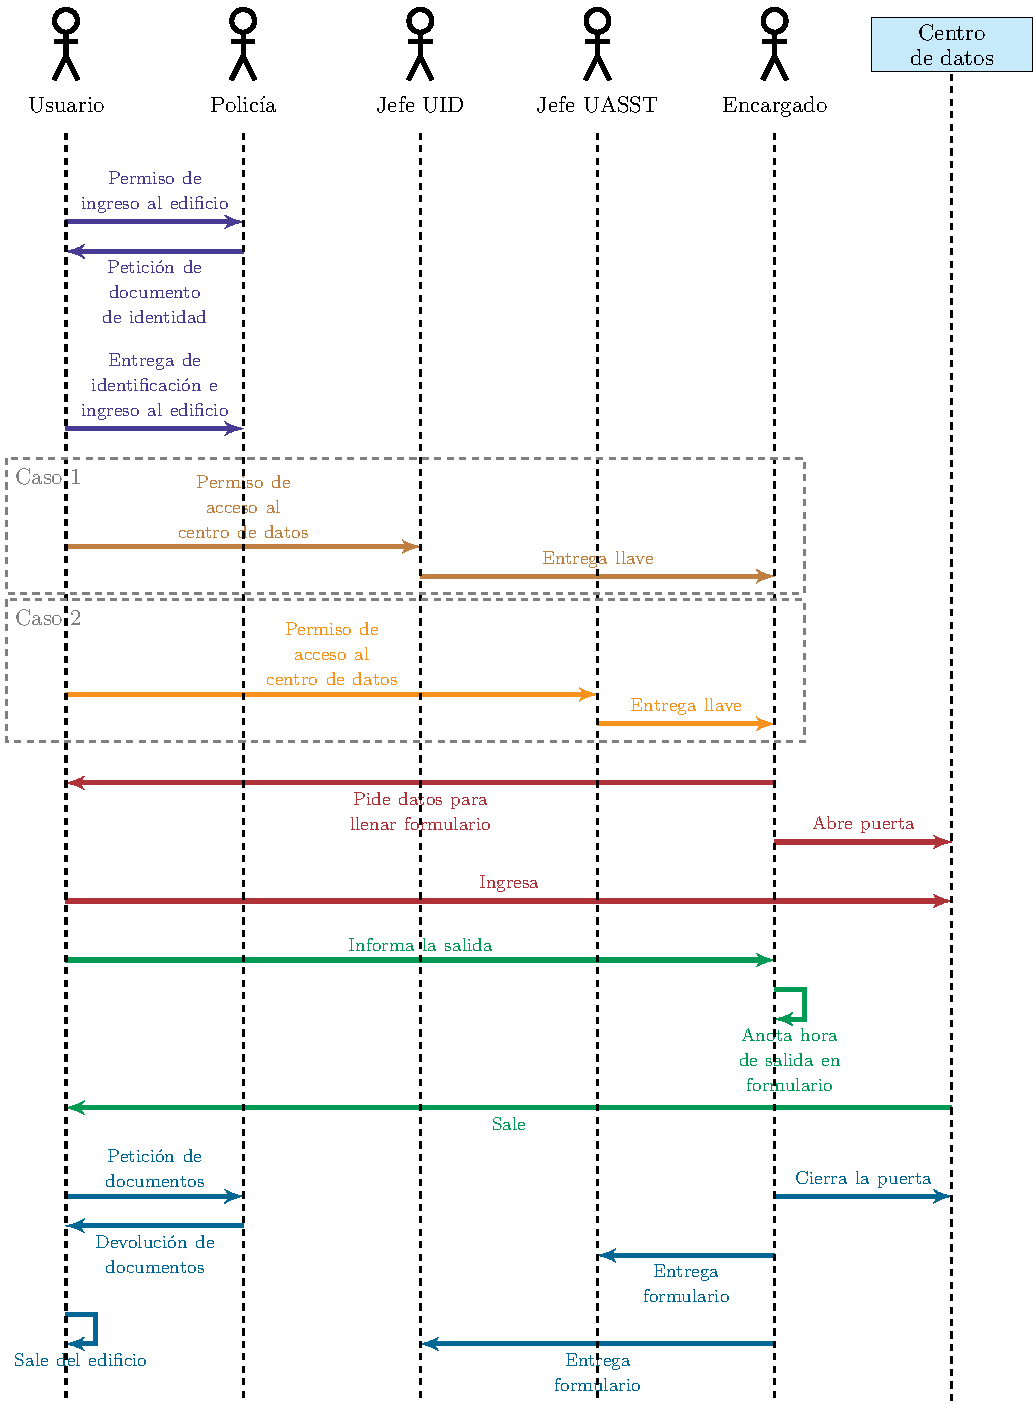
\includegraphics[width=0.95\textwidth]{flujo_ingreso_anterior.pdf}
    \caption*{\textbf{Fuente:} Elaboración propia}
    \label{fig:flujo_ingreso_anterior}
  \end{figure}

  El flujo promedio de personas que ingresa al centro de datos es de 4 personas/día, el tiempo promedio entre ingresos es de 1 vez cada 2 horas. Existen casos aislados, por ejemplo durante las auditorías donde el flujo incrementa hasta 12 personas/día y el tiempo entre ingresos promedio sube a 2 veces cada hora.

  \subsection{Especificación de requisitos a satisfacer con el desarrollo del sistema}

  Los requerimientos funcionales del sistema especificados por el Jefe de la Unidad de Innovación y Desarrollo de ADSIB se enumeran por orden de prioridad:
  \begin{enumerate}
    \item Instalar el sistema en 5 ambientes del centro de datos
    \item Utilizar un método de identificación biométrico para acceder a los ambientes
    \item La salida de los ambientes no debe contar con ningún tipo de identificación y debe ser constituida con elementos pasivos para evitar que las personas queden atrapadas en los ambientes en caso de emergencia
    \item Utilizar tecnologías de software y hardware libre en la mayor proporción posible
    \item Compatibilizar el sistema con el respaldo de energía mediante UPS disponible en el centro de datos
    \item El registro de nuevos usuarios debe realizarse en un dispositivo de hardware destinado específicamente para esa función
    \item El hardware registrador estará ubicado en la oficina de ADSIB que se encuentra tres pisos más arriba del centro de datos pero contará con conexión de red mediante un conector RJ45
    \item El sistema debe ser compatible con el servidor LDAP que almacena la lista de todo el personal de ADSIB
    \item Proveer un sistema de apertura mediante otro medio diferente al principal para la apertura de emergencia de la puerta principal
    \item El sistema de apertura alternativo deberá estar aislado del sistema central para evitar la falla simultanea de ambos sistemas
    \item Proveer un sistema de administración web que permita registrar nuevos usuarios
    \item Al momento del registro de un nuevo usuario el sistema web debe poder sincronizar los cambios producidos en el servidor LDAP
    \item El sistema web debe tener una función que permita establecer permisos a cada usuario registrado para que pueda acceder por las diferentes puertas sin una fecha final para el permiso
    \item El sistema web debe tener una función que permita establecer permisos a cada usuario registrado para que pueda acceder por una puerta de forma temporal estableciendo una fecha inicial y una fecha final
    \item En caso de tener que registrar las nuevas identidades en los sensores, este registro se debe hacer mediante el sistema web
    \item El sistema web debe mostrar la apertura de puertas en tiempo real identificando la persona que accedió y la puerta por la que accedió
    \item El sistema web debe tener la capacidad de mostrar un historial de accesos con un filtro de fechas
    \item El sistema web debe proveer otro nivel de acceso para usuarios sin permiso de administrador que permita abrir las puertas mediante botones en una página web
    \item Los usuarios sin permiso de administrador no podrán abrir puertas en el sistema web por las cuales no puedan acceder mediante el sensor biométrico
  \end{enumerate}

  \section{Perspectiva global del sistema propuesto}

  \begin{figure}[h]
    \centering
    \caption{Diagrama de bloques del sistema de control de accesos}
    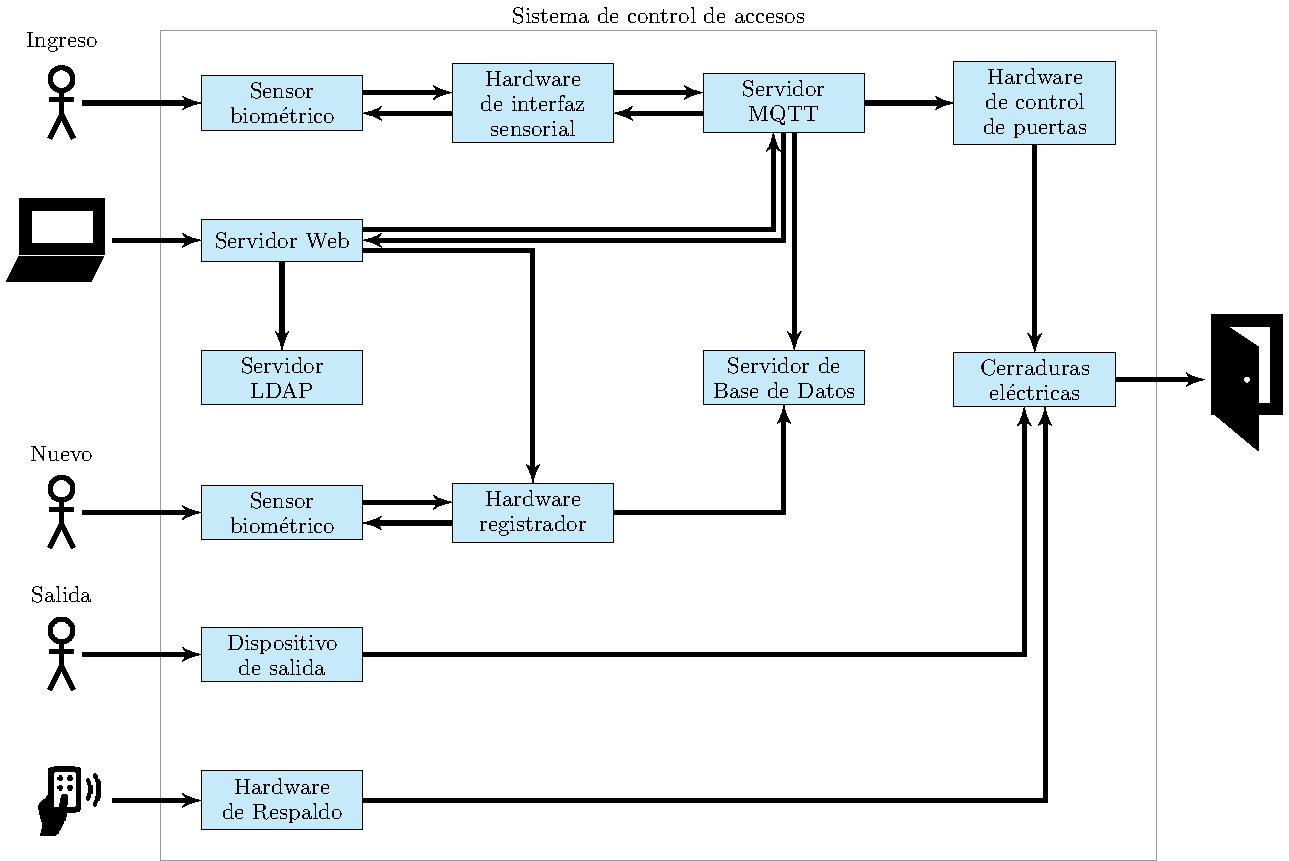
\includegraphics[width=\textwidth]{bloques_sistema_completo.pdf}
    \caption*{\textbf{Fuente:} Elaboración propia}
    \label{fig:bloques_sistema_completo}
  \end{figure}  

  \subsection{Selección del sensor biométrico}

  \subsubsection{Tasa de falso rechazo y tasa de falsa aceptación}
  
  La tasa de falso rechazo (FRR\footnote{False Rejection Rate}) es la probabilidad de que el sensor no identifique a un usuario legítimo, mientras que la tasa de falsa aceptación (FAR\footnote{False Acceptance Rate}) es la probabilidad de que el sensor identifique a un usuario ilegítimo como legítimo. Un FRR elevado provoca descontento en los usuarios ya que éstos tendrán que realizar más intentos para identificarse correctamente, pero un FAR elevado provoca graves problemas de seguridad ya que podría darse acceso a una persona no autorizada.

  Para evaluar las prestaciones de un sistema biométrico se utiliza la tasa de éxito (SR\footnote{Success Rate}), la ecuación \ref{ecu:tasa_exito_sensor} demuestra como calcular el SR.

  \vspace{-1.5em}
  \begin{equation}
    \label{ecu:tasa_exito_sensor}
    SR = 1 - (FAR + FRR)
  \end{equation}
  \vspace{-2em}

  FAR y FRR son inversamente proporcionales, para obtener un óptimo funcionamiento del sistema se debe fijar un umbral dependiendo del nivel de seguridad definido para el sistema, con este umbral se podrá identificar la tasa de error igual (EER\footnote{Equal Error Rate}), este parámetro determina la capacidad de identificación del sistema.

  \begin{figure}[H]
    \centering
    \caption{Punto de equilibrio EER}
    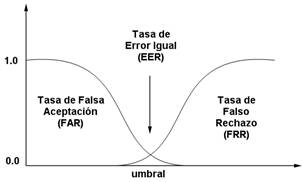
\includegraphics[width=0.6\textwidth]{ingenieria_proyecto/curvas_eer_sensor.jpg}
    \caption*{\textbf{Fuente:} Aplicación de Nuevas Tecnologías al Sistema Electoral, Sergio D. Werner\cite{web:aplicacion_sistema_electoral_biometrico}}
  \end{figure}

  El grado de seguridad deseado se define mediante el umbral de aceptación \textit{u}, un número real perteneciente al intervalo [0,1] que indica el mínimo grado de parentesco permitido para autorizar el acceso del individuo.\cite{web:aplicacion_sistema_electoral_biometrico}

  \begin{figure}[H]
    \centering
    \caption{Tasa de error vs Sensibilidad}
    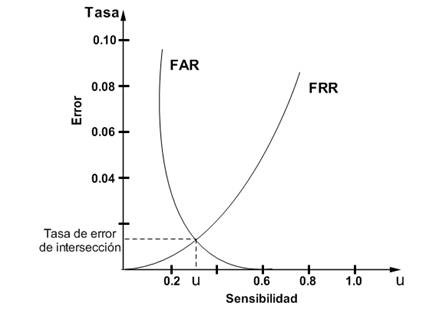
\includegraphics[width=0.7\textwidth]{ingenieria_proyecto/curvas_umbral_aceptacion_sensor.jpg}
    \caption*{\textbf{Fuente:} Aplicación de Nuevas Tecnologías al Sistema Electoral, Sergio D. Werner\cite{web:aplicacion_sistema_electoral_biometrico}}
  \end{figure}

  En base a los datos mostrados en la sección de ``Errores en sistemas biométricos'' de la monografía ``Aplicación de Nuevas Tecnologías al Sistema Electoral'' de Sergio D. Werner\cite{web:aplicacion_sistema_electoral_biometrico}, conjuntamente con la tabla mostrada en la ``Diapositiva N\degree 27'' de la presentación del ``Estudio de Dispositivos Biométricos'' de Sebastián Ramos Bustos\cite{web:soluciones_umanick} que compara las ventajas y desventajas de las tecnologías biométricas, se realizó la comparación de las características de los diferentes sensores biométricos estimando cada característica con un valor numérico del 1 al 5, donde 1 es muy bajo y 5 es muy alto, como se muestra en la Tabla \ref{tab:seleccion_sensor}.

  Del conjunto de características se calculó la estimación apreciada y con este resultado se seleccionó el método de identificación biométrica basada en la comparación de minucias de huellas dactilares.

  \begin{table}[H]
    \centering
    \caption{Características de los sensores biométricos}
    \begin{tabular}{|C{2.9cm}|C{1cm}|C{1.5cm}|C{1.8cm}|C{2.1cm}|C{1cm}|C{1.3cm}|}
  \hline
  \rowcolor[HTML]{E3FFE3}
  Característica & Ojo (iris) & Ojo (retina) & Huellas dactilares & Geometría de la mano & Voz & Rostro \\
  \hline
  Fiabilidad & 5 & 5 & 4 & 4 & 4 & 4 \\
  \hline
  Facilidad de uso & 3 & 2 & 5 & 4 & 4 & 4 \\
  \hline
  Prevención contra ataques & 5 & 5 & 4 & 4 & 3 & 3 \\
  \hline
  Aceptación & 2 & 3 & 4 & 4 & 4 & 5 \\
  \hline
  Estabilidad & 4 & 4 & 4 & 3 & 3 & 3 \\
  \hline
  Estimación apreciada & 19 & 19 & 21 & 19 & 18 & 19 \\
  \hline
\end{tabular}
    \caption*{\textbf{Fuente:} \href{http://www.monografias.com/trabajos82/biometria-y-voto-electronico/biometria-y-voto-electronico2.shtml}{Características de los rasgos biométricos, Aplicación de Nuevas Tecnologías al Sistema Electoral, Sergio D. Werner, Argentina, 9 de Marzo de 2011}}
    \label{tab:seleccion_sensor}
  \end{table}

  \begin{table}[H]
    \centering
    \caption{Comparación de sensores de huella digital}
    \begin{tabular}{|C{4cm}|C{4.5cm}|C{4.5cm}|}
  \hline
  \rowcolor[HTML]{E3FFE3}
  Característica & Sensor ZFM-20 & Sensor ARA-ME-01 \\
  \hline
  Interfaz serial & UART 9600 - 115200 bps & UART 9600 - 115200 bps \\
  \hline
  Nivel lógico & TTL & TTL \\
  \hline
  Alimentación & DC 3.6 - 6.0V & DC 5.0V \\
  \hline
  Corriente de operación & $ < $ 120mA & $ < $ 60mA \\
  \hline
  Resolución de la imagen & 256x288 pixeles & 256x288 pixeles \\
  \hline
  Memoria & 1000 huellas & 120 huellas \\
  \hline
  Precio & 50 \$us & 159.90 \$us \\
  \hline
\end{tabular}
    \caption*{\textbf{Fuente:} Elaboración propia}
    \label{tab:comparacion_sensor}
  \end{table}

  Definido el tipo de sensor a utilizar se selecciona el modelo, para esto se buscó sensores de huella dactilar disponibles en Bolivia, se encontró dos modelos comparados en la Tabla \ref{tab:comparacion_sensor} de acuerdo a los datos descritos en la tienda virtual \href{www.TecBolivia.com}{www.TecBolivia.com}.

  De la comparación de la Tabla \ref{tab:comparacion_sensor} se pudo apreciar que la memoria para huellas dactilares en el sensor ARA-ME-01 se llenaría en un plazo de tiempo más corto que la memoria del sensor ZFM-20, además que el rango de alimentación del ZFM-20 es más amplio que el ARA-ME-01, por estas razones se seleccionó el sensor de huellas digitales ZFM-20.

  El sensor ZFM-20 tiene 5 niveles de seguridad, se utilizó el nivel 3 ya que es el que tiene un umbral de aceptación más equilibrado, de acuerdo a su hoja de datos en el nivel 3 de seguridad FAR=0.001\% y FRR=0.1\% \cite{manual:fingerprint_ZFM-20}.

  Para realizar el cálculo aproximado de intentos fallidos por cada cierto número de intentos, o también el número de ataques que fallarán por cada cierto número de ataques se utiliza la Ecuación \ref{ecu:tasa_ataques_sensor}.

  \vspace{-1.5em}
  \begin{equation}
    \label{ecu:tasa_ataques_sensor}
    SR = \frac{A_r}{A_i}
  \end{equation}
  \vspace{-2em}

Para un número de 10000 intentos de ataque y los valores de FAR y FRR se reemplazan los valores en estos valores en la Ecuación \ref{ecu:intentos_fallidos_sensor} y se calcula el valor aproximado de intentos o ataques fallidos por cada 10000 intentos o ataques.

  \vspace{-1.5em}
  \begin{equation}
    \label{ecu:intentos_fallidos_sensor}
    A_r = SR \cdot A_i = [1 - (FAR + FRR)] \cdot A_i
  \end{equation}
  \vspace{-2em}

  \vspace{-1.5em}
  \begin{equation}
    A_r = [1 - (0.001 + 0.1)] \cdot 10000 = 8990
  \end{equation}
  \vspace{-2em}

  Por tanto se espera que por cada 10000 intentos, 8990 veces se reconozca correctamente la identidad de la persona que realiza el intento y 1010 veces el sensor cometerá un error de reconocimiento como falso positivo o falso negativo.

  Con base en este valor se calculó el número aproximado de veces que el sensor reconocerá un falso positivo.

  \vspace{-1.5em}
  \begin{equation}
    \label{ecu:falso_positivo_calculo}
    E_{lectura} = E_{cometidos} \cdot FAR = 1010 \cdot 0.001 = 1.01
  \end{equation}
  \vspace{-2em}

  Se puede concluir con el resultado obtenido en la Ecuación \ref{ecu:falso_positivo_calculo} que se espera que de cada 10000 intentos, el sensor cometerá el error de identificar 1 huella en una posición incorrecta de su base de datos o una huella que no se encuentre registrada como válida, valor obtenido con un nivel de seguridad 3 de acuerdo al manual del sensor ZFM-20\cite{manual:fingerprint_ZFM-20}.

  \subsection{Selección de los protocolos de comunicación}

  El punto más importante para la decisión del protocolo a utilizar fué la seguridad en el medio de transmisión, los dos medios que se pueden utilizar son el cableado e inalámbrico, se puede ver la comparación de las ventajas y desventajas entre estos dos medios en la Tabla \ref{tab:seleccion_medio_transmision}, de la cual se concluyó que el medio más conveniente para el desarrollo del proyecto es el medio cableado, porque en éste se tiene un mejor control contra ataques e infiltraciones mediante una infraestructura con una configuración óptima.

  Ahora que se seleccionó el medio físico, se procedió a la selección del medio de comunicación, para la selección se tomó como principal criterio la distancia entre el control central y las interfaces sensoriales, de acuerdo a la disposición de los ambientes del centro de datos de ADSIB se pudo realizar la medición del tramo más largo hasta donde quedaría ubicado el control central obteniendo un valor de 40m, por lo cual se compararon dos medios de comunicación RS-485 y Ethernet, de entre los cuales se seleccionó mediante el criterio de escalabilidad y se optó por Ethernet ya que el número de nodos máximo es de 65535 a comparación del RS-485 que tan solo admite 32 nodos.

  \begin{table}[H]
    \centering
    \caption{Comparativa del medio cableado vs el medio inalámbrico}
    \begin{tabular}{|C{3cm}|C{3cm}|C{3cm}|C{3cm}|}
  \hline
  \rowcolor[HTML]{FFEAD0}
  \multicolumn{2}{|c|}{Cableado} & \multicolumn{2}{|c|}{Inalámbrico} \\
  \hline
  \rowcolor[HTML]{E3FFE3}
  Ventaja & Desventaja & Ventaja & Desventaja \\
  \hline
  No se pueden interceptar señales sin conexión física a la misma red & El cable puede ser destruido & No necesita infraestructura para cada punto cliente & Rango de señal limitada \\
  \hline
  Velocidades de transmisión muy elevadas &  & Se puede expandir el área de servicio con repetidores de señal & La señal puede ser interceptada fácilmente \\
  \hline
  Los cables necesarios no son costosos &  &  & Las señales son afectadas por interferencia de otras señales \\
  \hline
  No precisa configuración en la conexión &  &  & La velocidad de transmisión es más baja que el medio cableado \\
  \hline
\end{tabular}
    \caption*{\textbf{Fuente:} Elaboración propia}
    \label{tab:seleccion_medio_transmision}
  \end{table}

  Recientemente se produjo un cambio de paradigma en el campo de recolección de datos de sensores desde el desarrollo de IoT, en este enfoque sobresalen algunos protocolos que son comparados en la Tabla \ref{tab:seleccion_protocolo_iot}.

  \begin{table}[H]
    \centering
    \caption{Comparación entre protocolos IoT}
    \begin{tabular}{|C{3cm}|C{11cm}|}
  \hline
  \rowcolor[HTML]{E3FFE3}
  Protocolo & Características \\
  \hline
  \multirow{5}{*}{MQTT} & Tamaño de paquete muy pequeño \\
  & Comunicación doble vía \\
  & Bajo consumo de energía \\
  & NAT transversal es direccionado entre redes \\
  & Hasta 10000 clientes \\
  \hline
  \multirow{5}{*}{CoAP} & Orientado a la arquitectura de servicios web \\
  & Comunicación doble vía \\
  & Fácil configuración de dispositivos para acceso a Internet \\
  & El direccionamiento NAT transversal es muy problemático \\
  & Hasta 10000 clientes \\
  \hline
  \multirow{5}{*}{API REST} & Comunicación de vía única \\
  & El direccionamiento NAT transversal es muy sencillo \\
  & Adaptado para buen funcionamiento en redes inalámbricas \\
  & Tamaño de paquete muy grande en comparación a los demás \\
  & No tiene límite de clientes \\
  \hline
  \multirow{5}{*}{XMPP} & Adaptado para soportar mucho tráfico en la red \\
  & Tamaño de paquete muy grande en comparación a los demás \\
  & Áltamente seguro en la transmisión de datos \\
  & Precisa de software o hardware para cifrado de datos \\
  & Hasta 100000 clientes \\
  \hline
\end{tabular}
    \caption*{\textbf{Fuente:} Elaboración propia}
    \label{tab:seleccion_protocolo_iot}
  \end{table}
  
  La característica buscada es la mejor compatibilidad del protocolo con una red local ya que los dispositivos no gozan de conexión a Internet, otra característica importante fué el direccionamiento NAT, ya que se propuso el desarrollo de este sistema sobre una infraestructura de red previamente instalada de la cual no se conocía la topología. Con estas características se seleccionó MQTT como protocolo de comunicación para los dispositivos del sistema.

  El protocolo MQTT mejor conocido como Mosquitto, es un protocolo desarrollado por IBM para la comunicación Máquina-Máquina (M2M). Desde 2013 es catalogado como el estándar ISO/IEC PRF 20922, es una alternativa más ligera que AMQP, XMPP o WAMP. Se ubica dentro de la capa de aplicación del modelo OSI en base al protocolo TCP/IP.

  Este protocolo se basa en la topología de suscripción a tópicos y publicación de mensajes. Se puede implementar sobre una capa segura SSL, brindando la posibilidad de cifrado de los datos al momento de enviar o recibir mensajes, además implementa permisos de acceso al momento de la conexión mediante la combinación usuario/contraseña, y se pueden definir permisos para publicación o suscripción en diferentes tópicos para cada cliente.

  \begin{table}[H]
    \centering
    \caption{Comparación de envío de mensajes entre HTTPS y MQTT}
    \caption*{Enviando 1024 mensajes con carga útil de 1 byte}
    \begin{tabular}{|r|c|c|c|c|}
  \cline{2-5}
  \hhline{~--|--|}
  \rowcolor[HTML]{FFEAD0}
  \multicolumn{1}{c|}{\cellcolor[HTML]{FFFFFF}} & \multicolumn{2}{c|}{3g} & \multicolumn{2}{c|}{Wi-Fi} \\
  \hhline{~|-|-|-|-|}
  \rowcolor[HTML]{E3FFE3}
  \multicolumn{1}{c|}{\cellcolor[HTML]{FFFFFF}} & \multicolumn{1}{c|}{HTTPS} & MQTT & HTTPS & MQTT \\
  \hline
  \cellcolor[HTML]{E4FFFE}\% Batería / Hora & 18,79\% & \textbf{17,80\%} & 5,44\% & \textbf{3,66\%} \\
  \hline
  \cellcolor[HTML]{E4FFFE}Mensajes / Hora & 1926 & \textbf{21685} & 5229 & \textbf{23184} \\
  \hline
  \cellcolor[HTML]{E4FFFE}\% Batería / Mensaje & 0,00975 & \textbf{0,00082} & 0,00104 & \textbf{0,00016} \\
  \hline
\end{tabular}
    \caption*{\textbf{Fuente:} \href{http://stephendnicholas.com/posts/power-profiling-mqtt-vs-https}{Power Profiling: HTTPS Long Polling vs. MQTT with SSL, on Android, Blog de Stephen Nicholas, 31 de Mayo de 2012}}
    \label{tab:comparacion_http_mqtt_envio}
  \end{table}

El dispositivo central llamado broker, puede gestionar y transmitir los mensajes de hasta 10.000 clientes. Por otro lado la ventaja más grande en comparación con el protocolo HTTP es que MQTT no tiene un tamaño de paquete fijo, ya que el mismo se adapta de acuerdo al tipo de conexión y al tipo de mensaje enviado, solo necesita 69 bytes para un mensaje vacío mientras que HTTP necesita 302 bytes para un mensaje vacío. La cabecera de MQTT ocupa tan solo 2 bytes al contrario de HTTP cuya longitud mínima de cabecera es de 18 bytes. La carga útil de MQTT es de 0B a 256MB.

  \begin{table}[H]
    \centering
    \caption{Comparación de recepción de mensajes entre HTTPS y MQTT}
    \caption*{Recibiendo 1024 mensajes con carga útil de 1 byte}
    \begin{tabular}{|r|c|c|c|c|}
  \hhline{~--|--|}
  \rowcolor[HTML]{FFEAD0}
  \multicolumn{1}{c|}{\cellcolor[HTML]{FFFFFF}} & \multicolumn{2}{c|}{3g} & \multicolumn{2}{c|}{Wi-Fi} \\
  \hhline{~|-|-|-|-|}
  \rowcolor[HTML]{E3FFE3}
  \multicolumn{1}{c|}{\cellcolor[HTML]{FFFFFF}} & \multicolumn{1}{c|}{HTTPS} & MQTT & HTTPS & MQTT \\
  \hline
  \cellcolor[HTML]{E4FFFE}\% Batería / Hora & 18,43\% & \textbf{16,13\%} & \textbf{3,45\%} & 4,23\% \\
  \hline
  \cellcolor[HTML]{E4FFFE}Mensajes / Hora & 1708 & \textbf{160278} & 3628 & \textbf{263314} \\
  \hline
  \cellcolor[HTML]{E4FFFE}\% Batería / Mensaje & 0,01709 & \textbf{0,0001} & 0,00095 & \textbf{0,00002} \\
  \hline
  \cellcolor[HTML]{E4FFFE}Mensajes Recibidos & 240 / 1024 & \textbf{1024 / 1024} & 524 / 1024 & \textbf{1024 / 1024} \\
  \hline
\end{tabular}
    \caption*{\textbf{Fuente:} \href{http://stephendnicholas.com/posts/power-profiling-mqtt-vs-https}{Power Profiling: HTTPS Long Polling vs. MQTT with SSL, on Android, Blog de Stephen Nicholas, 31 de Mayo de 2012}}
    \label{tab:comparacion_http_mqtt_recepcion}
  \end{table}

  \begin{table}[H]
    \centering
    \caption{Comparación de consumo de batería con señales de Keep Alive}
    \begin{tabular}{|c|c|c|c|c|}
  \hhline{~|----|}
  \multicolumn{1}{l|}{} & \multicolumn{4}{c|}{\cellcolor[HTML]{ECF4FF}\% Bateria / Hora} \\
  \hhline{~--|--|}
  \rowcolor[HTML]{FFEAD0}
  \multicolumn{1}{c|}{\cellcolor[HTML]{FFFFFF}} & \multicolumn{2}{c|}{3g} & \multicolumn{2}{c|}{Wi-Fi} \\
  \hline
  \rowcolor[HTML]{E3FFE3}
  Keep Alive (segundos) & HTTPS & MQTT & HTTPS & MQTT \\
  \hline
  60 & 1.11553 & \textbf{0.72465} & 0.15839 & \textbf{0.01055} \\
  \hline
  120 & 0.48697 & \textbf{0.32041} & 0.08774 & \textbf{0.00478} \\
  \hline
  240 & 0.33277 & \textbf{0.16027} & 0.02897 & \textbf{0.00230} \\
  \hline
  480 & 0.08263 & \textbf{0.07991} & 0.00824 & \textbf{0.00112} \\
  \hline
\end{tabular}
    \caption*{\textbf{Fuente:} \href{http://stephendnicholas.com/posts/power-profiling-mqtt-vs-https}{Power Profiling: HTTPS Long Polling vs. MQTT with SSL, on Android, Blog de Stephen Nicholas, 31 de Mayo de 2012}}
    \label{tab:comparacion_http_mqtt_keep_alive}
  \end{table}

  Las datos observados en las Tablas \ref{tab:comparacion_http_mqtt_envio}, \ref{tab:comparacion_http_mqtt_recepcion} y \ref{tab:comparacion_http_mqtt_keep_alive} fueron generados con un teléfono inteligente HTC Desire sobre el sistema operativo Android 2.2.2 - Compilación 2.33.161.6 CL345089.

  La medida ``\% Batería / Hora'' \ tiene referencia a una carga completa de la batería de Li-Ion de capacidad de 3.7V y 1400mAh.

  La aplicación que se utilizó para obtener los datos es \href{http://ziyang.eecs.umich.edu/projects/powertutor/}{PowerTutor}, que produce un margen de error entre 0.8\% y 2.5\%.

  Por lo tanto el protocolo MQTT es el más conveniente para el desarrollo de este sistema.

  En cuanto a los protocolos para el sistema de administración web se seleccionó REST en lugar de SOAP\footnote{Simple Object Access Protocol} ya que los datos se intercambiarán mediante mensajes en formato JSON\footnote{JavaScript Object Notation} y no XML\footnote{eXtensible Markup Language} y para el servidor web se utilizó HTTP/2\footnote{HyperText Transfer Protocol} que entre sus ventajas principales sobre HTTP1.1 tiene el cifrado obligatorio de datos y el formato binario para el intercambio de datos que permite mostrar mensajes en tiempo real con un retardo menor al intercambio de mensajes en ASCII de HTTP1.1.

  \subsection{Selección del dispositivo de procesamiento de datos para el hardware de control y la interfaz sensorial} \label{seleccion_atmega328}

  Se propuso un sistema escalable mediante el uso de un mismo hardware para el control de puertas y la interfaz sensorial que se ubicó en cada puerta, para este dispositivo se seleccionó entre un microprocesador y un microcontrolador, las operaciones a realizar por el hardware son el control de salidas digitales para la apertura de puertas y la transmisión serial con el sensor de huellas dactilares, las placas de desarrollo que se encontraron disponibles en el mercado para este fin fueron Arduino, Raspberry y CubieBoard.
  
  \begin{wrapfigure}[10]{r}{0.5\textwidth}
    \centering
    \caption{Arduino UNO SMD R3}
    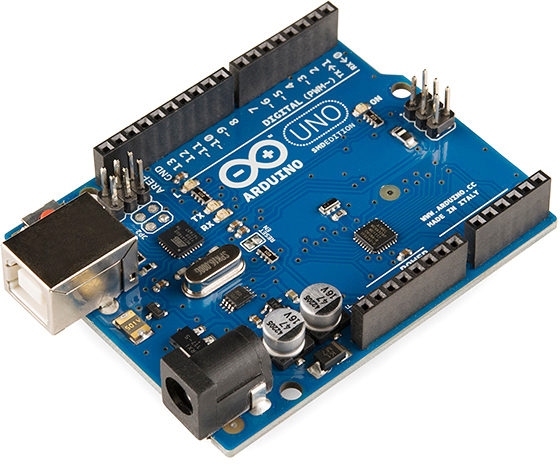
\includegraphics[width=0.4\textwidth]{marco_teorico/arduino_uno.jpg}
    \caption*{\textbf{Fuente:} \href{https://en.wikipedia.org/wiki/Arduino}{Wikipedia}}
  \end{wrapfigure}

  De entre estas tres opciones se seleccionó Arduino porque éste cuenta con lo necesario para ejecutar las operaciones definidas para el sistema y tanto el diseño, la programación e instalación serían más fáciles, además Arduino garantizaría la estabilidad del sistema ya que el programa se encuentra encapsulado en la memoria Flash que no es accesible, a diferencia de la tarjeta SD que necesitan las tarjetas de desarrollo basadas en microprocesadores.

  A continuación se debía seleccionar un modelo de Arduino, la tienda virtual de referencia \href{www.TecBolivia.com}{www.TecBolivia.com} disponía de microcontroladores: ATmega328P, ATmega32U2, ATmega32U4 y ATtiny85. Los dos microcontroladores que tienen compatibilidad con los módulos de red son ATmega328P y ATtiny85, la característica para la selección fué la capacidad de memoria Flash ya que el programa ocupa 23.336KB y la memoria del ATtiny85 tan solo cuenta con 8KB, por lo cual se seleccionó el microcontrolador ATmega328P, con la ventaja adicional de que en el desarrolló se pudo utilizar la placa Arduino UNO.

  \subsubsection{Selección del dispositivo controlador Ethernet para el hardware de control y la interfaz sensorial}

  Arduino es compatible con dos dispositivos controladores de Ethernet, éstos son el circuito integrado W5100 y el integrado ENC28J60, en el mercado solo se pudo encontrar el circuito integrado ENC28J60, por lo tanto la placa de desarrollo seleccionada fué Ethercard.

  \begin{figure}[H]
    \centering
    \caption{Ethercard}
    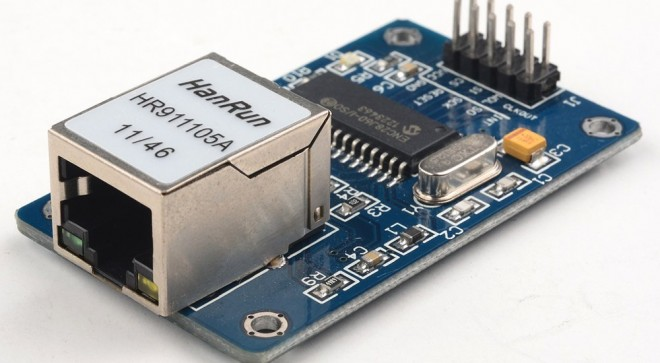
\includegraphics[width=0.3\textwidth]{marco_teorico/ethercard.jpg}
    \caption*{\textbf{Fuente:} \href{http://www.michaelbrich.com/using-the-enc28j60-ethernet-module-with-an-arduino-mega-2560/}{Usando el Módulo Ethernet ENC28J60, Blog de Michael Brich, 24 de Marzo de 2015}}
  \end{figure}

    Ethercard es una tarjeta de desarrollo para el circuito integrado ENC28J60, compatible con arduino, mediante el protocolo SPI (Serial Peripheral Interface) con una velocidad de hasta 10 Mb/s. Este chip es compatible con el estándar IEEE 802.3i y contiene toda la lógica anti-colisión y de rechazo de paquetes erróneos, listo para una conexión TCP/IP. También tiene opción para instalar 2 leds, uno para indicar el enlace y otro para indicar la transmisión de datos. Este circuito integrado necesita de un reloj externo que oscile a 25 MHz y una fuente de alimentación de 3.3V, pero las entradas de control trabajan en los niveles TTL de 5V. Se debe asignar una dirección MAC mediante software para identificar este hardware en la red.

  \subsubsection{Selección de la frecuencia de reloj para el microcontrolador ATmega328P}

  El principal criterio para la selección del reloj fué la conexión con el sensor de huellas. En base al esquema de Arduino UNO R3 [Anexo \ref{anx:esquematico_arduino_uno}], de donde se conservó sólo la etapa de comunicación serial para la conexión con el sensor de huellas y cuatro pines digitales para las salidas hacia los relés para la apertura de puertas, se tuvo dos opciones, utilizar el reloj interno o uno externo.

  Por defecto la placa Arduino UNO R3 trabaja a 16Mhz, que es una frecuencia totalmente compatible con la tasa de bits a la que trabaja el sensor de huellas, que por defecto es de 57600bps. Aunque también se podía utilizar el reloj interno de 8Mhz que incorpora el ATmega328P como se indica en su hoja de datos \cite{datasheet:atmega328}, se eligió utilizar un reloj externo de 16MHz de acuerdo a las reglas de diseño especificadas en el artículo \textit{Determining Clock Accuracy Requirements for UART Communications} \cite{reporte:determinando_precision_reloj_comunicacion_uart} y las ecuaciones obtenidas del Manual del ATmega328P \cite{datasheet:atmega328}, el primer paso es identificar un valor para el registro UxBRG (BaudRate Generator), mayormente conocido como variable BSEL para el cual se aplica la siguiente ecuación:

  \vspace{-1.5em}
  \begin{equation}
    \label{calculo_bsel_uart}
    BSEL = \frac{f_{PER}}{2^{BSCALE} \cdot 16f_{BAUD}} - 1
  \end{equation}
  \vspace{-2em}

  Donde: $ f_{PER} $ es la frecuencia del periférico, BSCALE toma el valor de 0 para conexión UART asíncrona en modo normal y $ f_{BAUD} $, es la velocidad de conexión a la que se desea llegar.

  Insertando los valores numéricos se calcula BSEL:

  \vspace{-1.5em}
  \begin{equation}
    \label{calculo_numerico_bsel_uart}
    BSEL = \frac{16000000}{2^{0} \cdot 16 \cdot 57600} - 1 = 16.361 \simeq 16
  \end{equation}
  \vspace{-2em}

  El valor de BSEL debe ser un número entero ya que es el valor que tomará un registro de control en el ATMEGA328P. Despejando de la ecuación Nº \ref{calculo_bsel_uart}

  \vspace{-1.5em}
  \begin{equation}
    \label{calculo_numerico_uart}
    f_{BAUD}* = \frac{f_{PER}}{2^{BSCALE} \cdot 16 \cdot (BSEL + 1)}
  \end{equation}
  \vspace{-2em}

  Insertando los valores numéricos se calcula $ f_{BAUD} $:

  \vspace{-1.5em}
  \begin{equation}
    \label{calculo_numerico_f_baud}
    f_{BAUD}* = \frac{16000000}{2^{0} \cdot 16 \cdot (16 + 1)} = 58824.53
  \end{equation}
  \vspace{-2em}

  Ahora se calcula el error de tasa de bits, que según el estándar TIA RS-232C\footnote{Telecommunications Industry Association - Recommended Standard 232} debe ser menor a 3\%:

  \vspace{-1.5em}
  \begin{equation}
    \label{calculo_error_uart}
    err_{f} = \frac{f_{BAUD}* - f_{BAUD}}{f_{BAUD}} * 100\%
  \end{equation}
  \vspace{-2em}

  Insertando los valores numéricos se calcula $ err_{f} $:

  \vspace{-1.5em}
  \begin{equation}
    \label{calculo_numerico_error_uart}
    err_{f} = \frac{58824.53 - 57600}{57600} * 100\% = 2.12\%
  \end{equation}
  \vspace{-2em}

  Si se realizan los cálculos en base al reloj interno de 8MHz se obtiene un error de -3.54\% que se encuentra por encima del valor estándar, es por ello que se diseñó el circuito con un reloj externo de 16MHz para el microcontrolador ATmega328P.

  \begin{figure}[h]
    \centering
    \caption{Captura de forma de onda de transmisión serial a 57600Hz}
    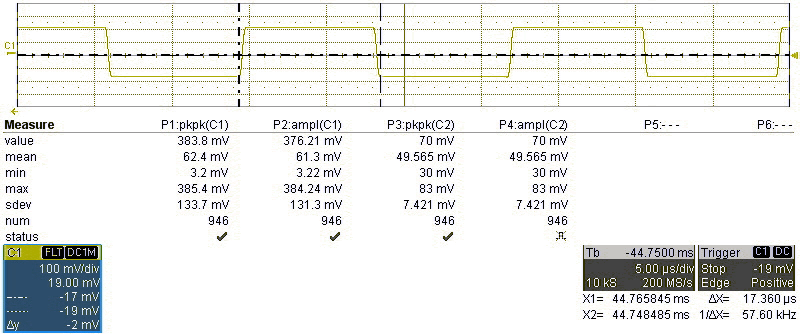
\includegraphics[width=0.95\textwidth]{ingenieria_proyecto/osciloscopio_baudrate_ideal.png}
    \caption*{\textbf{Fuente:} Elaboración propia}
    \label{fig:osciloscopio_baudrate_ideal}
  \end{figure}

  \begin{figure}[h]
    \centering
    \caption{Captura de forma de onda de transmisión serial a 58824Hz}
    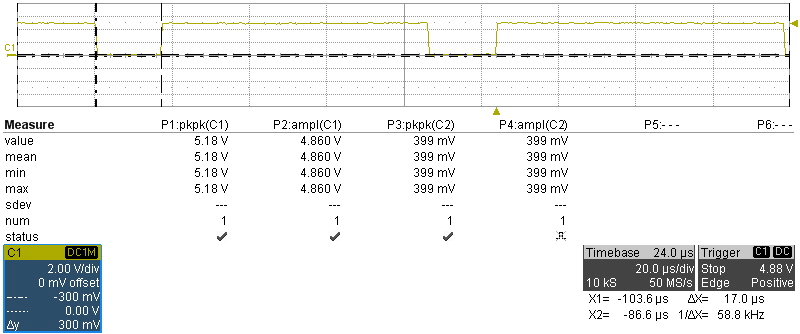
\includegraphics[width=0.95\textwidth]{ingenieria_proyecto/osciloscopio_baudrate_real.png}
    \caption*{\textbf{Fuente:} Elaboración propia}
    \label{fig:osciloscopio_baudrate_real}
  \end{figure}

  En las tablas \ref{tabla_error_tasa_clock_uart_8MHz} y \ref{tabla_error_tasa_clock_uart_16MHz} se muestra un cálculo completo en base a las Ecuaciones \ref{calculo_bsel_uart}, \ref{calculo_numerico_uart}, \ref{calculo_error_uart} para los dos valores de reloj interno y externo respectivamente, de acuerdo a los valores de tasa de bits a los que se comunica el sensor de huellas dactilares, tomando en cuenta que la librería de comunicación serial de Arduino establece el registro U2Xn o BSCALE en 0.

  \begin{table}[H]
    \caption{Error de tasa de bits a 8MHz}
    \label{tabla_error_tasa_clock_uart_8MHz}
    \centering
    \begin{tabular}{|c|c|c|c|c|}
  \hline
  \rowcolor[HTML]{FFEAD0} \multicolumn{5}{|c|}{$ f_{PER} $ = 8.0000 MHz} \\
  \hline
  \rowcolor[HTML]{E3FFE3} $ f_{BAUD} $(bps) & BSEL & BSEL(hex) & $ f_{BAUD} $*(bps) & Error \\
  \hline
  9.6K & 51 & 0x33 & 9.61K & 0.2\% \\
  \hline
  19.2K & 25 & 0x19 & 19.23K & 0.2\% \\
  \hline
  28.8K & 16 & 0x10 & 29.412K & 2.1\% \\
  \hline
  38.4K & 12 & 0x0C & 38.462K & 0.2\% \\
  \hline
  48K & 9 & 0x09 & 50K & 4.2\% \\
  \hline
  57.6K & 8 & 0x08 & 55.556K & -3.5\% \\
  \hline
  62.7K & 7 & 0x07 & 62.5K & -0.3\% \\
  \hline
  76.8K & 6 & 0x06 & 71.429K & -7.0\% \\
  \hline
  86.4K & 5 & 0x05 & 83.333K & -3.5\% \\
  \hline
  96K & 4 & 0x04 & 100K & 4.2\% \\
  \hline
  105.6K & 4 & 0x04 & 100K & -5.3\% \\
  \hline
  115.2K & 3 & 0x03 & 125K & 8.5\% \\
  \hline
\end{tabular}
    \caption*{\textbf{Fuente:} Elaboración propia}
  \end{table}

  Como se puede observar en la tabla \ref{tabla_error_tasa_clock_uart_8MHz} el error a una tasa de bits por arriba de los 62.7Kbps se eleva hasta los 8.5\%, valor que se desvía demasiado del estándar. Con una frecuencia de reloj de 16Mhz se obtienen mejores resultados en cuanto a la variación de tasa de bits.

  \begin{table}[H]
    \caption{Error de tasa de bits a 16MHz}
    \label{tabla_error_tasa_clock_uart_16MHz}
    \centering
    \begin{tabular}{|c|c|c|c|c|}
  \hline
  \rowcolor[HTML]{FFEAD0} \multicolumn{5}{|c|}{$ f_{PER} $ = 16.0000 MHz} \\
  \hline
  \rowcolor[HTML]{E3FFE3} $ f_{BAUD} $(bps) & BSEL & BSEL(hex) & $ f_{BAUD} $*(bps) & Error \\
  \hline
  9.6K & 103 & 0x67 & 9.61K & 0.2\% \\
  \hline
  19.2K & 51 & 0x33 & 19.23K & 0.2\% \\
  \hline
  28.8K & 34 & 0x22 & 28.571K & -0.8\% \\
  \hline
  38.4K & 25 & 0x19 & 38.462K & 0.2\% \\
  \hline
  48K & 20 & 0x14 & 47.619K & -0.8\% \\
  \hline
  57.6K & 16 & 0x10 & 58.824K & 2.1\% \\
  \hline
  62.7K & 15 & 0x0F & 62.5K & -0.3\% \\
  \hline
  76.8K & 12 & 0x0C & 76.923K & 0.2\% \\
  \hline
  86.4K & 11 & 0x0B & 83.333K & -3.5\% \\
  \hline
  96K & 9 & 0x09 & 100K & 4.2\% \\
  \hline
  105.6K & 8 & 0x08 & 111.111K & 5.2\% \\
  \hline
  115.2K & 8 & 0x08 & 111.111K & -3.5\% \\
  \hline
\end{tabular}
    \caption*{\textbf{Fuente:} Elaboración propia}
  \end{table}

  En la Figura \ref{fig:osciloscopio_baudrate_ideal} se muestra la captura de un osciloscopio que capturó la forma de onda otorgada por un generador de funciones a 57.6KHz, donde se observa que el tiempo de cada bit es de 17.36$ \mu $s. De la misma forma en la Figura \ref{fig:osciloscopio_baudrate_real} se muestra la captura de un osciloscopio que capturó la forma de onda durante la transmisión serial entre el Arduino UNO y el sensor serial a 57600bps, donde se observa que el tiempo de cada bit es de 17.0$ \mu $s, y además se observa que la frecuencia es de 58.8Khz.

  Por lo tanto se demuestra que la transmisión serial asíncrona que existe entre el Arduino UNO y el sensor biométrico ZFM-20 a 57600bps idealmente, en la práctica es de 58824bps produciendo un error del 2.1\% como se demostró en la Ecuación \ref{calculo_numerico_error_uart}. Por lo tanto la frecuencia de reloj seleccionada para el ATmega328P fué de 16MHz.

  \subsection{Selección del núcleo del dispositivo registrador de nuevas huellas}

  Para la selección del núcleo del registrador de nuevas huellas se tomó en cuenta a los dispositivos con conexión serial, Ethernet y que además tengan acceso a realizar consultas y operaciones en la base de datos, para ello se buscaron opciones en la tienda virtual \href{www.TecBolivia.com}{www.TecBolivia.com} y entre las opciones de dispositivos con estas características se encontraron dos placas de desarrollo Cubieboard y Raspberry Pi.

  En cuanto a Raspberry Pi, se descartó el modelo A ya que no tiene soporte para conexión Ethernet, se descartó también el modelo 2 en favor del modelo 3 ya que ambos tienen el mismo costo pero el modelo 2 tiene prestaciones menores al modelo 3. 

  Por lo tanto la comparación se realizó entre las placas de desarrollo Cubieboard ARM Cortex-A8 Mini PC, Cubieboard2 ARM Cortex-A7 Dual Core Mini PC y Raspberry Pi Modelo B Version 3 cuya comparación se muestra en la Tabla \ref{tab:comparacion_cubieboard_raspberry}.

  Gracias a esta comparación se seleccionó la placa de desarrollo Raspberry Pi Modelo B Versión 3 Mini PC porque tiene 2 núcleos más que la placa Cubieboard2 y 3 más que la placa Cubieboard, además la arquitectura es de 64 bits en comparación con los 32 bits de las placas Cubieboard y tiene incorporado un circuito para conexión Wi-Fi.

  Por otro lado las placas Cubieboard tienen bondades como una entrada de señal de frecuencia modulada o el conversor analógico-digital que incrementan su precio y en este caso no tendrán ninguna funcionalidad.

  \begin{table}[H]
    \caption{Comparación Raspberry vs Cubieboard}
    \label{tab:comparacion_cubieboard_raspberry}
    \centering
    \begin{tabular}{|C{3cm}|C{3.5cm}|C{3.5cm}|C{3.5cm}|}
  \hline
  \rowcolor[HTML]{E3FFE3}
  Característica & Cubieboard ARM Cortex-A8 & Cubieboard2 ARM Cortex-A7 & Raspberry Pi Modelo B Version 3\\
  \hline
  Procesador & SoC A10 ARM® Cortex™-A8 & SoC A20 ARM® Cortex™-A7 Dual-Core & SoC ARM® Cortex™-A53 Quad Core \\
  \hline
  Frecuencia de Clock & 1.0Ghz & 1.2GHz & 1.2GHz \\
  \hline
  Arquitectura & 32bits & 32bits & 64bits \\
  \hline
  Memoria RAM & 1GB DDR3 & 1GB DDR3 & 1GB DDR3 \\
  \hline
  Memoria de programa & 4GB Flash NAND & 4GB Flash NAND & - \\
  \hline
  Salida de video & HDMI 1080p & HDMI 1080p & HDMI 1080p, RAW LCD \\
  \hline
  Almacenamiento externo & Micro SD, SATA (+5v power) & Micro SD, SATA (+5v power) & Micro SD \\
  \hline
  Ethernet & 10/100M & 10/100M & 10/100M \\
  \hline
  WiFi & - & - & BCM43143 \\
  \hline
  Alimentacion & 5V @ 2A & 5V @ 2A & 5V @ 2.4 A via microUSB \\
  \hline
  GPIO & 96 pines & 96 pines & 40 pines \\
  \hline
  Sistemas operativos & Ubuntu, Android & Ubuntu 12.04, Android 4.2.2 & Raspbian, Windows 10 IoT Core, Pidora, Arch Linux \\
  \hline
  Precio & 98\$us & 118\$us & 70.30\$us \\
  \hline
\end{tabular}

    \caption*{\textbf{Fuente:} Elaboración propia}
  \end{table}

  \subsection{Selección del método de respaldo}

  Para la selección del método de respaldo se descartó el método de panel numérico por el estrecho espacio que existe en los ambientes del centro de datos para colocar un dispositivo al ingreso de cada puerta, por tanto se selecciono un método que también se basa en contraseñas numéricas pero que no precisa de un espacio visible en la instalación, el método seleccionado fué un circuito bluetooth.

  \subsubsection{Selección del módulo bluetooth}

  Se seleccionó el módulo bluetooth HC-06 porque solo se necesita que el módulo trabaje como esclavo y no como maestro, por eso se descartó el módulo bluetooth HC-05.

  \subsubsection{Selección del dispositivo de procesamiento de datos}

  Como ya se mencionó, para la selección de este dispositivo se tomó más en cuenta el espacio que ocuparía la placa desarrollada, por tanto se seleccionó el otro microcontrolador disponible en el mercado, el ATtiny85 que tiene las características suficientes para manejar dos relés para controlar la apertura de las puertas y conectarse con el módulo bluetooth HC-06.

  Para la conexión con este dispositivo se desarrollo una aplicación en Android con la cual se envían las contraseñas almacenadas en la memoria del dispositivo con las cuales se abren las puertas controladas por este dispositivo en caso de que el sistema de control de accesos o el sensor de huellas presenten fallas.

  \subsection{Selección de la cerradura eléctrica}

  Para seleccionar la cerradura eléctrica se realizaron pruebas con 2 tipos de cerraduras, las de contacto magnético y las de tornillo tipo BOLT. Se seleccionó la cerradura de tornillo ya que la cerradura de contacto magnético cedía ante fuerzas aplicadas para forzar la apertura de la cerradura.

  \subsection{Selección de la base de datos}

  Ya que los datos tienen relación entre sí, se definió utilizar una base de datos SQL.
  
  Para la selección del gestor de bases de datos se tomó como principal criterio la seguridad al momento de la conexión con la base de datos y las licencias de código abierto, por lo cual se descartó SQLite ya que no cuenta con un método de seguridad para filtrar IPs o hosts que intentan conectarse con la base de datos, por tanto las opciones que quedaron fueron MySQL y PostgreSQL. Ambas cuentan con las características que se buscan pero PostgreSQL cuenta con una adicional, la de reacción ante eventos o cambios en los datos, por lo tanto PostgreSQL se enfoca en la adquisición y monitoreo de datos en tiempo real, esta es la característica necesaria para realizar el monitoreo en el sistema web desarrollado, por lo tanto la base de datos que se utilizó en el proyecto fué PostgreSQL.

  \subsection{Diagrama de red del sistema de control de accesos}

  El diagrama de la Figura \ref{fig:topologia_red_sistema_completo} muestra que la instalación se realizó en base a una topología desconocida entre el cliente y el sistema, pero para evitar ataques de spoofing o de suplantación de identidad se tiene un router que contiene reglas específicas para que solo las direcciones MAC de los dispositivos de interfaz sensorial, el controlador de puertas y el registrador de nuevas huellas puedan acceder a los servidores MQTT, LDAP y de bases de datos. Por otra parte los clientes conectados a la red pueden acceder al servidor web sin ninguna restricción, esto no conlleva ningún riesgo ya que se cuenta con métodos de seguridad mediante login con credenciales de usuario y contraseña a los que el servidor devuelve un token en formato JSON para mantener la sesión activa por un tiempo determinado.

  El Switch POE instalado es de 24 puertos previendo la escalabilidad del sistema a futuro, este Switch POE es compatible con el estándar 802.3af.

  \begin{figure}[H]
    \centering
    \caption{Diagrama de red del sistema}
    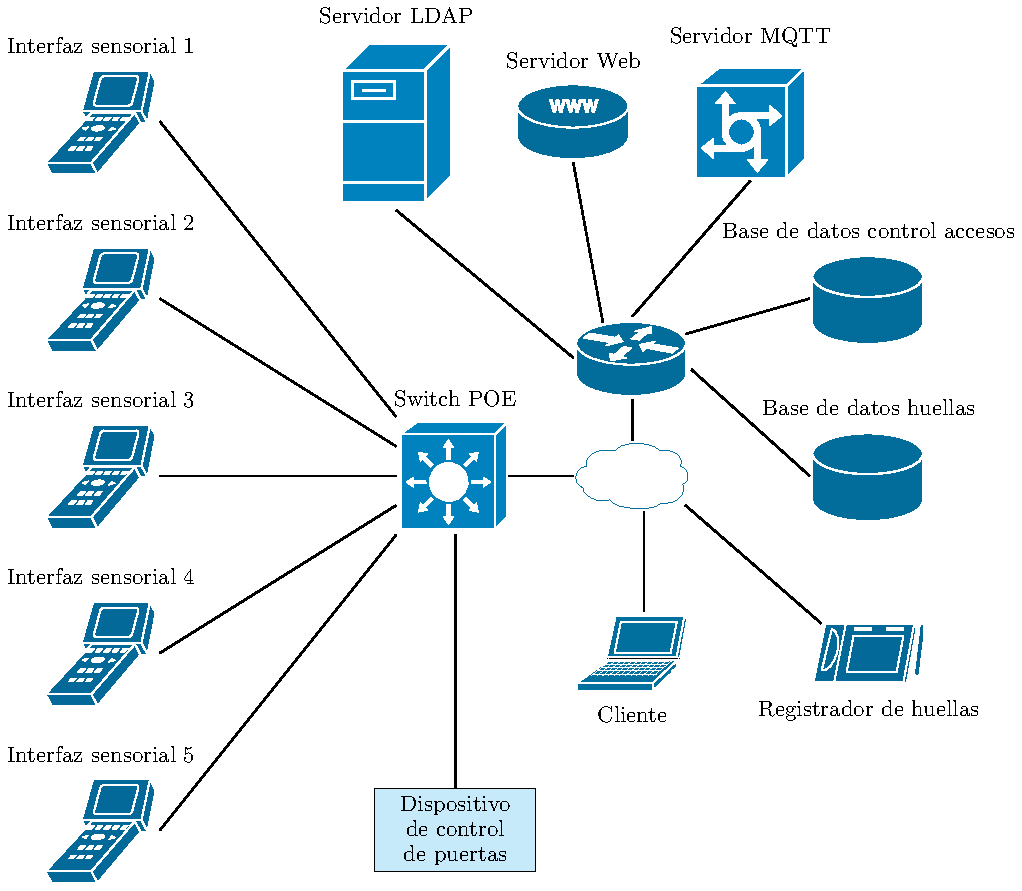
\includegraphics[width=0.95\textwidth]{topologia_red_sistema_completo.pdf}
    \caption*{\textbf{Fuente:} Elaboración propia}
    \label{fig:topologia_red_sistema_completo}
  \end{figure}  

  \begin{landscape}
    \subsection{Diagrama de flujo para el ingreso posterior a la instalación del sistema desarrollado}

    \begin{figure}[H]
      \centering
      \caption{Diagrama de flujo posterior}
      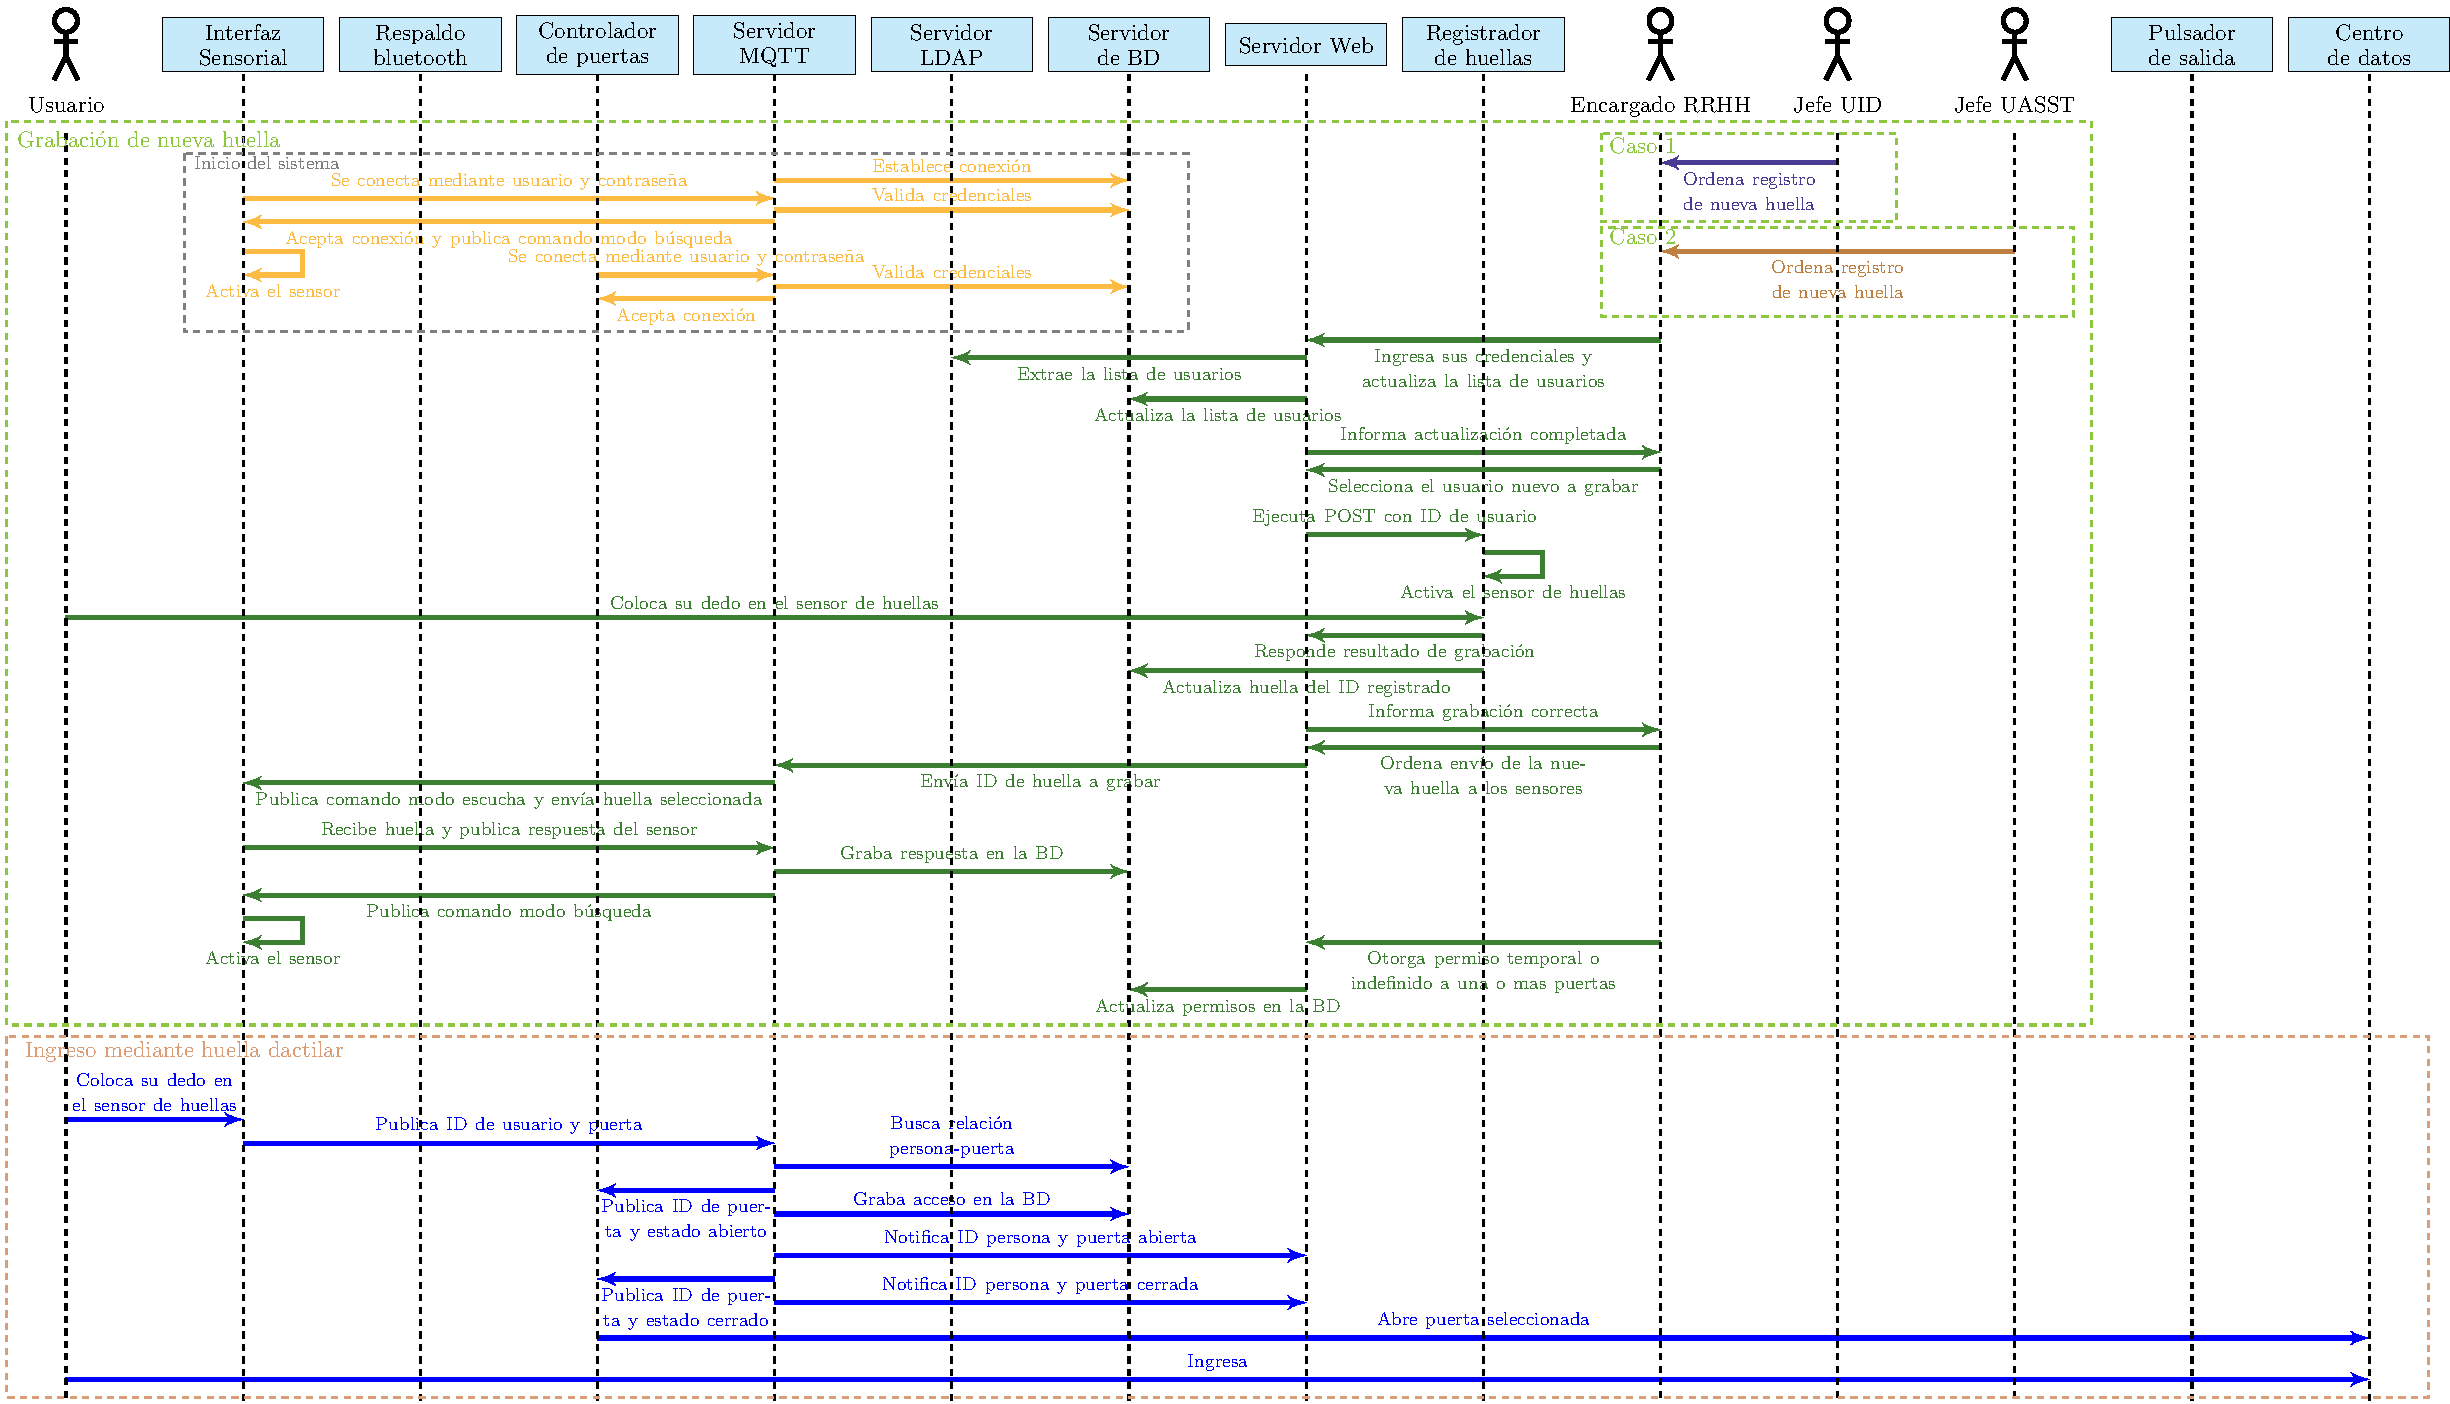
\includegraphics[width=1.393\textwidth]{flujo_ingreso_posterior_1.pdf}
      \caption*{\textbf{Fuente:} Elaboración propia. Continua en la siguiente página.}
      \label{fig:flujo_ingreso_posterior}
    \end{figure}  

    \clearpage
    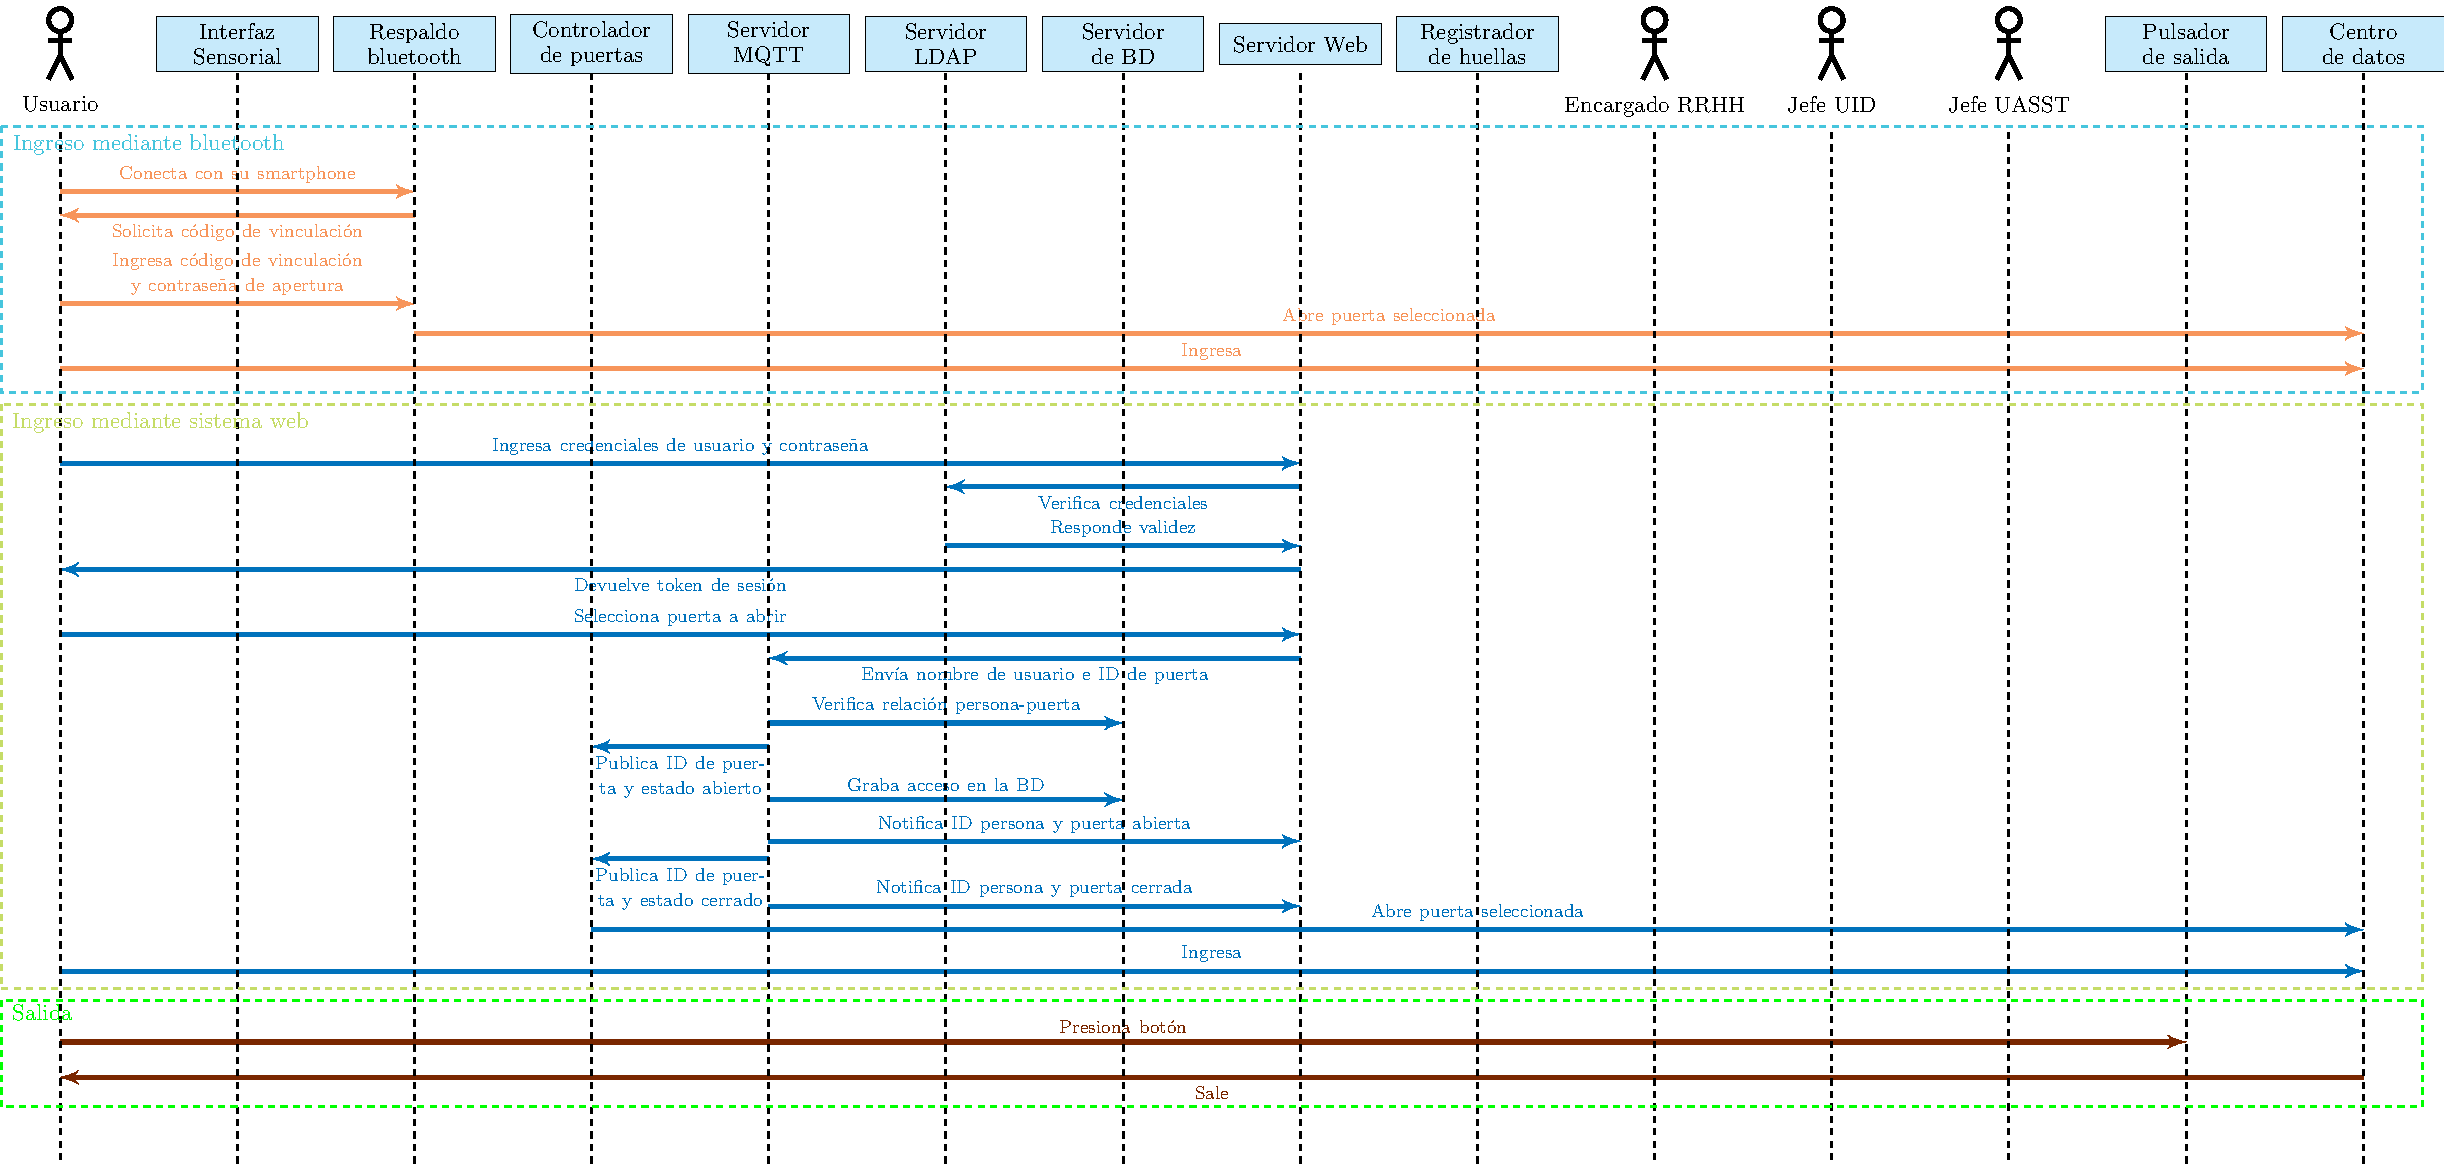
\includegraphics[width=1.393\textwidth]{flujo_ingreso_posterior_2.pdf}
    \clearpage
  \end{landscape}

  La Figura \ref{fig:flujo_ingreso_posterior} muestra el flujo de las acciones que se producen al inicio del sistema, es decir una vez que el servidor MQTT se ha encendido y el switch POE alimenta a los dispositivos de interfaz sensorial y de control de puertas, para que inicie este proceso es requisito que el servidor de bases de datos se encuentre activo.

  La grabación de huellas inicia mediante un email que recibe el encargado de recursos humanos de uno de los jefes designados por el Director Ejecutivo de ADSIB, el encargado se respalda en este correo y comienza el proceso de grabación siempre y cuando el dispositivo registrador se encuentre activo y tenga acceso a la red configurada para el sistema de control de accesos de acuerdo al diagrama de la Figura \ref{fig:topologia_red_sistema_completo}. 

  Para el ingreso al sistema web las credencias que utiliza el encargado son provistas por la persona que instaló el sistema ya que al momento de la instalación del sistema se crea un super-usuario con el que se pueden crear otros usuarios y proveerlos de permisos de administración.

  \section{Secuencia de acción para el registro de una nueva huella} \label{sec:registro_nueva_huella}

  \begin{figure}[h]
    \centering
    \caption{Diagrama de flujo para el registro de una nueva huella}
    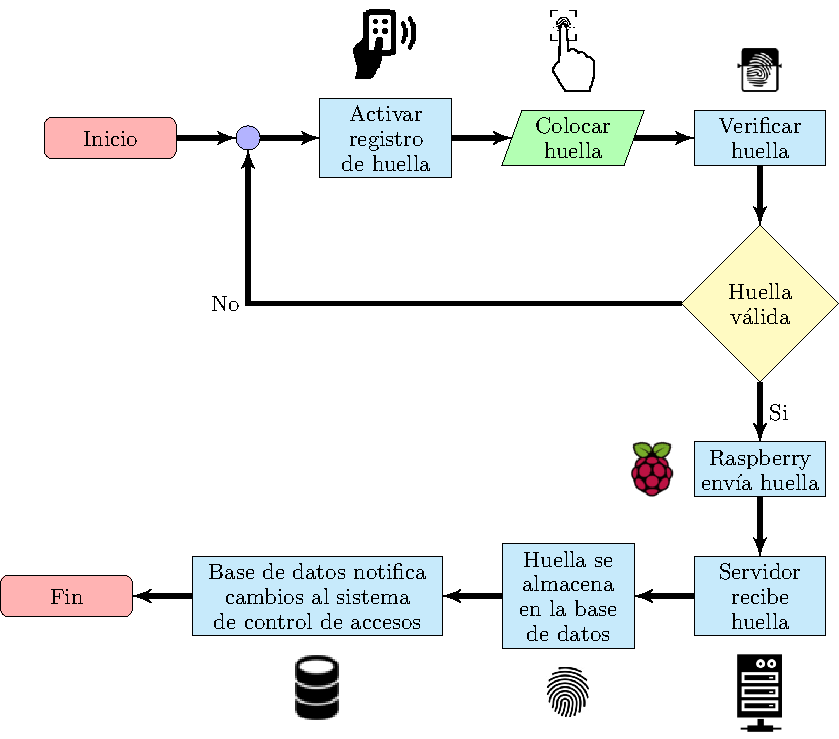
\includegraphics[width=0.95\textwidth]{flujograma_registrar_huella.pdf}
    \caption*{\textbf{Fuente:} Elaboración propia}
    \label{fig:flujo_registrador}
  \end{figure}

  Para este proceso se desarrolló un sistema basado en Raspberry Pi 3 modelo B V1.2 (aunque también es compatible Raspberry Pi 2), un sensor de huellas dactilares ZFM-20 \cite{manual:fingerprint_ZFM-20}, un módulo receptor POE para la alimentación de energía y la conexión de red.

  Este sistema se basa en la arquitectura de orquestación de micro-servicios, mediante la cual se levantan servicios particulares para cada sub-sistema; con este enfoque se observan dos micro-servicios en el lado del servidor, cuyo sistema operativo es Linux Debian 8.3, el primer micro-servicio proveé una base de datos PostgreSQL en su versión 9.4 (compatible con versiones superiores) y el segundo micro-servicio proveé una API REST en lenguaje Javascript con el manejador de rutas Express.

  \begin{figure}[h]
    \centering
    \caption{Diagrama de bloques del equipo registrador de huellas}
    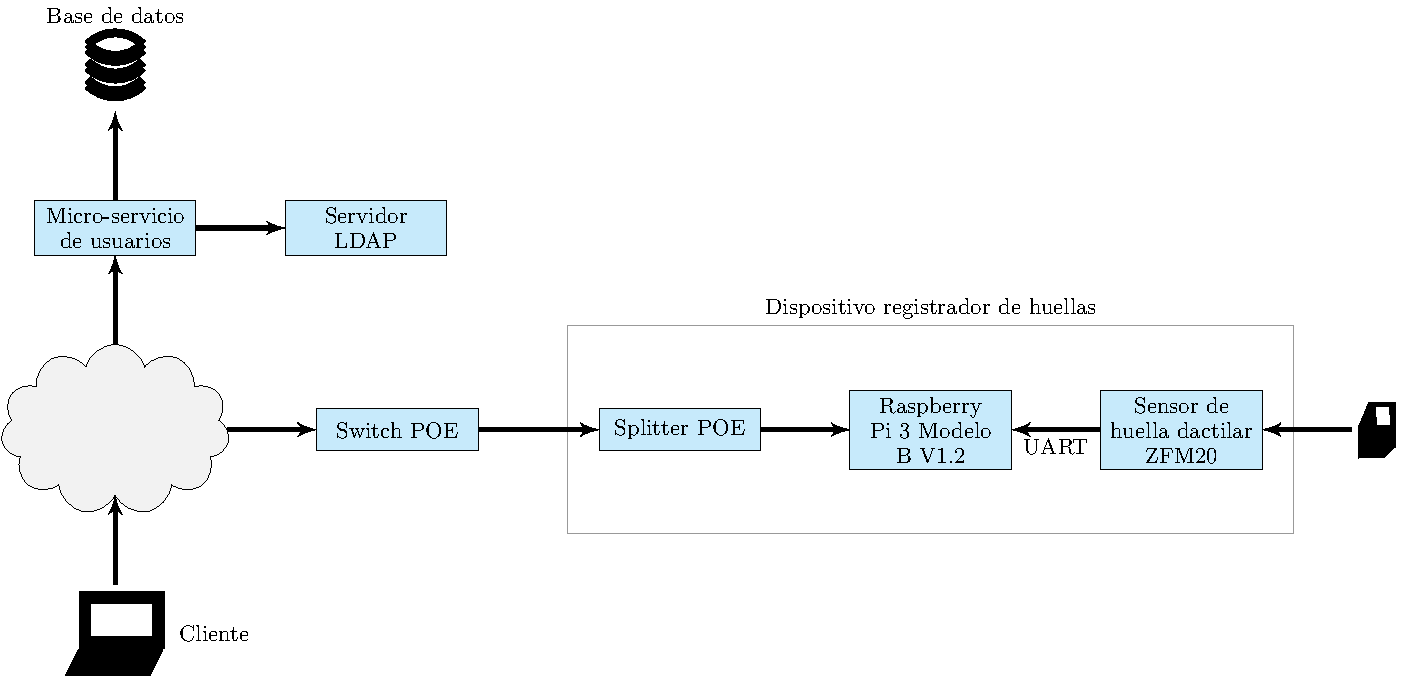
\includegraphics[width=1\textwidth]{bloques_registrador.pdf}
    \caption*{\textbf{Fuente:} Elaboración propia}
  \end{figure}

  Por otra parte el hardware embebido levanta una imagen de Linux Raspbian contenida en una tarjeta $ \mu $SD, sobre la cual se ejecutan dos micro-servicios, el primero es una API REST en Node.js con el manejador de rutas Restify que provee todos los comandos y se encarga de la comunicación con el sensor de huellas dactilares, el segundo se encarga de la sincronización de los datos de los usuarios almacenados en el servidor. Esta API es consultada por el servidor web, la comunicación se produce mediante intercambio de mensajes en formato JSON.
  
  Todos los sub-procesos son orquestados por un proceso principal que se encarga del inicio de los procesos y la transferencia de mensajes entre sub-procesos. Este proceso principal se ejecuta en el mismo servidor del broker MQTT. Todos los micro-servicios pueden ser instalados mediante la tecnología de virtualización Docker ya que el protocolo MQTT soporta la traducción de direcciones NAT\footnote{Network Address Translation}.

  \subsection{Registro de usuarios en el servidor LDAP}

  Para realizar este proceso se debe contar con un servidor OpenLDAP, el cual almacena todos los datos críticos de las personas que podrán hacer uso del sistema de puertas. El micro-servicio se conecta al servidor LDAP para obtener la lista de personas conjuntamente con sus datos adicionales como por ejemplo nombre de usuario, cargo, etc. Se pueden insertar usuarios con alguna herramienta como \href{https://wiki.debian.org/LDAP/LDAPUtils}{LDAP-utils}, \href{http://directory.apache.org/}{Apache Directory} o \href{http://phpldapadmin.sourceforge.net/wiki/index.php/Main_Page}{phpLDAPadmin}

  El servidor LDAP debe estar organizado de la siguiente manera:

  \begin{description}[align=left]
    \item[Dominio de la entidad:] dc=entidad,dc=com
    \item[Usuario administrador:] cn=admin,dc=entidad,dc=com
    \item[Grupo de usuarios:] ou=usuarios,dc=entidad,dc=com (organizational unit)
    \item[Identificador de usuario:] uid=usuario1,ou=usuarios,dc=entidad,dc=com (inetOrgPerson)
  \end{description}

  Todos los miembros \textit{(member)} que se encuentren en el grupo \textit{ou=usuarios} estarán disponibles para poder acceder por las puertas de acuerdo a la tabla de \textit{permisos} que se mostrará mas adelante.

  Los datos adicionales que se utilizarán para cada usuario son los siguientes:

  \begin{description}[align=left]
    \item[Nombres:] givenName=Jhon Juan
    \item[Apellidos:] sn=Doe Pérez
    \item[Carnet de identidad:] cn=5552368
    \item[Cargo:] title=Encargado de recursos humanos
    \item[Tipo de cargo:] employeeType=rrhh
    \item[Clave:] userPassword=abc123
    \item[Correo:] mail=jhon@doe.com
    \item[Teléfono:] telephoneNumber=5550123
  \end{description}

  El tipo de cargo se puede utilizar para brindar permisos de administración del sistema solo a ciertos tipos de cargos.

  Si el servidor LDAP se vá a utilizar para la autenticación de usuarios en otros servicios como correos electrónicos, almacenamiento en la nube, etc, es muy recomendable cifrar la comunicación mediante SSL.

  \begin{figure}[H]
    \centering
    \caption{Registro de usuario en el servidor de LDAP}
    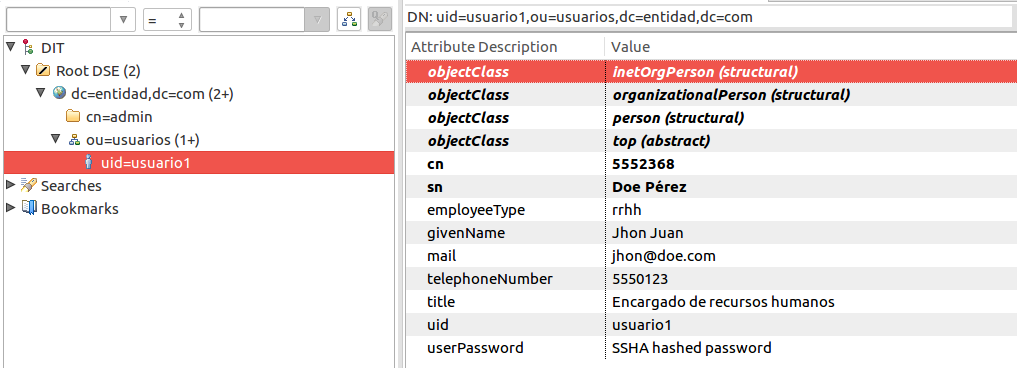
\includegraphics[width=1\textwidth]{ingenieria_proyecto/captura_ldap_usuario.png}
    \caption*{\textbf{Fuente:} Elaboración propia}
  \end{figure}

  \subsection{Base de datos de huellas}

  Esta base de datos se sincroniza con los datos del servidor LDAP mediante el micro-servicio de usuarios, dentro está contenida la lista de personas, sus huellas y la imagen de sus huellas.

  Existe una relación 1-1 entre el campo id de la tabla \textit{huella} que toma de referencia el ID de la tabla \textit{personas}, la plantilla de cada huella es un número hexadecimal de 512 bytes en formato de cadena de caracteres, tal como se indica en la sección de \textit{Character file buffer} del manual del sensor ZFM-20 \cite{manual:fingerprint_ZFM-20}.

  Del mismo modo, la imagen de cada huella es un número hexadecimal de 36864 bytes en formato de cadena de caracteres, tal como se indica en la sección de \textit{Image file buffer} del manual del sensor ZFM-20 \cite{manual:fingerprint_ZFM-20}. Este número necesita un tratamiento antes de representarlo como una imagen ya que el sensor solo envía el nibble más alto de cada pixel, por lo cual cada nibble debe desplazarse cuatro posiciones a la izquierda, con lo que se obtendría un número de 73728 bytes, los cuales se deben acomodar en una matriz de $ 288 x 256 $ para formar la imagen en formato de mapa de bits de escala de grises de cada huella.

  \begin{figure}[H]
    \centering
    \caption{Imagen de huella generada desde el sensor ZhianTec ZFM-20}
    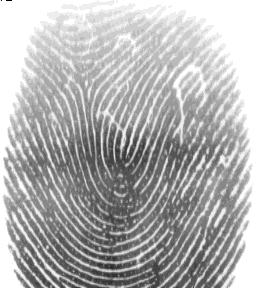
\includegraphics[width=0.2\textwidth]{ingenieria_proyecto/huella_sensor.png}
    \caption*{\textbf{Fuente:} Elaboración propia}
  \end{figure}
  
  \subsubsection{Forma normal 1 para la base de datos de huellas}

  La reducción de esta base de datos solo necesita de la Forma Normal 1 para eliminar los datos repetidos, eliminar errores lógicos y tener los datos ordenados. Los datos de prueba se observan el la Tabla \ref{tab:base_datos_huellas}.

  \begin{table}[H]
    \centering
    \caption{Datos de prueba para la base de datos de huellas}
    \begin{tabular}{|C{3cm}|C{3cm}|C{3cm}|}
  \hline
  \rowcolor[HTML]{E3FFE3}
  usuario & huella\_imagen & huella\_plantilla \\
  \hline
  jdoe & 8abddeeeefff... & 03014e138d00... \\
  \hline
  jperez & 21cff04631dc... & 8647a9cdf8a1... \\
  \hline
\end{tabular}

    \caption*{\textbf{Fuente:} Elaboración propia}
    \label{tab:base_datos_huellas}
  \end{table}

  Con la reducción de la Tabla \ref{tab:base_datos_huellas_fn1} se obtiene el diagrama entidad-relación de la Figura \ref{fig:base_datos_huellas_diagrama}.

  \begin{table}[H]
    \caption{Reducción a la Forma Normal 1 de la base de datos de huellas}
    \begin{subtable}{\linewidth}
      \centering
      \caption{Tabla persona}
      \begin{tabular}{|C{3cm}|C{3cm}|}
  \hline
  \rowcolor[HTML]{E3FFE3}
  id & usuario \\
  \hline
  1 & jdoe \\
  \hline
  2 & jperez \\
  \hline
\end{tabular}
    \end{subtable}
    \begin{subtable}{\linewidth}
      \centering
      \caption{Tabla huella}
      \begin{tabular}{|C{3cm}|C{3cm}|C{3cm}|}
  \hline
  \rowcolor[HTML]{E3FFE3}
  id & imagen & plantilla \\
  \hline
  1 & 8abddeeeefff... & 03014e138d00... \\
  \hline
  2 & 21cff04631dc... & 8647a9cdf8a1... \\
  \hline
\end{tabular}
    \end{subtable} 
    \caption*{\textbf{Fuente:} Elaboración propia}
    \label{tab:base_datos_huellas_fn1}
  \end{table}

  \begin{figure}[H]
    \centering
    \caption{Diagrama entidad-relación para la base de datos de huellas}
    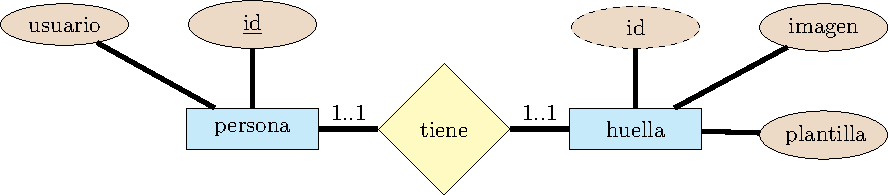
\includegraphics[width=0.8\textwidth]{base_datos_huellas_diagrama.pdf}
    \caption*{\textbf{Fuente:} Elaboración propia}
    \label{fig:base_datos_huellas_diagrama}
  \end{figure}

  Lo cual finalmente genera la base de datos mostrada en la Figura \ref{fig:bd_huellas}.

  \begin{figure}[H]
    \centering
    \caption{Base de datos de huellas}
    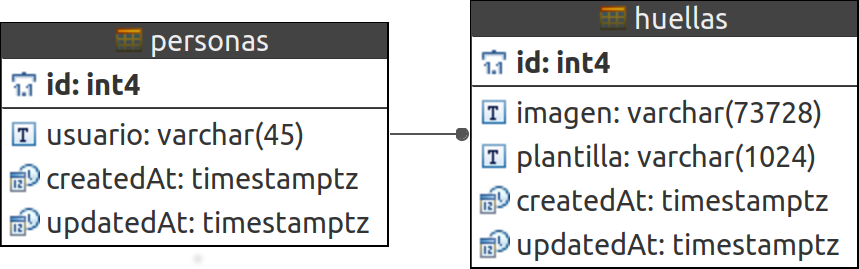
\includegraphics[width=0.6\textwidth]{ingenieria_proyecto/bd_huellas.png}
    \caption*{\textbf{Fuente:} Elaboración propia}
    \label{fig:bd_huellas}
  \end{figure}

  \subsection{Hardware registrador de huellas}

  Este hardware se compone de los siguientes componentes:
  \begin{description}[align=left]
    \item[Splitter POE:] Este equipo sirve para separar los datos de la energía que viajan juntos por la conexión Ethernet, se conecta la salida de datos a la entrada RJ-45 del Raspberry y se alimenta a todo el equipo con la energía recibida por el POE, dado que éste puede alcanzar hasta los 12.95W en el estándar 802.3af y el equipo completo consume como pico máximo 3.65W (Incluyendo el splitter mismo), se observa que este estándar es suficiente para alimentar el dispositivo.
    \item[Raspberry:] Es el computador donde se realizan todos los procesos de captura de huellas y sincronización de la base de datos con el servidor LDAP.
    \item[Sensor dactilar ZFM-20:] Es el módulo que se conecta mediante UART y se alimenta desde el GPIO del Raspberry.
  \end{description}

  \begin{figure}[h]
    \centering
    \caption{Prototipo del hardware grabador de huellas}
    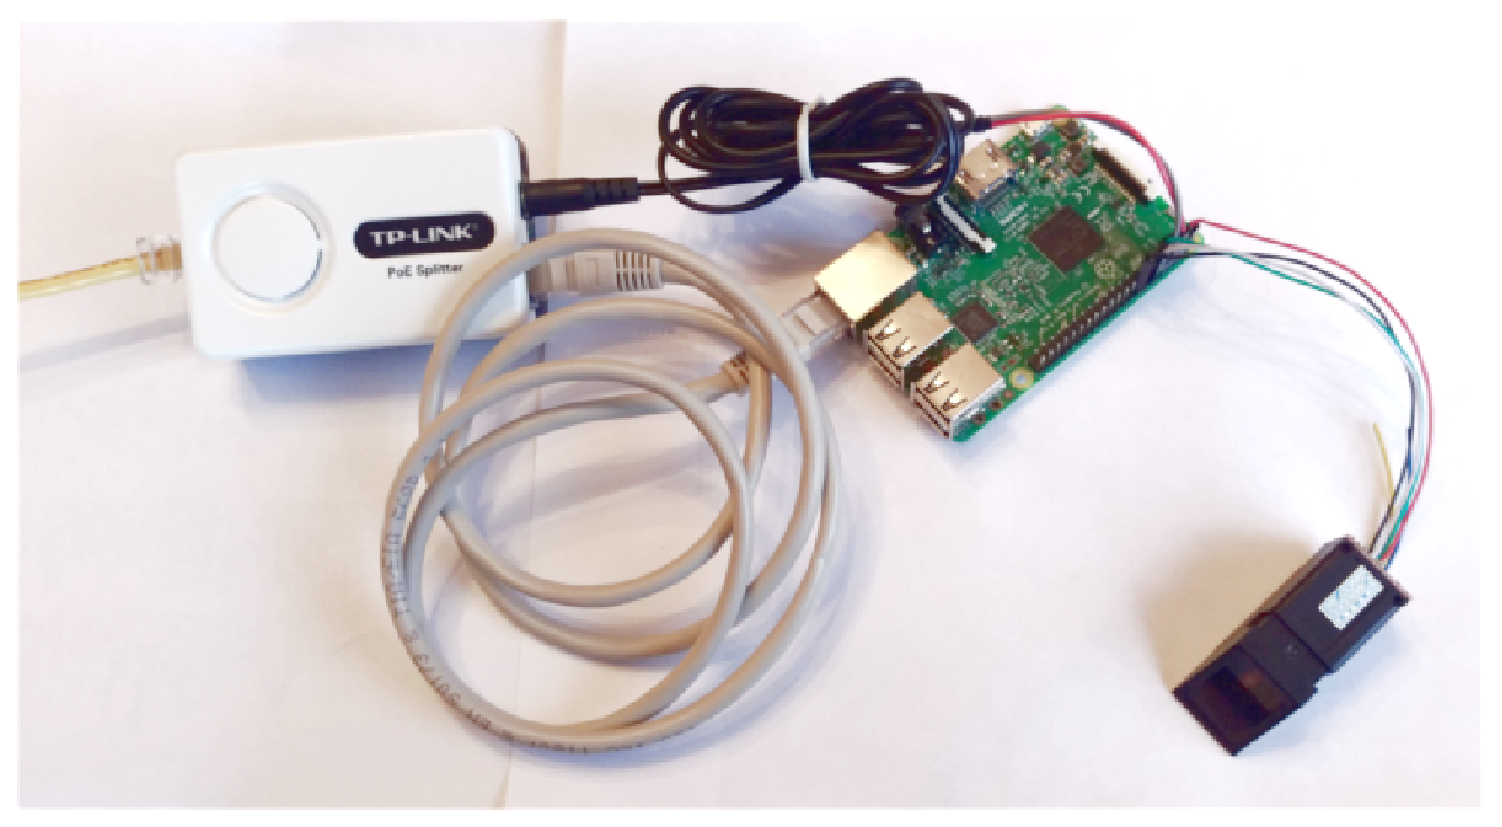
\includegraphics[width=0.9\textwidth]{ingenieria_proyecto/foto_registrador_huellas.eps}
    \caption*{\textbf{Fuente:} Elaboración propia}
    \label{fig:prototipo_registrador}
  \end{figure}

  Para realizar la validación de alimentación de energía mediante POE se debe calcular la potencia del equipo que se desea energizar, para ello se calcula la potencia consumida por cada dispositivo al extremo receptor de la línea de POE. En este caso tenemos 3 equipos a alimentar, los datos para este efecto fueron obtenidos de la hoja de datos del Splitter POE \cite{datasheet:TL-POE10R_V4}, la hoja de datos del Sensor de huella dactilar \cite{manual:fingerprint_ZFM-20} y la tabla de consumo de energía de \href{https://www.pidramble.com/wiki/benchmarks/power-consumption}{Rasbperry Pi Dramble}\footnote{\href{https://www.pidramble.com/wiki/benchmarks/power-consumption}{https://www.pidramble.com}}.

  En corriente continua la potencia eléctrica desarrollada por un dispositivo entre dos terminales, es el producto de la diferencia de potencial entre las dos terminales y la intensidad de corriente que circula por el dispositivo:

  \vspace{-1.5em}
  \begin{equation}
    \label{calculo_potencia}
    P = \frac{dw}{dt} = \frac{dw}{dq} \cdot \frac{dq}{dt} = V \cdot I
  \end{equation}
  \vspace{-2em}

  Donde: V es el valor instantáneo del voltaje expresado en Voltios, I es el valor instantáneo de la intensidad de corriente expresado en Amperios y P es el valor instantáneo de la potencia expresado en Vatios.

  \begin{table}[H]
    \centering
    \caption{Cálculo de potencia consumida por cada dispositivo capturador de huellas}
    \begin{tabular}{|C{2.5cm}|C{2.5cm}|C{2.5cm}|C{2.5cm}|C{2.5cm}|}
  \hline
  \rowcolor[HTML]{E3FFE3} Dispositivo & Modelo & Voltaje de alimentación & Consumo de corriente & Potencia consumida \\
  \hline
  Splitter POE & TL-POE10R & 12V & 80mA & 0.96W \\
  \hline
  Raspberry Pi & 3 B V1.2  & 5V & 480mA & 2.40W \\
  \hline
  Sensor de huella dactilar & ZFM-20 & 5V & 150mA & 0.75W \\
  \hline
  \multicolumn{4}{|c|}{Total} & 4.11W \\
  \hline
\end{tabular}
    \caption*{\textbf{Fuente:} Elaboración propia}
  \end{table}

  Este resultado se adhiere a los parámetros de la instalación, como por ejemplo la longitud máxima del segmento de par trenzado UTP, el número de dispositivos a alimentar, el estándar a utilizar y el voltaje provisto desde el extremo inyector de la línea de POE.

  \begin{table}[H]
    \centering
    \caption{Parámetros para el cálculo de potencia consumida del capturador de huellas}
    \begin{tabular}{|r|c|}
  \hline
  \rowcolor[HTML]{E3FFE3} \multicolumn{1}{|c|}{Parámetro} & Valor \\
  \hline
  Estándar POE & 802.3af \\
  \hline
  Distancia & 100m \\
  \hline
  Voltaje de alimentación & 48V \\
  \hline
  Watts requeridos & 4.11W \\
  \hline
  Número de dispositivos para alimentar & 1 \\
  \hline
\end{tabular}
    \caption*{\textbf{Fuente:} Elaboración propia}
  \end{table}

  Con todos estos datos se puede realizar el cálculo de la potencia real que debe suministrarse desde el inyector de la línea de POE, ya que a lo largo de la línea se producen pérdidas por la resistencia eléctrica del par trenzado. Muchas veces éste es un problema que no es considerado, por lo cual si no se contempló este cálculo al realizar la instalación, los equipos podrían funcionar incorrectamente o definitivamente podrían no funcionar.

  El cable UTP previsto para los cálculos es de categoría 5e, de aleación cobre/aluminio al 10\%, de medida 28AWG cuya resistencia es de 101$ \Omega $ para una longitud de 1000 pies. [Anexo \ref{anx:resistencia_cable_cobre}]

  Mediante la herramienta de cálculos para diseños de red POE \href{http://poe-texas.com/Calculator/}{POE-Texas Calculator}\footnote{\href{http://poe-texas.com/Calculator/}{http://poe-texas.com/Calculator/}} y los parámetros mostrados anteriormente se obtiene la pérdida de energía en la línea de transmisión POE y la potencia real que debe ser suministrada en el extremo inyector de la línea.

  \begin{table}[H]
    \caption{Potencia consumida por el dispositivo registrador de huellas al extremo receptor POE}
    \centering
    \begin{tabular}{|r|c|}
  \hline
  \rowcolor[HTML]{E3FFE3} 
  \multicolumn{1}{|c|}{\cellcolor[HTML]{E3FFE3}Parámetro} & Valor      \\ \hline
  Voltaje al extremo del tramo                            & 47.27V     \\ \hline
  Corriente al extremo del tramo                          & 90mA       \\ \hline
  Resistencia del cable                                   & 8.3968$ \Omega $ \\ \hline
  Pérdida de potencia en la línea                         & 0.06W      \\ \hline
  Potencia suministrada desde el inyector                 & 4.17W      \\ \hline
\end{tabular}
    \caption*{\textbf{Fuente:} Elaboración propia}
  \end{table}

  \section{Secuencia de acción para el acceso mediante sensor biométrico de huellas dactilares}

  Antes de ejecutar este proceso se debe registrar la huella de las personas que ingresarán a los ambientes resguardados por el sistema tal como se menciona en la Sección \ref{sec:registro_nueva_huella}, caso contrario el sistema no reconocerá una huella conocida y este proceso se truncará en el primer paso.

  También se debe tener la certeza de que los dispositivos pueden acceder al servidor MQTT mediante una infraestructura de red como la que se muestra en la Figura \ref{fig:topologia_red_sistema_completo}, en caso de existir un router, éste debe contar con las reglas necesarias para permitir el envío y recepción de paquetes HTTP e ICMP\footnote{Internet Control Message Protocol} desde y hacia el servidor MQTT.

  Se debe verificar que los dispositivos se encuentren alimentados por el switch POE y no exista ningún tipo de alerta en el mismo.

  \begin{figure}[H]
    \centering
    \caption{Diagrama de flujo para la apertura de puerta mediante biométrico}
    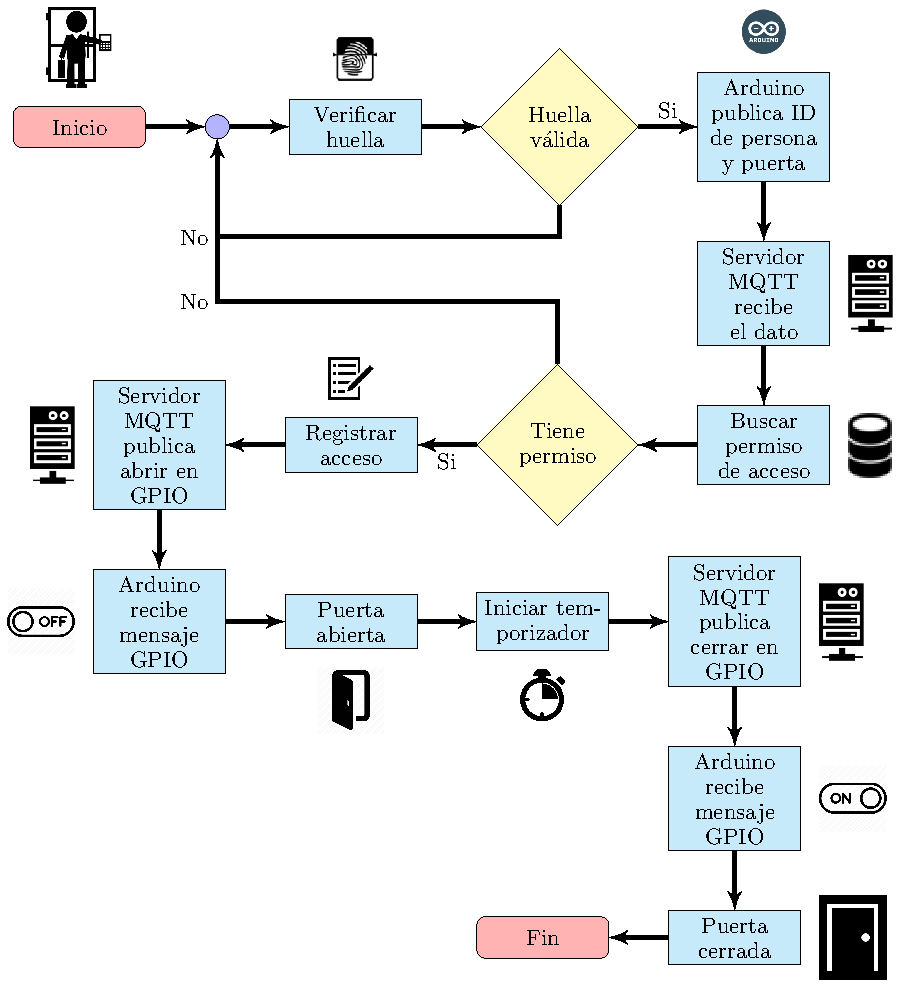
\includegraphics[width=1\textwidth]{flujograma_nuevo_acceso.pdf}
    \caption*{\textbf{Fuente:} Elaboración propia}
    \label{fig:flujo_acceso_biometrico}
  \end{figure}

  \subsection{Hardware de control e interfaz sensorial}

  El diseño de este hardware se realizó en base al esquema de Arduino UNO R3, al cual se habilita una conexión de red mediante el circuito integrado ENC28J60 y ambos bloques son alimentados mediante POE gracias al circuito integrado LTC4267-3, el esquema de la placa desarrollada se puede observar en el Anexo \ref{anx:esquema_placa_poe}.

  Este dispositivo se utiliza tanto para realizar la conexión con el sensor de huellas dactilares como para realizar el control de los actuadores que abren y cierran las puertas, ambos se conectan al sistema mediante el protocolo MQTT como se puede observar en el siguiente diagrama:

  \begin{figure}[H]
    \centering
    \caption{Diagrama de bloques de los dispositivos de control e interfaz sensorial}
    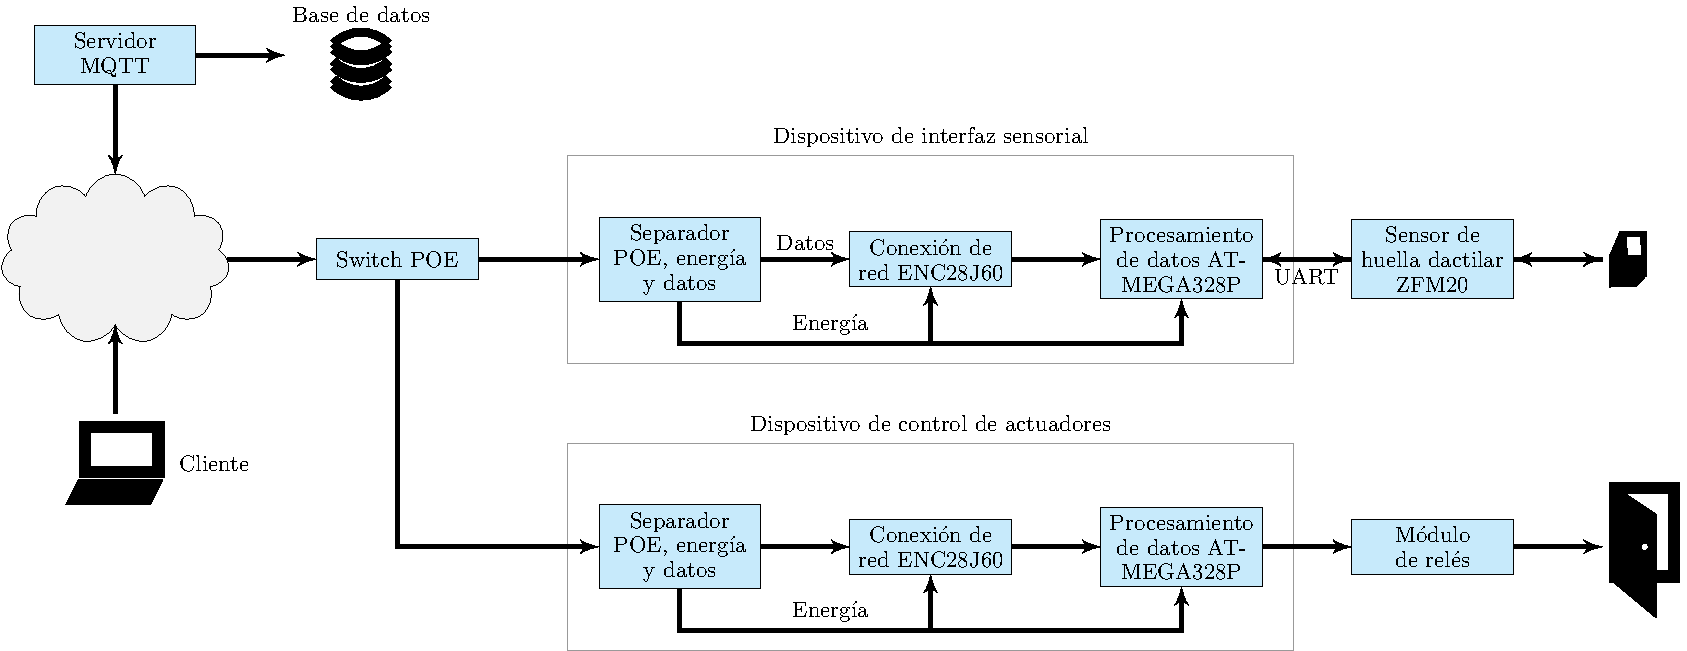
\includegraphics[width=1\textwidth]{bloques_interfaz_sensorial.pdf}
    \caption*{\textbf{Fuente:} Elaboración propia}
  \end{figure}

  \subsubsection{Separador POE, energía y datos}

  Esta etapa se encarga de negociar la potencia requerida para alimentar el circuito de interfaz sensorial o de control de actuadores, se basa en el esquema de Splitter POE diseñado por Linear Technology [Anexo \ref{anx:esquematico_POE_LTC4267}], cuyo componente central es el circuito integrado LTC4267-3, que se encarga de negociar la energía provista por el inyector.

  \begin{figure}[H]
    \centering
    \caption{Diagrama de bloques del Splitter POE}
    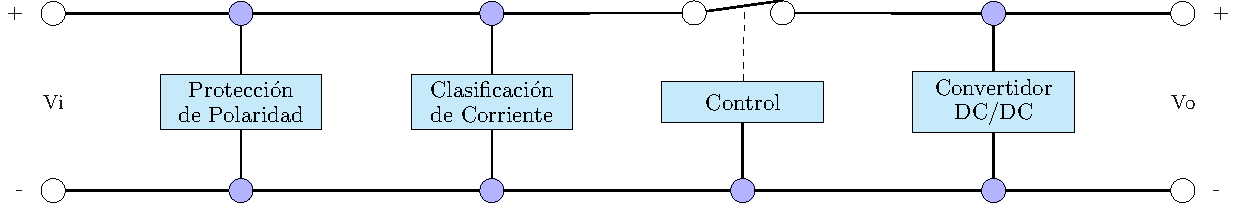
\includegraphics[width=1\textwidth]{bloques_funcionamiento_poe.pdf}
    \caption*{\textbf{Fuente:} Elaboración propia}
  \end{figure}

  El primer bloque del circuito POE es el de Protección de Polaridad, la tensión desde el inyector puede venir de dos formas, una es utilizar dos pares alternativos del cable ethernet para enviar el voltaje positivo en uno y el negativo en otro. La segunda forma es enviar la tensión conjuntamente con los datos, ésta forma tiene la ventaja de que los pares alternativos se pueden utilizar para llegar a la velocidad de 1Gigabit mientras que la primera forma solo alcanza los 10/100Megabits.

  \begin{table}[H]
    \caption{Estándares 802.3af A y B, perspectiva desde el inyector}
    \centering
    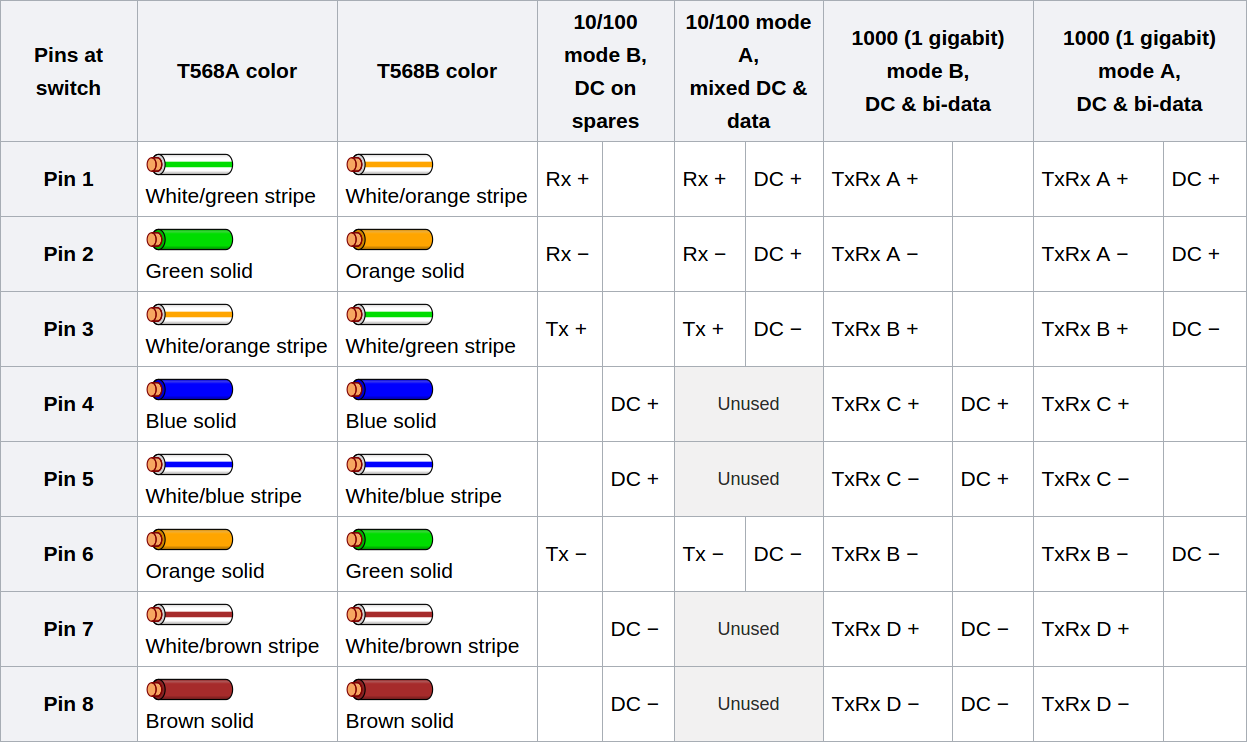
\includegraphics[width=1\textwidth]{ingenieria_proyecto/estandares_A_B_inyector_poe.png}
    \caption*{\textbf{Fuente:} \href{https://en.wikipedia.org/wiki/Power_over_Ethernet}{Power Over Ethernet, Pinouts, Wikipedia}}
  \end{table}

  El segundo bloque del circuito POE es el de Clasificación de Corriente, existen 4 fases durante la etapa de negociación, la primera es para verificar si el equipo al extremo receptor es o no POE, para ello el inyector aplicará una tensión de 2.7V a 10V buscando una resistencia de 25$ K\Omega $. Si ésta es demasiado baja o alta no continuará aplicando tensión.

  En caso de que el dispositivo sí sea POE, la tensión se eleva de 14.5V a 20.5V y se mide la corriente que circula por el receptor, con este resultado el inyector determina cual es la tensión máxima permitida para el funcionamiento del dispositivo POE.

  La tercera etapa es el comienzo de la alimentación del dispositivo y en la cuarta etapa se tiene una tensión constante para el funcionamiento continuo del dispositivo POE.

  El tercer bloque del circuito POE es el de Control, en esta fase se tiene un convertidor DC/DC \cite{datasheet:ep10} que se mantendrá apagado hasta que se haya terminado la etapa de clasificación, es decir cuando el voltaje haya alcanzado los 35V.

  El cuarto bloque es la activación del convertidor DC/DC, es el paso final para la alimentación del circuito POE, es aquí donde se reduce la tensión DC de 48V a la tensión necesaria para el funcionamiento del circuito.

  \subsubsection{Conexión de red ENC28J60}

  Esta etapa se basa en el esquema de la placa Olimex Ethercard [Anexo \ref{anx:esquematico_ethercard}], cuyo componente central es el circuito integrado ENC28J60, este dispositivo tiene 6 registros en su mapa de registros de control que definen la dirección MAC al momento de realizar la conexión con el microcontrolador mediante el protocolo SPI. Precisa de un oscilador a 25MHz además de una alimentación de 3.3V, pero se debe tomar en cuenta que la comunicación SPI se realiza al nivel TTL de 5V.

  Se le puede definir una IP estática pero también tiene soporte para la asignación de IP por DHCP, soporta las operaciones de Capa 3 o Capa de Red del Modelo OSI. Cabe mencionar que este circuito brinda soporte para trabajar a 10/100MBits, pero para este proyecto no es necesaria una conexión más veloz, por lo cual el bajo costo del dispositivo justifica esta velocidad.

  Es mediante este circuito integrado que todos los datos son enviados y recibidos desde el servidor MQTT hasta el microcontrolador para que puedan ser procesados de manera adecuada. Para comunicar el microcontrolador con este circuito se utilizó la librería UIP Ethernet\footnote{\href{https://github.com/ntruchsess/arduino_uip}{github.com/ntruchsess/arduino\_uip}} compatible con Arduino. Mediante la cual se levanta un cliente MQTT con una dirección IP y MAC estáticas, mismas que son almacenadas en la base de datos para permitir o rechazar la conexión en el lado del servidor.

  \subsubsection*{Circuito de interfaz sensorial}

  Cuando una persona coloca su dedo en un sensor de huellas, este sensor busca en su base de datos interna si la huella está registrada, si no está no realiza ningún proceso, pero si la huella se encuentra en su base de datos envía el id al circuito de interfaz sensorial; este lo reenvía hacia el servidor MQTT con el tópico \textit{p} seguido del id de la puerta, y el contenido del mensaje es el id obtenido del sensor:

  \begin{center}
    p/:idPuerta \quad $ \rightarrow $ \quad :idPersona
  \end{center}

  El servidor MQTT recibe el mensaje y busca si el ID de la persona tiene permiso de acceso temporal o indefinido por el ID de la puerta; en caso de que la persona no tenga acceso el servidor no responde nada, pero si la persona tiene permiso de acceso el servidor envía un mensaje al circuito de control que se encarga de la apertura de dicha puerta.

  \begin{figure}[h]
    \centering
    \caption{Prototipo del circuito de interfaz sensorial}
    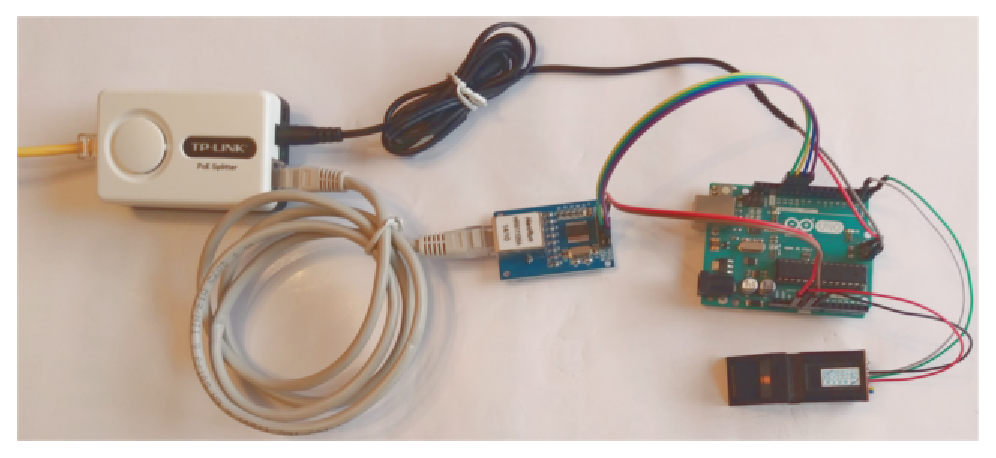
\includegraphics[width=1\textwidth]{ingenieria_proyecto/foto_interfaz_sensorial.eps}
    \caption*{\textbf{Fuente:} Elaboración propia}
  \end{figure}

  En cuanto al consumo de energía del circuito de interfaz sensorial se realizan los cálculos en base a la ecuación \ref{calculo_potencia}.

  \begin{table}[H]
    \centering
    \caption{Cálculo de potencia consumida por cada dispositivo interfaz sensorial}
    \begin{tabular}{|C{2.5cm}|C{2.5cm}|C{2.5cm}|C{2.5cm}|C{2.5cm}|}
  \hline
  \rowcolor[HTML]{E3FFE3} Dispositivo & Modelo & Voltaje de alimentación & Consumo de corriente & Potencia consumida \\
  \hline
  Hardware diseñado & Interfaz Sensorial & 5V & 200mA & 1W \\
  \hline
  Sensor de huella dactilar & ZFM-20 & 5V & 150mA & 0.75W \\
  \hline
  \multicolumn{4}{|c|}{Total} & 1.75W \\
  \hline
\end{tabular}
    \caption*{\textbf{Fuente:} Elaboración propia}
  \end{table}

  Este valor se añade a los parámetros de instalación de cada puerta por donde se desea acceder mediante la huella dactilar.

  \begin{table}[H]
    \centering
    \caption{Parámetros para el cálculo de potencia consumida por la interfaz sensorial}
    \begin{tabular}{|r|c|}
  \hline
  \rowcolor[HTML]{E3FFE3} \multicolumn{1}{|c|}{Parámetro} & Valor \\
  \hline
  Estándar POE & 802.3af \\
  \hline
  Distancia & 100m \\
  \hline
  Voltaje de alimentación & 48V \\
  \hline
  Watts requeridos & 1.75W \\
  \hline
  Número de dispositivos para alimentar & 1 \\
  \hline
\end{tabular}
    \caption*{\textbf{Fuente:} Elaboración propia}
  \end{table}

  Con un par trenzado UTP categoría 5e, mediante la herramienta de cálculos para diseños de red POE \href{http://poe-texas.com/Calculator/}{POE-Texas Calculator}\footnote{\href{http://poe-texas.com/Calculator/}{http://poe-texas.com/Calculator/}} se obtiene la pérdida en la línea.

  \begin{table}[H]
    \caption{Potencia consumida por el dispositivo interfaz sensorial al extremo receptor POE}
    \centering
    \begin{tabular}{|r|c|}
  \hline
  \rowcolor[HTML]{E3FFE3} 
  \multicolumn{1}{|c|}{\cellcolor[HTML]{E3FFE3}Parámetro} & Valor \\
  \hline
  Voltaje al extremo del tramo & 47.69V \\
  \hline
  Corriente al extremo del tramo & 40mA \\
  \hline
  Resistencia del cable & 8.3968$ \Omega $ \\
  \hline
  Pérdida de potencia en la línea & 0.01W \\
  \hline
  Potencia suministrada desde el inyector & 1.76W \\
  \hline
\end{tabular}
    \caption*{\textbf{Fuente:} Elaboración propia}
  \end{table}

  \subsubsection*{Circuito de control de actuadores}

  Una vez que el servidor MQTT determinó que una persona tiene acceso por una puerta, envía un mensaje en el siguiente formato:

  \begin{center}
    gpio/:idDispositivoControl/:pin \quad $ \rightarrow $ \quad :estado
  \end{center}

  Donde el \textit{idDispositivoControl} identifica el ID del dispositivo que controla la puerta que se desea abrir, el \textit{pin} es la salida digital que está conectada al relé de la puerta y el \textit{estado} puede ser 0 o 1, para abrir o cerrar la puerta.

  \begin{figure}[h]
    \centering
    \caption{Prototipo del circuito de control de actuadores}
    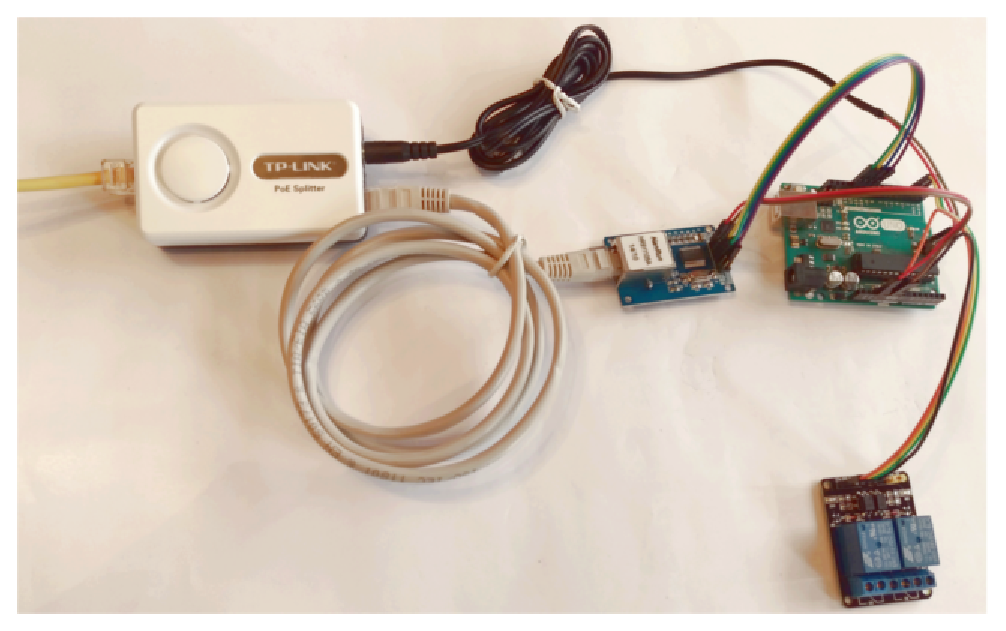
\includegraphics[width=1\textwidth]{ingenieria_proyecto/foto_control_reles.eps}
    \caption*{\textbf{Fuente:} Elaboración propia}
  \end{figure}

  Se ha determinado un tiempo de 6 segundos entre el envío de un mensaje de apertura de una puerta y el mensaje de cierre, dado que este tiempo es suficiente para que la persona pueda abrir la puerta e ingresar al recinto antes de que la puerta vuelva a cerrarse.

  Como se mencionó antes, este dispositivo tiene conectado un módulo de relés que conectan el pin de control de cada cerradura magnética a tierra cuando reciben un impulso 0 lógico a la entrada, con lo que el pistón de la cerradura cambia de posición y deja la puerta abierta \cite{datasheet:chapa_tesa}.

  \begin{figure}[H]
    \centering
    \caption{Conexión de las cerraduras electromagnéticas}
    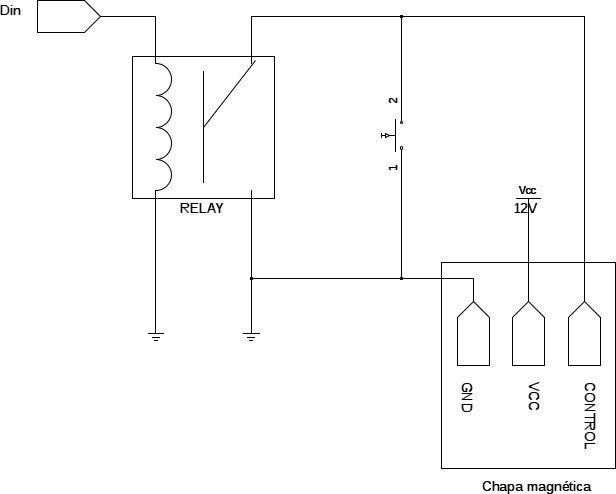
\includegraphics[width=0.55\textwidth]{ingenieria_proyecto/conexion_puerta.png}
    \caption*{\textbf{Fuente:} Elaboración propia}
    \label{fig:conexion_puerta}
  \end{figure}

  Para el dispositivo de control de puertas también se realizan los cálculos en base a la ecuación \ref{calculo_potencia}.

  \begin{table}[H]
    \centering
    \caption{Cálculo de potencia consumida por cada dispositivo de control}
    \begin{tabular}{|C{2.5cm}|C{2.5cm}|C{2.5cm}|C{2.5cm}|C{2.5cm}|}
  \hline
  \rowcolor[HTML]{E3FFE3} Dispositivo & Modelo & Voltaje de alimentación & Consumo de corriente & Potencia consumida \\
  \hline
  Hardware diseñado & Dispositivo de control & 5V & 200mA & 1W \\
  \hline
  Módulo relé & 4 canales & 5V & 470mA & 2.35W \\
  \hline
  \multicolumn{4}{|c|}{Total} & 3.35W \\
  \hline
\end{tabular}
    \caption*{\textbf{Fuente:} Elaboración propia}
  \end{table}

  Este valor se añade a los parámetros de instalación de cada puerta por donde se desea acceder mediante la huella dactilar.

  \begin{table}[H]
    \centering
    \caption{Parámetros para el cálculo de potencia consumida por la placa de control}
    \begin{tabular}{|r|c|}
  \hline
  \rowcolor[HTML]{E3FFE3} \multicolumn{1}{|c|}{Parámetro} & Valor \\
  \hline
  Estándar POE & 802.3af \\
  \hline
  Distancia & 100m \\
  \hline
  Voltaje de alimentación & 48V \\
  \hline
  Watts requeridos & 3.35W \\
  \hline
  Número de dispositivos para alimentar & 1 \\
  \hline
\end{tabular}
    \caption*{\textbf{Fuente:} Elaboración propia}
  \end{table}

  Tomando como referencia el cable par trenzado UTP categoría 5e, mediante la herramienta de cálculos para diseños de red POE \href{http://poe-texas.com/Calculator/}{POE-Texas Calculator}\footnote{\href{http://poe-texas.com/Calculator/}{http://poe-texas.com/Calculator/}} se obtiene la pérdida en la línea.

  \begin{table}[H]
    \caption{Potencia consumida por la placa de control al extremo receptor POE}
    \centering
    \begin{tabular}{|r|c|}
  \hline
  \rowcolor[HTML]{E3FFE3} 
  \multicolumn{1}{|c|}{\cellcolor[HTML]{E3FFE3}Parámetro} & Valor \\
  \hline
  Voltaje al extremo del tramo & 47.91V \\
  \hline
  Corriente al extremo del tramo & 70mA \\
  \hline
  Resistencia del cable & 8.3968$ \Omega $ \\
  \hline
  Pérdida de potencia en la línea & 0.04W \\
  \hline
  Potencia suministrada desde el inyector & 3.39W \\
  \hline
\end{tabular}
    \caption*{\textbf{Fuente:} Elaboración propia}
  \end{table}

  Como se puede observar en los resultados obtenidos, tanto el dispositivo de interfaz sensorial, como el de control de actuadores son totalmente compatibles con el estándar 802.3af, por lo cual todos los dispositivos se pueden alimentar mediante un switch POE, a excepción de las cerraduras, es conveniente que cada una de ellas tenga su propia fuente de energía de 12V @ 3A, ya que de acuerdo a su hoja de datos \cite{datasheet:chapa_tesa} precisan de 3A para el arranque y 250mA para mantener el pistón en posición de puerta cerrada.

  \subsection{Base de datos del sistema de control de accesos}

  \subsubsection{Forma normal 1 para la base de datos de accesos}

  \begin{table}[H]
    \caption{Reducción a la Forma Normal 1 de la base de datos de accesos}
    \begin{subtable}{\linewidth}
      \centering
      \caption{Tabla persona}
      \tiny
\begin{tabular}{|C{0.8cm}|C{0.8cm}|C{0.8cm}|C{0.8cm}|C{0.8cm}|C{0.9cm}|C{0.9cm}|C{1.2cm}|C{0.8cm}|C{0.7cm}|C{1.2cm}|C{1.2cm}|}
  \hline
  \rowcolor[HTML]{E3FFE3}
  persona & grabado & puerta nombre & puerta estado inicial & puerta estado actual & puerta arduino control & puerta arduino pin & acceso fecha & acceso hora & acceso puerta & permiso fecha inicio & permiso fecha fin \\
  \hline
  jdoe & true & oficina 1 & true & false & control 1 & 19 & 01-03-2017 & 14:05:00 & oficina 1 & 01-02-2017 & - \\
  \hline
  jdoe & true & oficina 2 & true & true & control 1 & 20 & 02-03-2017 & 15:20:00 & oficina 2 & 01-03-2017 & 03-03-2017 \\
  \hline
  jperez & false & - & - & - & - & - & - & - & - & - & - \\
  \hline
\end{tabular}
    \end{subtable}
    \begin{subtable}{\linewidth}
      \centering
      \caption{Tabla arduino}
      \tiny
\begin{tabular}{|C{0.8cm}|C{0.8cm}|C{0.7cm}|C{0.6cm}|C{0.8cm}|C{0.8cm}|C{0.8cm}|C{0.8cm}|C{0.9cm}|C{1.1cm}|C{0.8cm}|C{0.6cm}|C{1cm}|}
  \hline
  \rowcolor[HTML]{E3FFE3}
  arduino & MAC & IP & control & usuario MQTT & clave MQTT & pines & comando & respuesta & comando fecha & conectado & topico & topico permiso \\
  \hline
  control 1 & aa:bb:cc: dd:ee:00 & 192.168. 1.100 & true & ard0 & AF8W... & 19,20,21 & - & - & - & true & c/1 & suscripcion \\
  \hline
  oficina 1 & aa:bb:cc: dd:ee:01 & 192.168. 1.101 & false & ard1 & EC22... & - & grabar huella & proceso exitoso & 03-02-2017 & true & p/1 & publicacion \\
  \hline
  oficina 1 & aa:bb:cc: dd:ee:01 & 192.168. 1.101 & false & ard1 & EC22... & - & grabar huella & proceso exitoso & 03-02-2017 & true & r/2 & publicacion \\
  \hline
  oficina 1 & aa:bb:cc: dd:ee:01 & 192.168. 1.101 & false & ard1 & EC22... & - & grabar huella & proceso exitoso & 03-02-2017 & true & c/2 & suscripcion \\
  \hline
  oficina 1 & aa:bb:cc: dd:ee:01 & 192.168. 1.101 & false & ard1 & EC22... & - & grabar huella & proceso exitoso & 03-02-2017 & true & c/0 & suscripcion \\
  \hline
  oficina 2 & aa:bb:cc: dd:ee:02 & 192.168. 1.102 & false & ard2 & 43AD... & - & grabar huella & proceso exitoso & 03-02-2017 & true & p/2 & publicacion \\
  \hline
  oficina 2 & aa:bb:cc: dd:ee:02 & 192.168. 1.102 & false & ard2 & 43AD... & - & grabar huella & proceso exitoso & 03-02-2017 & true & r/3 & publicacion \\
  \hline
  oficina 2 & aa:bb:cc: dd:ee:02 & 192.168. 1.102 & false & ard2 & 43AD... & - & grabar huella & proceso exitoso & 03-02-2017 & true & c/3 & suscripcion \\
  \hline
  oficina 2 & aa:bb:cc: dd:ee:02 & 192.168. 1.102 & false & ard2 & 43AD... & - & grabar huella & proceso exitoso & 03-02-2017 & true & c/0 & suscripcion \\
  \hline
\end{tabular}
    \end{subtable} 
    \caption*{\textbf{Fuente:} Elaboración propia}
    \label{tab:base_datos_accesos_fn1}
  \end{table}

  \subsubsection{Forma normal 2 para la base de datos de accesos}

  \begin{table}[H]
    \caption{Reducción a la Forma Normal 2 de la base de datos de accesos}
    \begin{subtable}{\linewidth}
      \centering
      \caption{Tabla persona}
      \tiny
\begin{tabular}{|C{0.8cm}|C{0.8cm}|C{0.8cm}|C{0.9cm}|C{1.2cm}|C{0.9cm}|C{0.9cm}|C{1.2cm}|C{1.2cm}|}
  \hline
  \rowcolor[HTML]{E3FFE3}
  id & nombre & grabado & puerta & acceso fecha & acceso hora & acceso puerta & permiso fecha inicio & permiso fecha fin \\
  \hline
  1 & jdoe & true & oficina 1 & 01-03-2017 & 14:05:00 & oficina 1 & 01-02-2017 & - \\
  \hline
  2 & jdoe & true & oficina 2 & 02-03-2017 & 15:20:00 & oficina 2 & 01-03-2017 & 03-03-2017 \\
  \hline
  3 & jperez & false & - & - & - & - & - & - \\
  \hline
\end{tabular}
    \end{subtable}
    \begin{subtable}{\linewidth}
      \centering
      \caption{Tabla puerta}
      \tiny
\begin{tabular}{|C{1.2cm}|C{0.8cm}|C{0.8cm}|C{0.8cm}|C{0.8cm}|C{0.8cm}|}
  \hline
  \rowcolor[HTML]{E3FFE3}
  puerta & estado inicial & estado actual & arduino control & arduino pin & acceso \\
  \hline
  puerta oficina 1 & true & false & 1 & 19 & 1 \\
  \hline
  puerta oficina 2 & true & true & 1 & 20 & 2 \\
  \hline
\end{tabular}
    \end{subtable}
    \begin{subtable}{\linewidth}
      \centering
      \caption{Tabla arduino}
      \tiny
\begin{tabular}{|C{0.8cm}|C{0.8cm}|C{1.5cm}|C{1.2cm}|C{0.6cm}|C{0.8cm}|C{0.8cm}|}
  \hline
  \rowcolor[HTML]{E3FFE3}
  id & detalle & MAC & IP & control & pines salida & puerta \\
  \hline
  1 & control 1 & aa:bb:cc:dd:ee:00 & 192.168.1.100 & true & 19,20,21 & - \\
  \hline
  2 & oficina 1 & aa:bb:cc:dd:ee:01 & 192.168.1.101 & false & - & puerta oficina 1 \\
  \hline
  3 & oficina 2 & aa:bb:cc:dd:ee:02 & 192.168.1.102 & false & - & puerta oficina 2 \\
  \hline
\end{tabular}
    \end{subtable}
    \begin{subtable}{\linewidth}
      \centering
      \caption{Tabla respuesta}
      \tiny
\begin{tabular}{|C{0.8cm}|C{0.8cm}|C{0.8cm}|C{0.9cm}|C{0.9cm}|}
  \hline
  \rowcolor[HTML]{E3FFE3}
  id & arduino & comando & resultado & fecha \\
  \hline
  1 & 2 & grabar huella & proceso exitoso & 03-02-2017 \\
  \hline
  2 & 3 & grabar huella & proceso exitoso & 03-02-2017 \\
  \hline
\end{tabular}
    \end{subtable}
    \begin{subtable}{\linewidth}
      \centering
      \caption{Tabla cliente\_mqtt}
      \tiny
\begin{tabular}{|C{0.8cm}|C{0.8cm}|C{0.8cm}|C{1cm}|C{0.8cm}|C{1.1cm}|C{1.1cm}|}
  \hline
  \rowcolor[HTML]{E3FFE3}
  arduino & usuario MQTT & clave MQTT & conectado & admin & topico & topico permiso \\
  \hline
  1 & ard0 & AF8W... & true & false & gpio/1/+ & suscripcion \\
  \hline
  2 & ard1 & EC22... & true & false & p/1 & publicacion \\
  \hline
  2 & ard1 & EC22... & true & false & r/2 & publicacion \\
  \hline
  2 & ard1 & EC22... & true & false & c/2 & suscripcion \\
  \hline
  2 & ard1 & EC22... & true & false & c/0 & suscripcion \\
  \hline
  3 & ard2 & 43AD... & true & false & p/2 & publicacion \\
  \hline
  3 & ard2 & 43AD... & true & false & r/3 & publicacion \\
  \hline
  3 & ard2 & 43AD... & true & false & c/3 & suscripcion \\
  \hline
  3 & ard2 & 43AD... & true & false & c/0 & suscripcion \\
  \hline

\end{tabular}
    \end{subtable}
    \caption*{\textbf{Fuente:} Elaboración propia}
    \label{tab:base_datos_accesos_fn2}
  \end{table}

  \subsubsection{Forma normal 3 para la base de datos de accesos}

  \begin{table}[H]
    \caption{Reducción a la Forma Normal 3 de la base de datos de accesos}
    \begin{subtable}{0.3\linewidth}
      \centering
      \caption{Tabla persona}
      \tiny
\begin{tabular}{|C{0.8cm}|C{0.8cm}|C{0.8cm}|C{0.9cm}|C{1.2cm}|C{0.9cm}|C{0.9cm}|C{1.2cm}|C{1.2cm}|}
  \hline
  \rowcolor[HTML]{E3FFE3}
  id & nombre & grabado \\
  \hline
  1 & jdoe & true \\
  \hline
  2 & jperez & false \\
  \hline
\end{tabular}
    \end{subtable}
    \begin{subtable}{0.7\linewidth}
      \centering
      \caption{Tabla puerta}
      \tiny
\begin{tabular}{|C{0.8cm}|C{0.8cm}|C{1.2cm}|C{0.8cm}|C{0.8cm}|C{0.8cm}|C{0.8cm}|}
  \hline
  \rowcolor[HTML]{E3FFE3}
  id & nombre & detalle & estado inicial & estado actual & arduino control & arduino pin \\
  \hline
  1 & pue1 & puerta oficina 1 & true & false & 1 & 19 \\
  \hline
  2 & pue2 & puerta oficina 2 & true & true & 1 & 20 \\
  \hline
\end{tabular}
    \end{subtable}
    \begin{subtable}{0.4\linewidth}
      \centering
      \caption{Tabla acceso}
      \tiny
\begin{tabular}{|C{0.8cm}|C{1.2cm}|C{0.8cm}|C{0.8cm}|}
  \hline
  \rowcolor[HTML]{E3FFE3}
  id & fecha hora & persona & puerta \\
  \hline
  1 & 01-03-2017 14:05:00 & 1 & 1 \\
  \hline
  2 & 02-03-2017 15:20:00 & 1 & 2 \\
  \hline
\end{tabular}
    \end{subtable}
    \begin{subtable}{0.6\linewidth}
      \centering
      \caption{Tabla permiso\_acceso}
      \tiny
\begin{tabular}{|C{0.8cm}|C{0.8cm}|C{0.8cm}|C{1.2cm}|C{1.2cm}|}
  \hline
  \rowcolor[HTML]{E3FFE3}
  id & persona & puerta & fecha inicio & fecha fin \\
  \hline
  1 & 1 & 1 & 01-02-2017 & - \\
  \hline
  2 & 1 & 2 & 01-03-2017 & 03-03-2017 \\
  \hline
\end{tabular}
    \end{subtable}
    \begin{subtable}{0.6\linewidth}
      \centering
      \caption{Tabla arduino}
      \tiny
\begin{tabular}{|C{0.8cm}|C{0.8cm}|C{0.9cm}|C{0.9cm}|C{0.6cm}|C{0.8cm}|C{0.8cm}|}
  \hline
  \rowcolor[HTML]{E3FFE3}
  id & detalle & MAC & IP & control & pines salida & puerta \\
  \hline
  1 & control 1 & aa:bb:cc: dd:ee:00 & 192.168. 1.100 & true & 19,20,21 & - \\
  \hline
  2 & oficina 1 & aa:bb:cc: dd:ee:01 & 192.168. 1.101 & false & - & 1 \\
  \hline
  3 & oficina 2 & aa:bb:cc: dd:ee:02 & 192.168. 1.102 & false & - & 2 \\
  \hline
\end{tabular}
    \end{subtable}
    \begin{subtable}{0.4\linewidth}
      \centering
      \caption{Tabla topico\_permiso}
      \tiny
\begin{tabular}{|C{0.8cm}|C{0.8cm}|C{1.2cm}|}
  \hline
  \rowcolor[HTML]{E3FFE3}
  cliente MQTT & topico & permiso \\
  \hline
  1 & 1 & suscripcion \\
  \hline
  2 & 2 & publicacion \\
  \hline
  2 & 3 & publicacion \\
  \hline
  2 & 4 & suscripcion \\
  \hline
  2 & 5 & suscripcion \\
  \hline
  3 & 6 & publicacion \\
  \hline
  3 & 7 & publicacion \\
  \hline
  3 & 8 & suscripcion \\
  \hline
  3 & 5 & suscripcion \\
  \hline
\end{tabular}
    \end{subtable}
    \begin{subtable}{0.4\linewidth}
      \centering
      \caption{Tabla topico}
      \tiny
\begin{tabular}{|C{0.8cm}|C{0.9cm}|C{1.8cm}|}
  \hline
  \rowcolor[HTML]{E3FFE3}
  id & nombre & detalle \\
  \hline
  1 & gpio/1/+ & Tópico de control 1 \\
  \hline
  2 & p/1 & Tópico puerta 1 \\
  \hline
  3 & r/2 & Tópico respuesta arduino 2 \\
  \hline
  4 & c/2 & Tópico comandos arduino 2 \\
  \hline
  5 & c/0 & Tópico comandos global \\
  \hline
  6 & p/2 & Tópico puerta 2 \\
  \hline
  7 & r/3 & Tópico respuesta arduino 3 \\
  \hline
  8 & c/3 & Tópico comandos arduino 3 \\
  \hline
\end{tabular}
    \end{subtable}
    \begin{subtable}{0.6\linewidth}
      \centering
      \caption{Tabla cliente\_mqtt}
      \tiny
\begin{tabular}{|C{0.8cm}|C{0.8cm}|C{0.8cm}|C{1cm}|C{0.8cm}|}
  \hline
  \rowcolor[HTML]{E3FFE3}
  id & usuario MQTT & clave MQTT & conectado & admin \\
  \hline
  1 & ard0 & AF8W... & true & false \\
  \hline
  2 & ard1 & EC22... & true & false \\
  \hline
  3 & ard2 & 43AD... & true & false \\
  \hline
\end{tabular}
    \end{subtable}
    \caption*{\textbf{Fuente:} Elaboración propia}
    \label{tab:base_datos_accesos_fn3}
  \end{table}

  \begin{landscape}
    \begin{figure}[H]
      \centering
      \caption{Diagrama entidad-relación para la base de datos de control de accesos}
      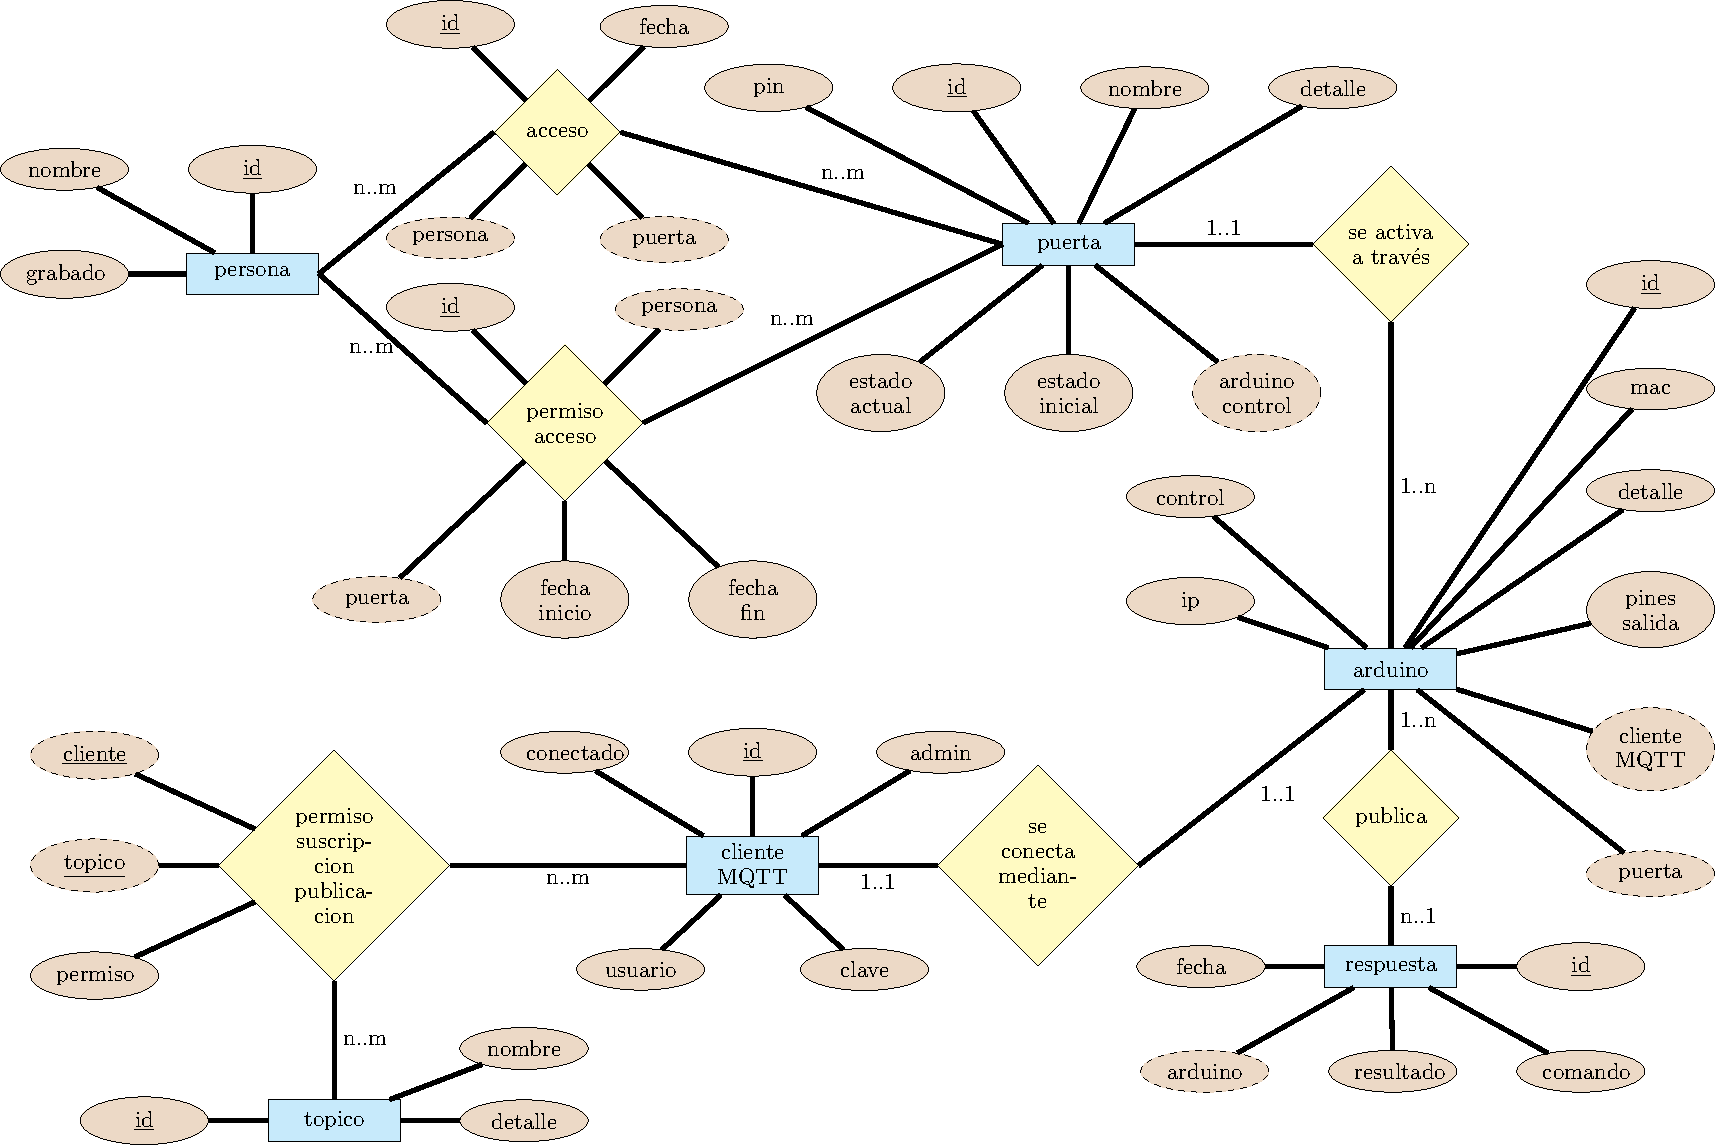
\includegraphics[width=1.3\textwidth]{base_datos_accesos_diagrama.pdf}
      \caption*{\textbf{Fuente:} Elaboración propia}
      \label{fig:base_datos_accesos_diagrama}
    \end{figure}
  \end{landscape}

  Con la reducción de la Tabla \ref{tab:base_datos_accesos_fn3} y la tabla de respuestas de la Tabla \ref{tab:base_datos_accesos_fn2} se consiguió elaborar el diagrama entidad-relación mostrado en la Figura \ref{fig:base_datos_accesos_diagrama}. Mediante el cual se desarrollo la base de datos de la Figura \ref{fig:bd_accesos}.

  Cabe resaltar que el micro-servicio de usuarios se encarga de sincronizar la tabla de \textit{personas} con los datos del servidor LDAP, si se elimina algún usuario del servidor LDAP se eliminan en cascada los datos registrados con el ID del usuario eliminado. Este proceso de sincronización se ejecuta al inicio del sistema y periódicamente de acuerdo al tiempo establecido en las variables de entorno de ejecución, también se puede forzar este proceso mediante un botón en el sistema de administración web que ejecuta la sincronización manual.

  \begin{figure}[H]
    \centering
    \caption{Base de datos de control de accesos}
    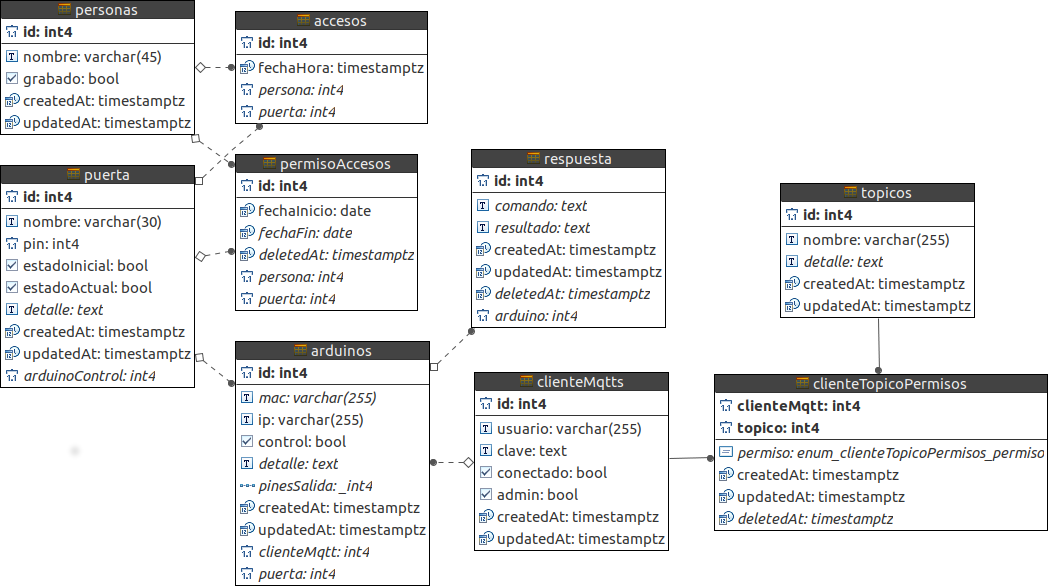
\includegraphics[width=1\textwidth]{ingenieria_proyecto/bd_accesos.png}
    \caption*{\textbf{Fuente:} Elaboración propia}
    \label{fig:bd_accesos}
  \end{figure}

  Esta base de datos está separada de la base de datos de huellas, ya que la base de datos de huellas se puede reutilizar para algún otro sistema que requiera de dichos datos, como por ejemplo un sistema de reloj marcador de hora de ingreso/salida.

  La \textit{lista de usuarios} es una copia exacta de la lista de usuarios de la base de datos de huellas, que a su vez se sincroniza con el servidor de LDAP.

  La siguiente tabla es la de las \textit{puertas}, ésta contiene los datos del nombre código de la puerta, el dispositivo de control y el pin donde se conecta la puerta, el estado lógico inicial y el estado actual que cambia cada vez que la puerta se abre o cierra.

  La tabla de \textit{accesos} es una relación entre el ID de una persona y el ID de una puerta conjuntamente con una fecha y hora en la que se produjo el acceso de una persona.

  Los \textit{permisos de acceso} son una relación entre el ID de una persona y el ID de una puerta donde se diferencian dos tipos de acceso, el indefinido que es un acceso permanente que solo contiene una fecha inicial desde la que la persona podrá acceder por una puerta o el acceso temporal que contiene también una fecha final que es la fecha límite en la cual dicha persona podrá acceder por una puerta.

  La tabla \textit{arduinos} contiene tanto los dispositivos de control, como los dispositivos de interfaz sensorial, la diferencia la define el campo booleano control. Si es un dispositivo de control deberán definirse los pines de salida que estarán disponibles para la tabla \textit{puertas}; mientras que si se trata de un dispositivo de interfaz sensorial debe relacionarse con una puerta ya que controlará el sensor de huellas mediante el cual se abrirá dicha puerta. Ambos tipos de dispositivos deberán relacionarse con un cliente MQTT para conectarse al servidor mediante un usuario y contraseña.
  
  La tabla de \textit{clientes MQTT} contiene el usuario y contraseña para los dispositivos del sistema, así como también contiene un usuario privilegiado que tendrá acceso al sistema servicio web de administración, que además podrá publicar o suscribirse en cualquier tópico del servidor MQTT.

  La tabla \textit{tópicos} contiene todos los tópicos a los cuales los clientes pueden suscribirse o publicar de acuerdo a los permisos definidos en la tabla que relaciona estos permisos.

  Por último la tabla de \textit{respuestas} contiene un historial de todos los comandos del sistema, tanto los que se ejecutan en el servidor como las órdenes hacia los sensores, así como también las respuestas recibidas de cada sensor después de cada orden.

  Cuando se registra un nuevo dispositivo de control se crea automáticamente, el tópico gpio/\textit{:idArduino}/+, donde \textit{idArduino} es reemplazado por el ID del arduino registrado.

  Cuando se registra un dispositivo de interfaz sensorial se crean 3 tópicos automáticamente, c/\textit{:idArduino} que sirve para enviar comandos únicamente a dicho arduino, r/\textit{:idArduino} que sirve para que el arduino publique las respuestas que recibe del sensor de huellas, p/\textit{:idPuerta} que sirve para que el arduino publique el ID de la persona que desea ingresar por dicha puerta. Un tópico adicional es creado cuando se registra el primer dispositivo de interfaz sensorial, c/0 que sirve para enviar comandos a todos los arduinos conectados al sistema.

  \section{Secuencia de acción para la apertura desde el interior}

  \begin{figure}[H]
    \centering
    \caption{Diagrama para la apertura de una puerta desde el interior}
    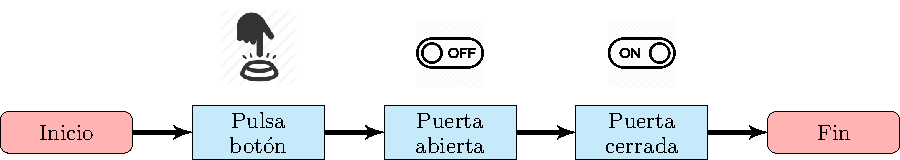
\includegraphics[width=0.95\textwidth]{flujograma_salida.pdf}
    \caption*{\textbf{Fuente:} Elaboración propia}
    \label{fig:flujo_pulsador}
  \end{figure}

  De acuerdo al circuito de la figura \ref{fig:conexion_puerta} y la hoja de datos de la cerradura electromagnética \cite{datasheet:chapa_tesa}, el pin de control de la cerradura vá conectado a un pulsador normalmente abierto con el otro extremo se conecta a tierra; entonces cuando una persona presiona el botón pulsador el pin de control se conecta a tierra haciendo que el pistón de la cerradura se retraiga y la puerta quede abierta por un tiempo, suficiente para que la persona pueda abrir la puerta y salir. Este proceso se realiza enteramente en el lugar donde se halla instalada la cerradura, ya que el pulsador solo necesita conectarse a la misma tierra a la que se conecta la cerradura, por tanto ni el hardware, ni el software desarrollado intervienen en este proceso. Este sistema cuenta con dispositivos que garantizan  una salida libre y sin demora, activada de forma manual\footnote{Portal de salida, Sección 6.1.6, Norma NFPA-731\cite{norma:nfpa_731}}, estos dispositivos de salida requieren una operación de un solo movimiento ininterrumpido\footnote{Dispositivos de salida, Sección 7.2.9, Norma NFPA-730\cite{norma:nfpa_730}}, para que en casos de emergencia las personas que se encuentren dentro de uno de los ambientes que precisen de una salida, acudan a ésta sin ningún tipo de obstrucción, con la respectiva señalización\footnote{Señales de salvamento y evacuación, Norma RM-849-14\cite{norma:rm_849_14}}, ubicada a una altura adecuada\footnote{Ubicación, Sección 2.2, Norma NB-1220004\cite{norma:nb_1220004}} y sin ningún tipo de identificación a fin de poder salir con la mayor facilidad posible para llegar al punto de reunión más cercano.

  \begin{figure}[H]
    \centering
    \caption{Botón pulsador para la apertura desde el interior}
    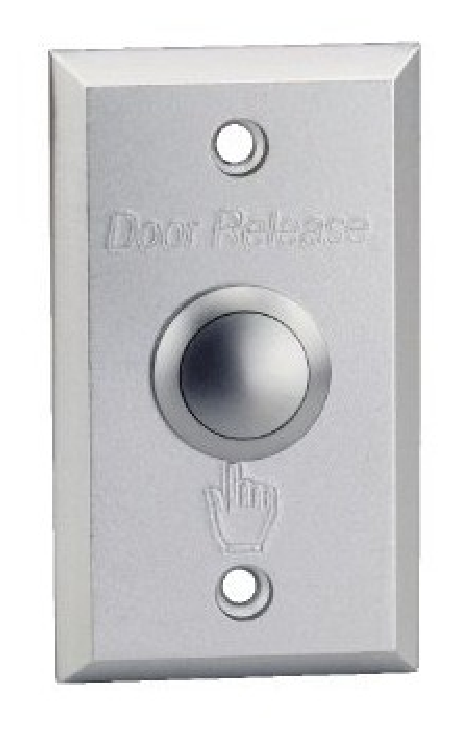
\includegraphics[width=0.1\textwidth]{ingenieria_proyecto/pulsador_pared.eps}
    \caption*{\textbf{Fuente:} \href{https://www.todoelectronica.com/es/pulsador-de-liberacion-de-puerta-salida-de-contacto-no-nc-com-fabricado-en-aluminio-y-acero-p-95904.html}{Pulsador de liberación de puerta, TodoElectrónica.com, España}}
  \end{figure}

  Este dispositivo tiene la además posibilidad de conexión normalmente cerrada, por lo que podría adaptarse a las cerraduras magnéticas de contacto, mismas que no tienen el pin de control, por lo tanto en este caso se debe realizar un ajuste diferente para cortar la alimentación misma; es decir el pin de tierra haría de pin de control e iría conectado al pulsador y desde ahí hasta la placa de control central, logrando de ésta forma un funcionamiento similar al de las cerraduras de pistón.

  \section{Secuencia de acción para el envío de una nueva huella a los sensores}

  \begin{figure}[H]
    \centering
    \caption{Diagrama para envío de huellas a los sensores}
    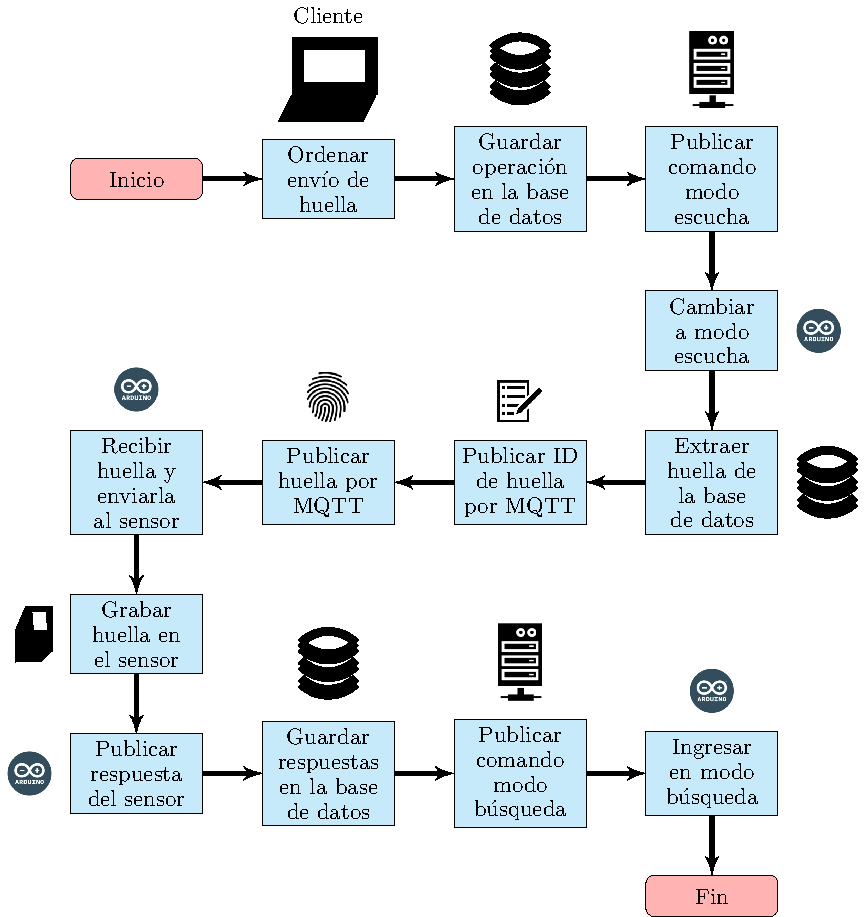
\includegraphics[width=0.95\textwidth]{flujograma_enviar_huella.pdf}
    \caption*{\textbf{Fuente:} Elaboración propia}
    \label{fig:flujo_envio_huella}
  \end{figure}

  Cuando el administrador del sistema inicia el proceso de envío de una huella hacia los sensores, el servidor MQTT publica un comando a los dispositivos de interfaz sensorial:

  \begin{center}
    c/:idDispositivoSensor \quad $ \rightarrow $ \quad :modo
  \end{center}

  El tópico \textit{c} se utiliza para enviar comandos, el ID de dispositivo interfaz sensorial es el que identifica al dispositivo en la base de datos, o de otro modo 0 para enviar comandos a todos los dispositivos y el modo puede ser 0 para cambiar a \textit{modo escucha}, con lo que los dispositivos de interfaz actuarán como un puente entre el servidor y los sensores, en este modo el servidor puede enviar directamente paquetes al lector de huellas, pero con la adición de dos bytes antes de la cabecera de cada paquete de acuerdo al manual del sensor \cite{manual:fingerprint_ZFM-20}. Cuando se envía 1, el modo cambia a \textit{modo búsqueda}, este es el modo predefinido para que los dispositivos busquen una huella en el sensor y envíen el ID de la persona al servidor.

  Por ejemplo el paquete para realizar la operación de handshake en el sensor es el siguiente:

  \begin{table}[H]
    \centering
    \caption{Instrucción de handshake para el sensor de huellas}
    \small
\begin{tabular}{|C{1.6cm}|C{1.6cm}|C{2.1cm}|C{1.6cm}|C{1.6cm}|C{1.6cm}|C{2.1cm}|}
  \hline
  2 bytes & 4 bytes & 1 byte & 2 bytes & 1 byte & 1 byte & 2 bytes \\
  \hline
  Cabecera & Dirección sensor & Indentificador paquete & Tamaño paquete & Código instrucción & Código control & Suma de verificación \\
  \hline
  ef01H & ffffffffH & 01H & 0004H & 17H & 00H & 001cH \\
  \hline
\end{tabular}
    \caption*{\textbf{Fuente:} Manual Sensor ZFM-20, ZhianTec, V1.4, 2008 \cite{manual:fingerprint_ZFM-20}}
  \end{table}

  Para el cual la respuesta del sensor será:

  \begin{table}[H]
    \centering
    \caption{Respuesta de handshake desde el sensor de huellas}
    \small
\begin{tabular}{|C{1.6cm}|C{1.6cm}|C{2.1cm}|C{1.6cm}|C{1.6cm}|C{2.1cm}|}
  \hline
  2 bytes & 4 bytes & 1 byte & 2 bytes & 1 byte & 2 bytes \\
  \hline
  Cabecera & Dirección sensor & Indentificador paquete & Tamaño paquete & Código instrucción & Suma de verificación \\
  \hline
  ef01H & ffffffffH & 07H & 0003H & xxH & sumH \\
  \hline
\end{tabular}
    \caption*{\textbf{Fuente:} Manual Sensor ZFM-20, ZhianTec, V1.4, 2008 \cite{manual:fingerprint_ZFM-20}}
  \end{table}

  Mediante este comportamiento se puede observar que el tamaño total del paquete de respuesta del sensor es de 12 bytes (0cH) y que además el byte de respuesta se encuentra en la posición 9 (09H), con estos datos se desarrolló una librería para comunicarse con el sensor mediante el hardware de interfaz sensorial en \textit{modo 0}.

  \begin{table}[H]
    \centering
    \caption{Instrucción modificada de handshake para el sensor de huellas}
    \tiny
\begin{tabular}{|C{1.2cm}|C{1.4cm}|C{1.2cm}|C{1.2cm}|C{1.4cm}|C{1.2cm}|C{1.2cm}|C{1.2cm}|C{1.4cm}|}
  \hline
  1 byte & 1 byte & 2 bytes & 4 bytes & 1 byte & 2 bytes & 1 byte & 1 byte & 2 bytes \\
  \hline
  Tamaño respuesta & Posición byte respuesta & Cabecera & Dirección sensor & Indentificador paquete & Tamaño paquete & Código instrucción & Código control & Suma de verificación \\
  \hline
  0cH & 09H & ef01H & ffffffffH & 01H & 0004H & 17H & 00H & 001cH \\
  \hline
\end{tabular}
    \caption*{\textbf{Fuente:} Elaboración propia}
  \end{table}

  Donde el primer byte indica el tamaño de paquete de respuesta que debe esperar el dispositivo de interfaz sensorial y el siguiente byte indica la posición de donde se extraerá la respuesta para enviarla al servidor.

  Entonces con este protocolo modificado el servidor publicará hacia el dispositivo cuya ID es igual a 1:

  \begin{center}
    c/1 \quad $ \rightarrow $ \quad 0c09ef01ffffffff0100041700001c
  \end{center}

  El dispositivo de interfaz sensorial 1 recibirá este paquete, extraerá los 2 primeros bytes para su uso y reenviará lo demás hacia el sensor de huellas. El sensor de huellas responderá de acuerdo a su estado y el dispositivo de interfaz sensorial publicará la respuesta recibida desde el sensor.

  \begin{center}
    r/1 \quad $ \rightarrow $ \quad 00
  \end{center}

  En caso de que el sensor se encuentre conectado y se halle funcionando este valor \textit{00} indica que el ``Proceso se realizó con éxito``. Esta respuesta literal será la que se envíe hasta el servicio web para obtener en tiempo real todas las respuestas de los sensores conectados al sistema.

  De este mismo modo es como se enviarán las huellas almacenadas en la base de datos hacia los sensores mediante la librería desarrollada para los sensores de huella dactilar ZFM-20.

  Después de enviar todas las huellas a los sensores el servidor vuelve a poner los mismos en \textit{modo búsqueda}. Cabe resaltar que durante el proceso de comunicación servidor-sensores, el sistema entrará en un estado de ``Ocupado`` en el cual no recibirá más órdenes hasta terminar todo el proceso.

  \section{Secuencia de acción para la apertura mediante el respaldo bluetooth}

  Se ha desarrollado un circuito bluetooth con el microcontrolador ATtiny85 y el módulo bluetooth HC-06, en base al esquema de \href{http://arduino-projects4u.com/attiny85-arduino/}{attiny85 arduino de www.arduino-projects4u.com}. Se puede observar el esquema de este dispositivo en el Anexo \ref{anx:esquema_respaldo_bluetooth}.

  En caso de que el servidor MQTT dejase de operar y fuera necesario el acceso físico hasta el servidor, este dispositivo se puede instalar en una de las puertas menos críticas para poder realizar los arreglos necesarios para volver a levantar el sistema. Este dispositivo deberá ser operado solo por una persona con un nivel mas alto que el administrador y deberá tener conocimientos del sistema para realizar el mantenimiento del mismo.

  \begin{figure}[h]
    \centering
    \caption{Diagrama para apertura mediante respaldo bluetooth}
    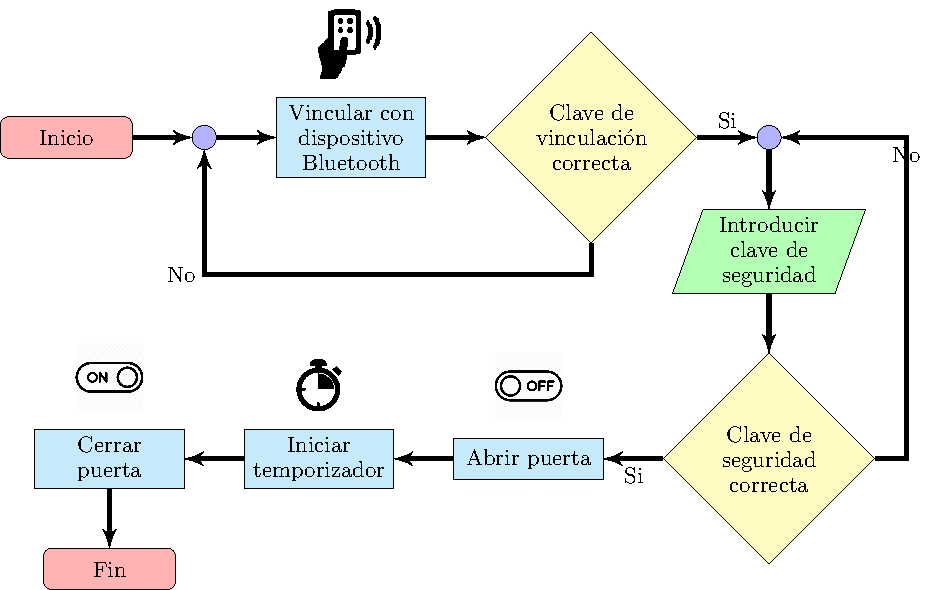
\includegraphics[width=0.94\textwidth]{flujograma_bluetooth.pdf}
    \caption*{\textbf{Fuente:} Elaboración propia}
    \label{fig:flujo_respaldo_bluetooth}
  \end{figure}

  Este dispositivo tiene dos pasos de seguridad, el primero es una contraseña definida en el módulo HC-06 para la vinculación de un bluetooth en modo esclavo, el segundo paso es el envío de una contraseña mediante una aplicación Android para abrir una de las dos puertas que puede controlar el dispositivo.

  \begin{figure}[H]
    \centering
    \caption{Pantalla de vinculación de la aplicación Android}
    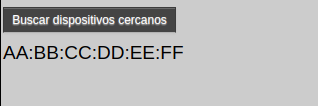
\includegraphics[width=0.45\textwidth]{ingenieria_proyecto/android_pantalla_1.png}
    \caption*{\textbf{Fuente:} Elaboración propia}
    \label{fig:android_pantalla_1}
  \end{figure}

  Como medida de seguridad contra ataques de fuerza bruta, el dispositivo bluetooth tiene una restricción en el número de intentos que se puede realizar antes de entrar en un modo de reposo durante un tiempo definido. Por defecto se pedirá la contraseña tres veces, en caso de fallar todos los intentos el dispositivo no se encontrará disponible hasta dentro de 30 minutos. También hay un tiempo de espera entre cada intento que por defecto es de 3 segundos, antes de este tiempo no se podrá realizar otro intento de apertura. Estas variables se pueden cambiar al momento de la programación del microcontrolador.

  \begin{figure}[H]
    \centering
    \caption{Pantalla de envío de contraseña de la aplicación Android}
    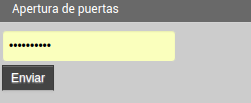
\includegraphics[width=0.45\textwidth]{ingenieria_proyecto/android_pantalla_2.png}
    \caption*{\textbf{Fuente:} Elaboración propia}
    \label{fig:android_pantalla_2}
  \end{figure}

  Este dispositivo debe instalarse a menos de 10 metros de la puerta de ingreso para obtener una conexión fiable y evitar atenuación o interferencias en la comunicación al momento de enviar la contraseña de apertura.

  La idea de este dispositivo fué adaptada del artículo ``Encender un Led con Android y Arduino vía Bluetooth'', ElectronicaStore.Net, 15 de Marzo de 2016 \cite{web:nano_hc_05}.

  \begin{figure}[H]
    \centering
    \caption{Conexión del módulo bluetooth HC-05}
    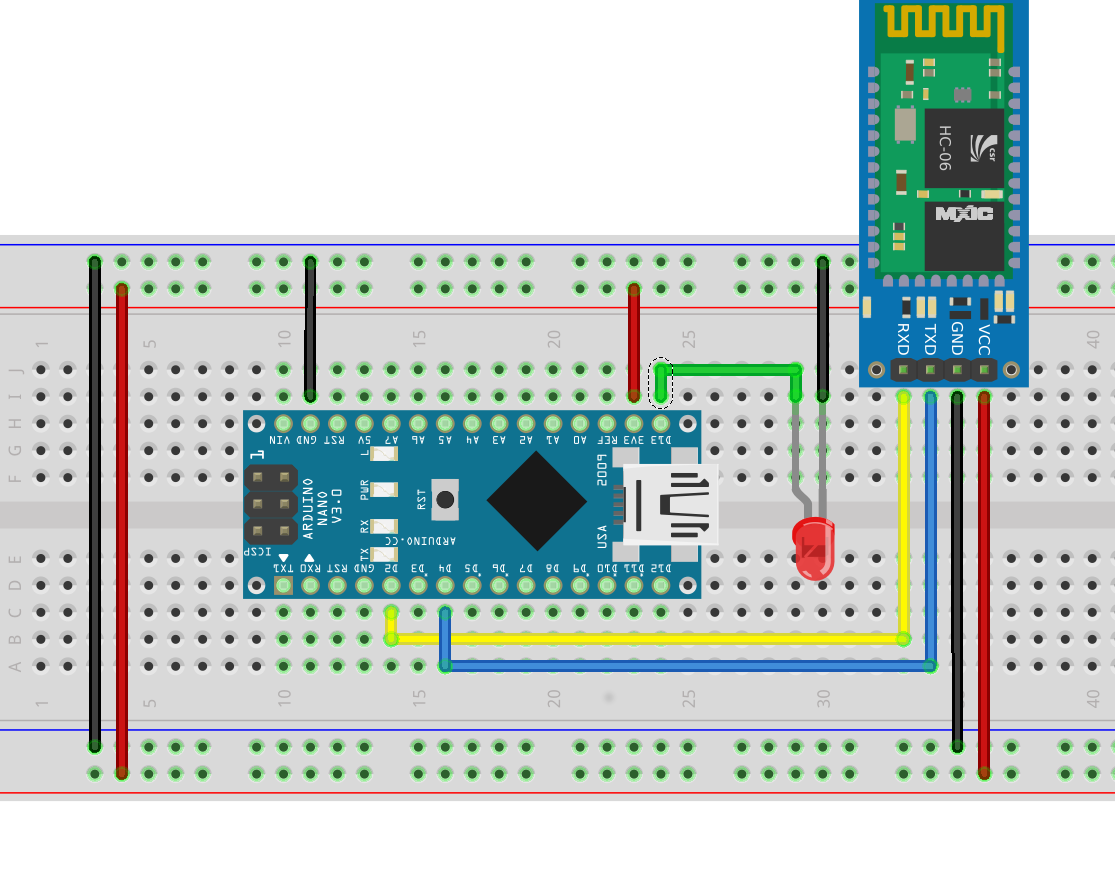
\includegraphics[width=0.65\textwidth]{ingenieria_proyecto/nano_hc_05.png}
    \caption*{\textbf{Fuente:} Encender un Led con Android y Arduino vía Bluetooth, ElectronicaStore.Net, 15 de Marzo de 2016 \cite{web:nano_hc_05}.}
  \end{figure}

  \section{Servicio web para la administración del sistema}

  Como se puede observar en la base de datos de la figura \ref{fig:bd_accesos} existe un campo nombrado \textit{admin}, los clientes que tengan habilitado este campo tendrán acceso al sistema web de administración.

  \begin{figure}[H]
    \centering
    \caption{Página de login del servicio web}
    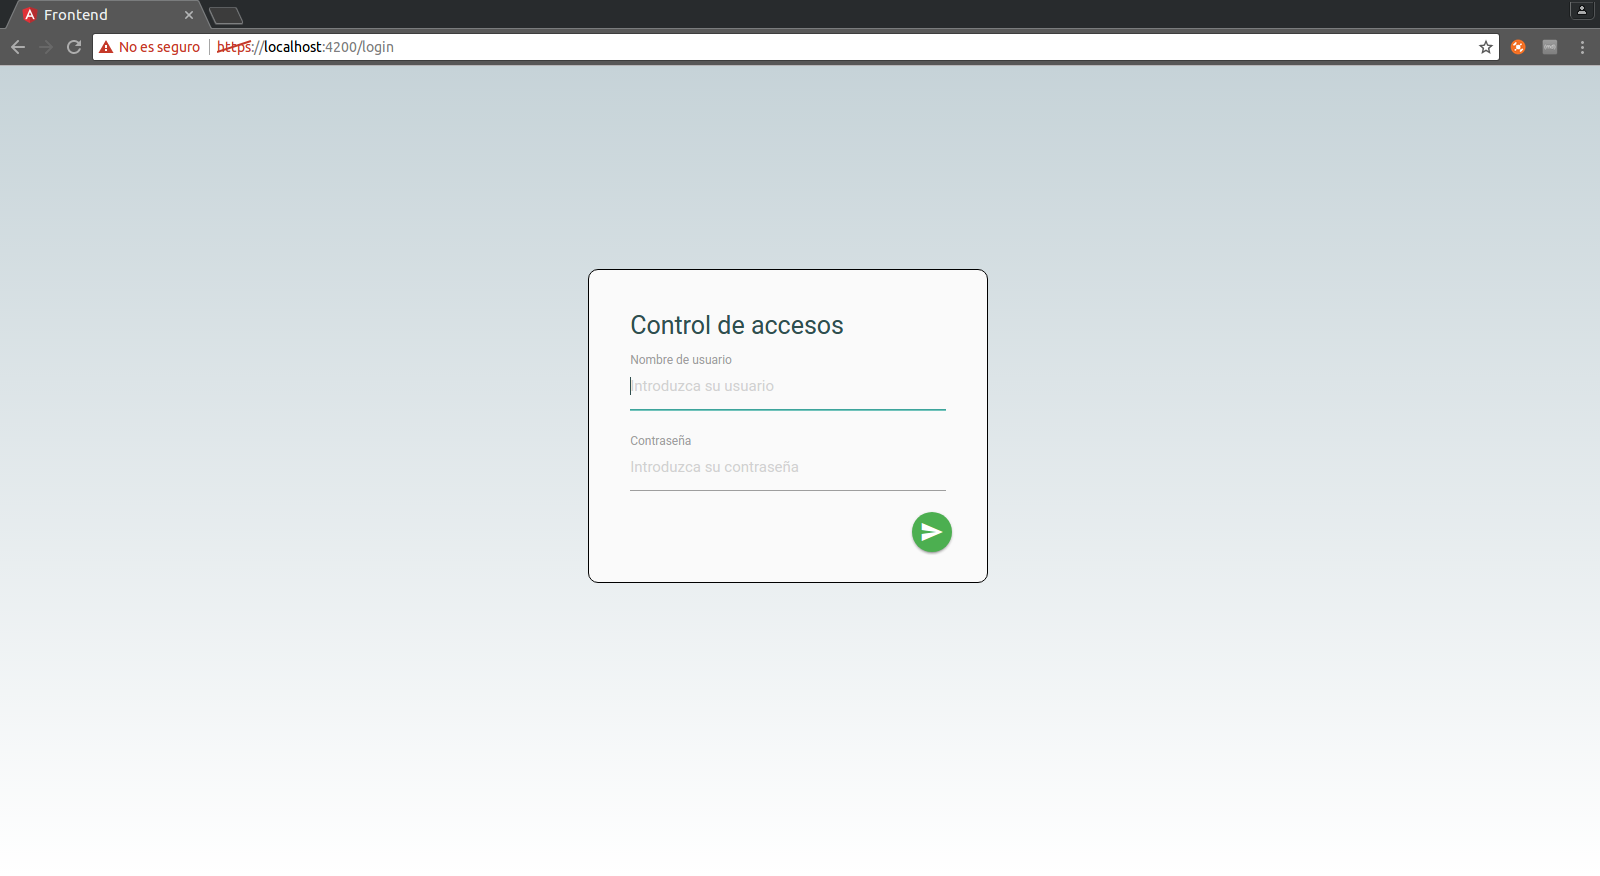
\includegraphics[width=0.95\textwidth]{ingenieria_proyecto/web_login.png}
    \caption*{\textbf{Fuente:} Elaboración propia}
    \label{fig:web_login}
  \end{figure}

  Una vez que se ingresa al sistema se observa una página con el estado de las puertas y un resumen de los últimos accesos ordenados por fecha de manera descendente, el estado de las puertas se identifica por un color rojo cuando se encuentran abiertas, además de un ícono con forma de candado abierto; cuando las puertas se cierran cambian a un color verde con el ícono de un candado cerrado. Tanto estos estados como la lista de últimos accesos cambia de forma dinámica en tiempo real para poder realizar el monitoreo por ejemplo desde una sala de seguridad o de control.

  \begin{figure}[H]
    \centering
    \caption{Página de monitoreo del servicio web}
    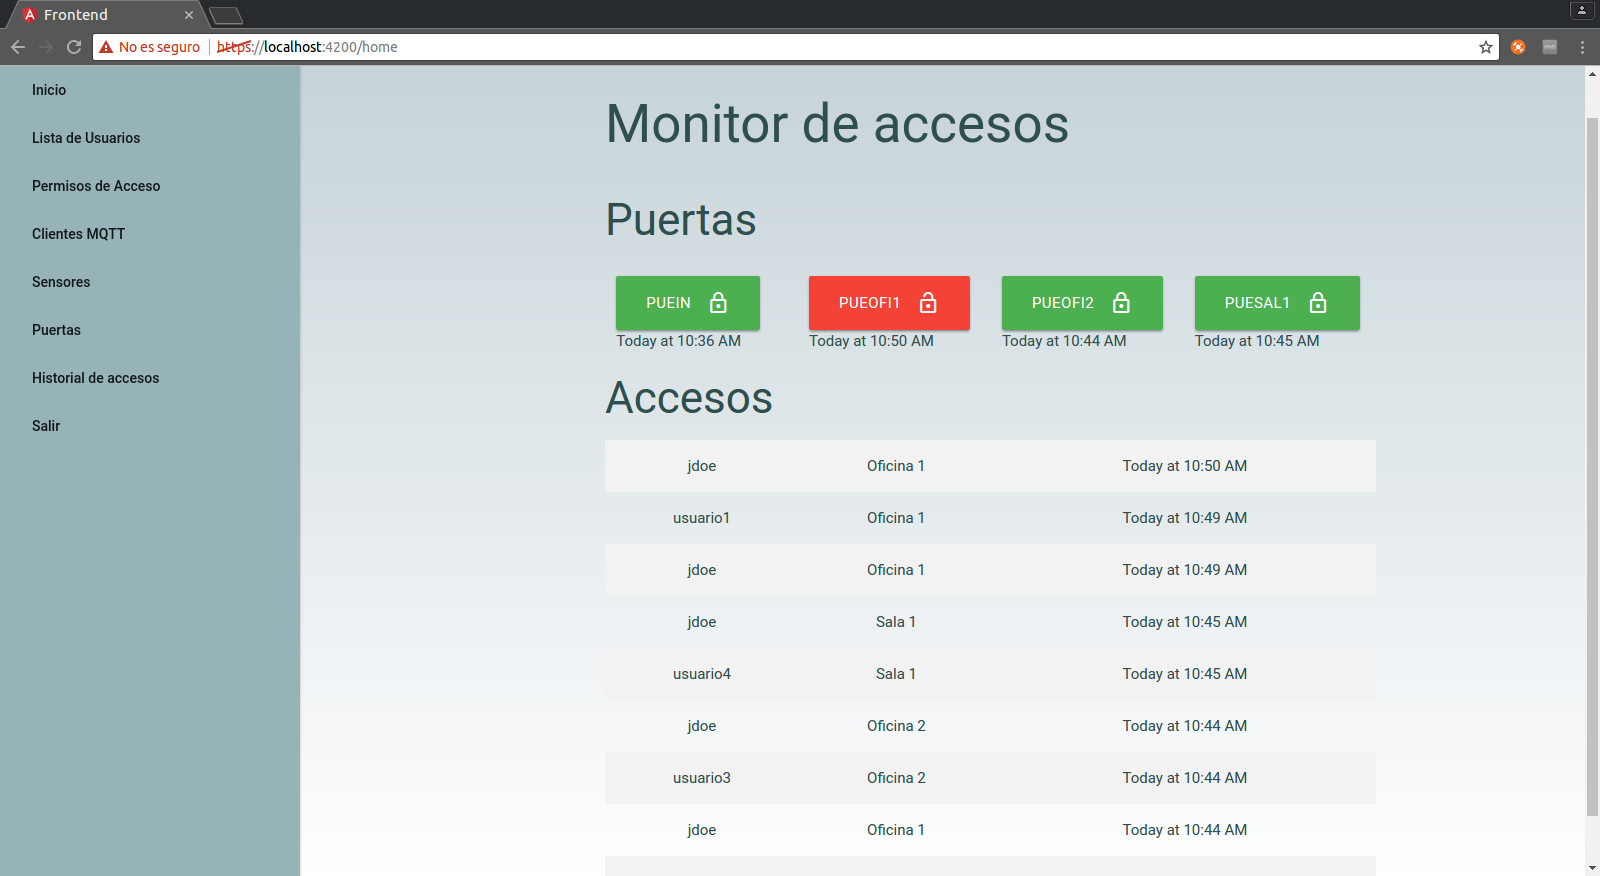
\includegraphics[width=0.95\textwidth]{ingenieria_proyecto/web_monitor.png}
    \caption*{\textbf{Fuente:} Elaboración propia}
    \label{fig:web_monitor}
  \end{figure}

  Al extremo izquierdo se puede navegar por las diferentes páginas para administrar el sistema, la primera página es la lista de usuarios, en esta tenemos un botón en la parte superior \textbf{FORZAR SINCRONIZACIÓN} que actualiza la lista de usuarios sincronizando los valores con los almacenados en el servidor LDAP. Debajo está la tabla donde se halla el primer botón que sirve para grabar o actualizar las huellas de los usuarios, el segundo botón es el de enviar huella, este cambia de color naranja a verde cuando se ha realizado el envío de dicha huella a los sensores conectados al sistema, por último está el botón borrar huella que borra la huella elegida de los sensores. Cuando se pulsa \textbf{Grabar huella} y el proceso no se completa, o se presiona el botón \textbf{Borrar huella}, el color de \textbf{Enviar huella} cambia de verde a naranja.

  \begin{figure}[H]
    \centering
    \caption{Página de lista de usuarios del servicio web}
    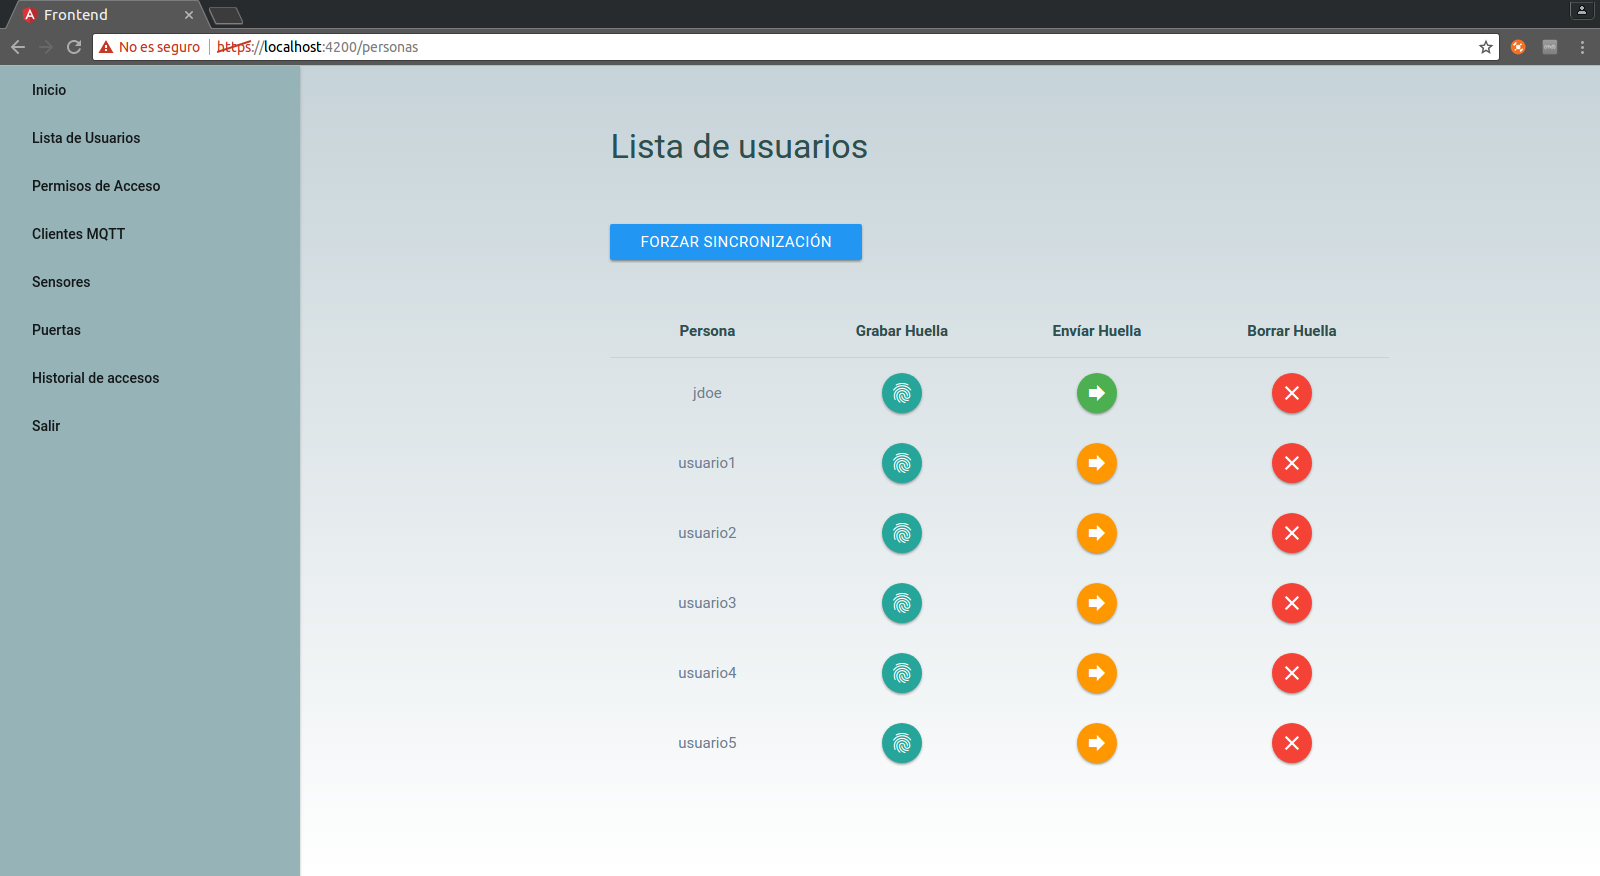
\includegraphics[width=0.95\textwidth]{ingenieria_proyecto/web_lista_usuarios.png}
    \caption*{\textbf{Fuente:} Elaboración propia}
    \label{fig:web_lista_usuarios}
  \end{figure}

  Si se hace clic sobre algún nombre de usuario de la tabla de la figura \ref{fig:web_lista_usuarios} se muestra la imagen de la huella del usuario seleccionado.

  \begin{figure}[H]
    \centering
    \caption{Página de imagen de la huella del servicio web}
    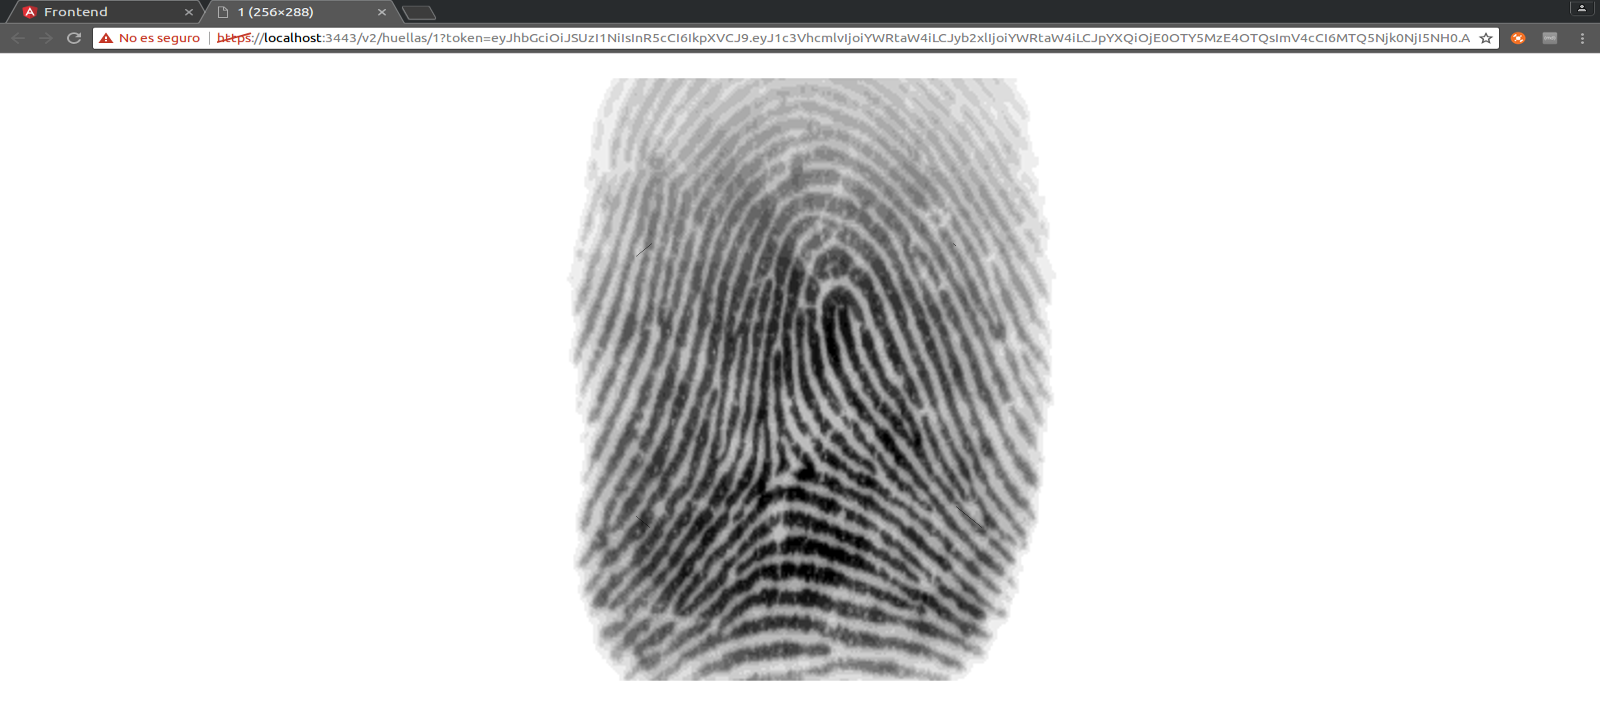
\includegraphics[width=0.95\textwidth]{ingenieria_proyecto/web_imagen_huella.png}
    \caption*{\textbf{Fuente:} Elaboración propia}
    \label{fig:web_imagen_huella}
  \end{figure}

  La página de permisos de acceso contiene dos vistas, la de permisos indefinidos, es decir aquellos que no tienen una fecha final y que estarán habilitados hasta que se los deshabilite. En esta página se ve la lista de usuarios y las puertas por las cuales tiene acceso cada uno; en la primera fila de la tabla se pueden añadir nuevos accesos eligiendo un usuario que no se encuentre en la lista de abajo y haciendo clic en la puerta a la que se le desea dar acceso.

  \begin{figure}[H]
    \centering
    \caption{Página de permisos indefinidos del servicio web}
    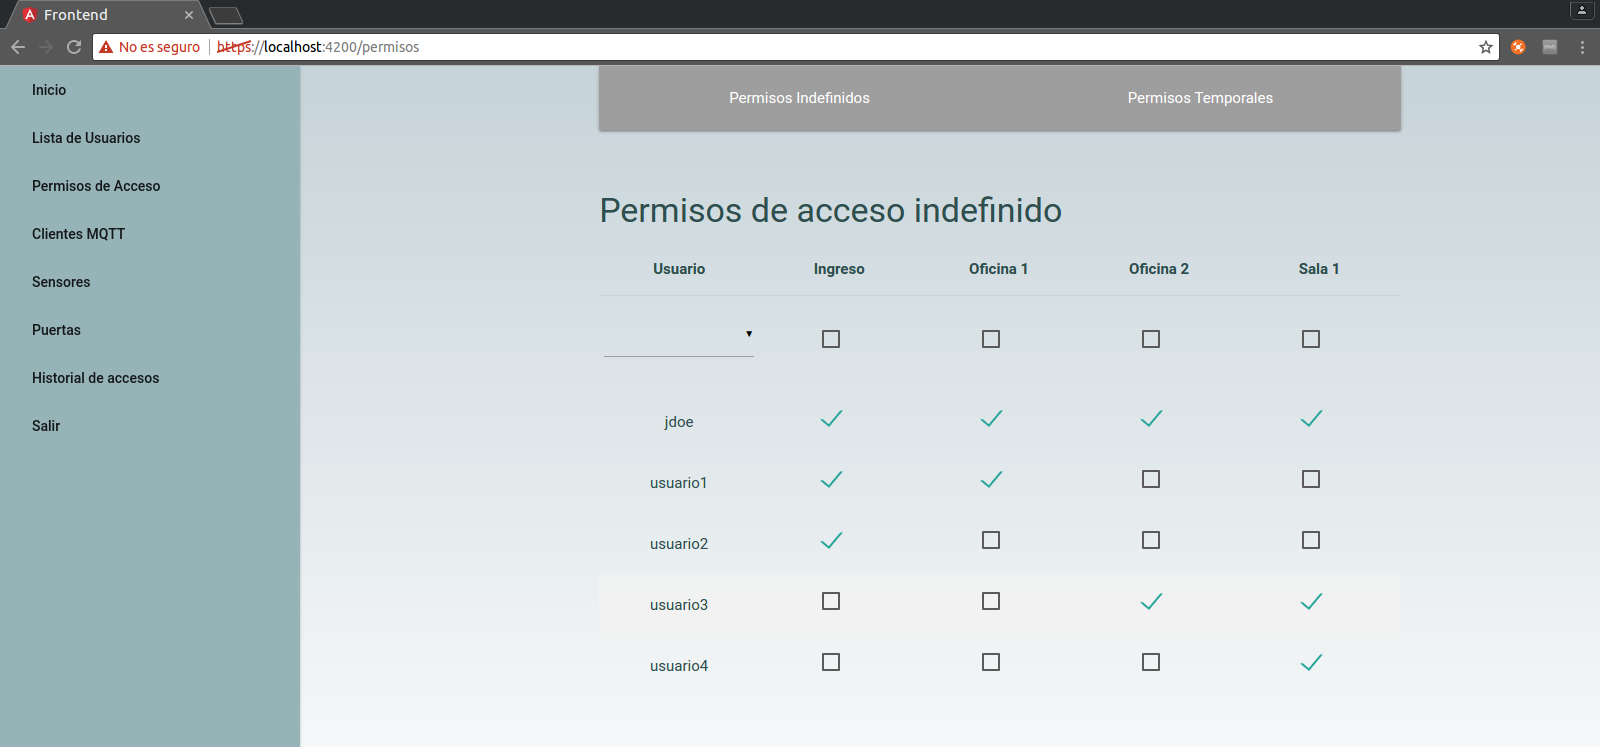
\includegraphics[width=0.95\textwidth]{ingenieria_proyecto/web_permisos_indefinidos.png}
    \caption*{\textbf{Fuente:} Elaboración propia}
    \label{fig:web_permisos_indefinidos}
  \end{figure}

  La otra vista es la de permisos temporales, son aquellos que tienen una fecha final en la cual el usuario podrá acceder por dicha puerta, en la primera fila se pueden crear nuevos permisos temporales eligiendo un usuario y una puerta, una fecha de inicio y una fecha final del permiso concedido, ambos son inclusivos, es decir que el usuario elegido podrá acceder desde las 00:00 horas de la fecha inicial hasta las 24:00 horas de la fecha final. En la tabla de abajo se tienen los permisos activos, estos se pueden modificar en ambas fechas y también se pueden eliminar con el botón \textbf{X}.

  \begin{figure}[H]
    \centering
    \caption{Página de permisos temporales del servicio web}
    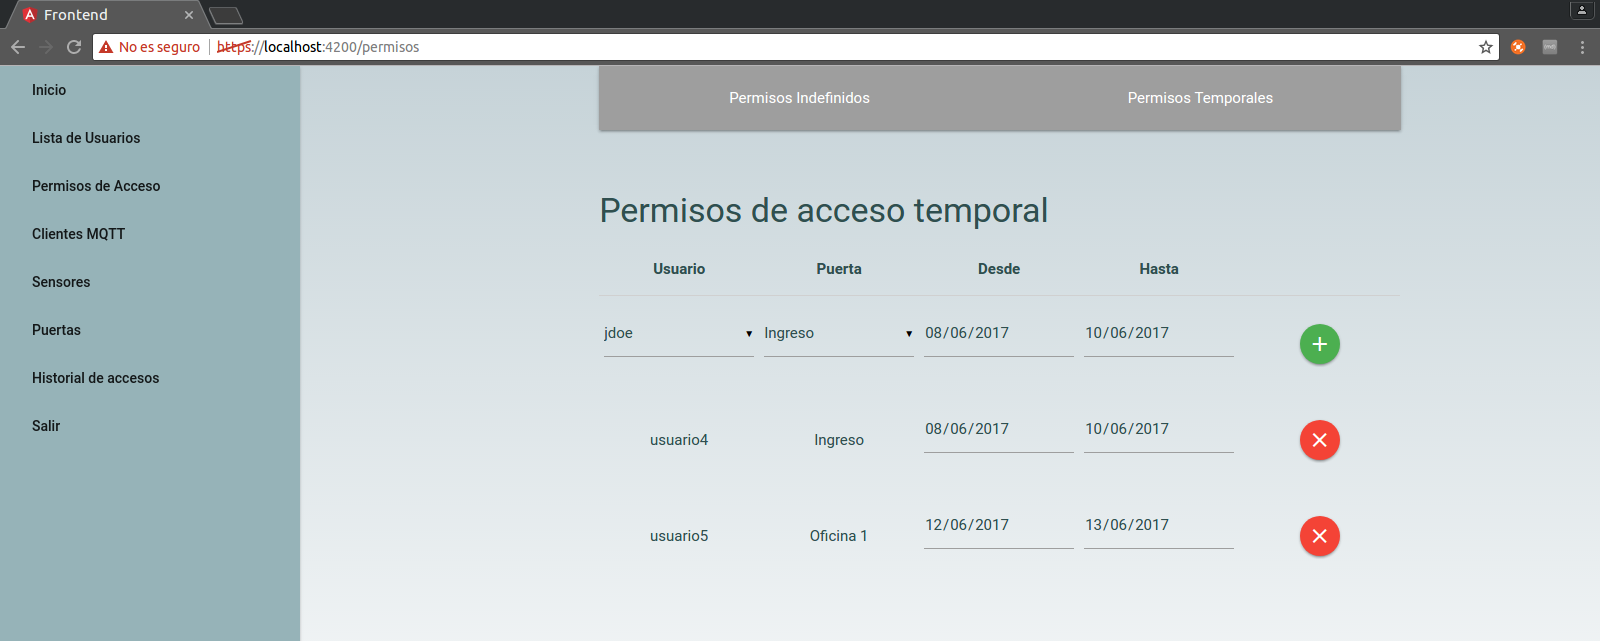
\includegraphics[width=0.95\textwidth]{ingenieria_proyecto/web_permisos_temporales.png}
    \caption*{\textbf{Fuente:} Elaboración propia}
    \label{fig:web_permisos_temporales}
  \end{figure}

  La página de clientes MQTT alberga todos los clientes con los que los dispositivos de hardware se conectan al sistema, también tienen los clientes administradores que pueden suscribirse o publicar en cualquier tópico del servidor MQTT e ingresar al sistema web. Cabe resaltar que un usuario no puede conectarse múltiples veces al sistema, por lo cual si se desea tener un monitor del sistema por ejemplo en una televisión en un ambiente de seguridad como se realiza típicamente se deberá crear un usuario administrador diferente al usuario que se utiliza para realizar cambios, brindar permisos, etc.

  Por otra parte cada usuario solo puede estar conectado en una instancia, lo cual brinda una capa más de seguridad al sistema ya que no se puede suplantar la identidad de un dispositivo si este ya se encuentra conectado.

  \begin{figure}[H]
    \centering
    \caption{Página de clientes MQTT del servicio web}
    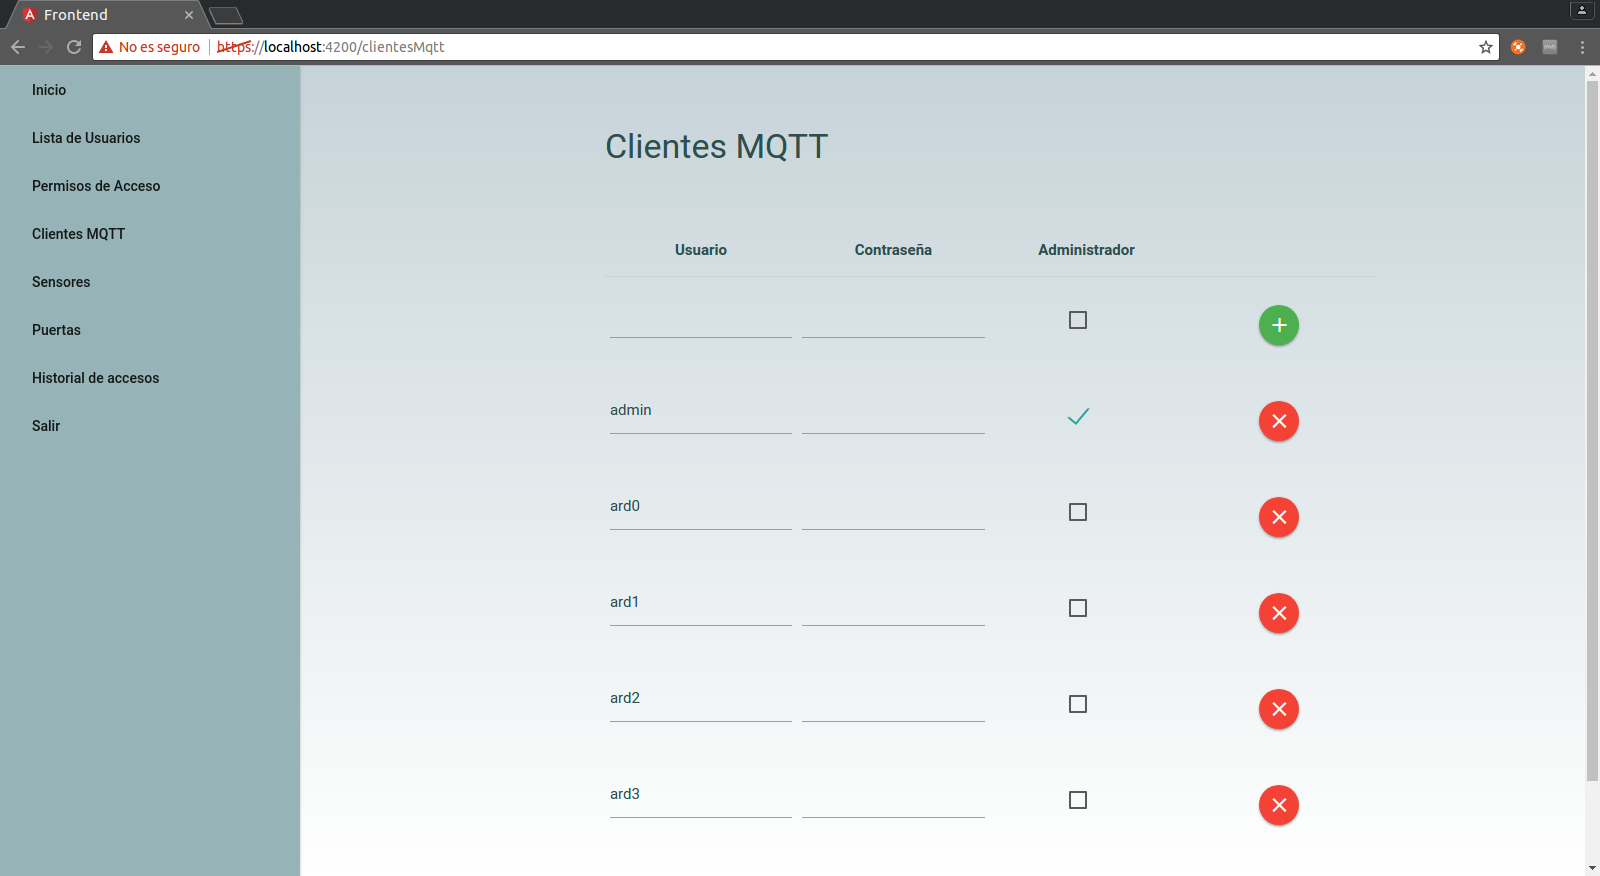
\includegraphics[width=0.95\textwidth]{ingenieria_proyecto/web_clientes_mqtt.png}
    \caption*{\textbf{Fuente:} Elaboración propia}
    \label{fig:web_clientes_mqtt}
  \end{figure}

  La página de sensores tiene dos vistas, la primera es la de dispositivos de control, en esta se le asigna un nombre a cada dispositivo, la dirección IP, la dirección MAC, los pines de salida en caso de utilizar otro microcontrolador o utilizar más pines del mismo ATmega328P, por último se asigna un cliente MQTT a cada dispositivo para que pueda conectarse al sistema.

  Una vez creado un dispositivo éste se mueve a la tabla inferior, donde se pueden actualizar sus datos, tomando en cuenta que la dirección IP y la dirección MAC deberán ser únicas; es decir, no se deben repetir, al igual que el cliente MQTT.

  El sistema no permitirá la creación de un nuevo dispositivo si no se encuentra ningún cliente MQTT registrado.

  \begin{figure}[H]
    \centering
    \caption{Página de dispositivos de control del servicio web}
    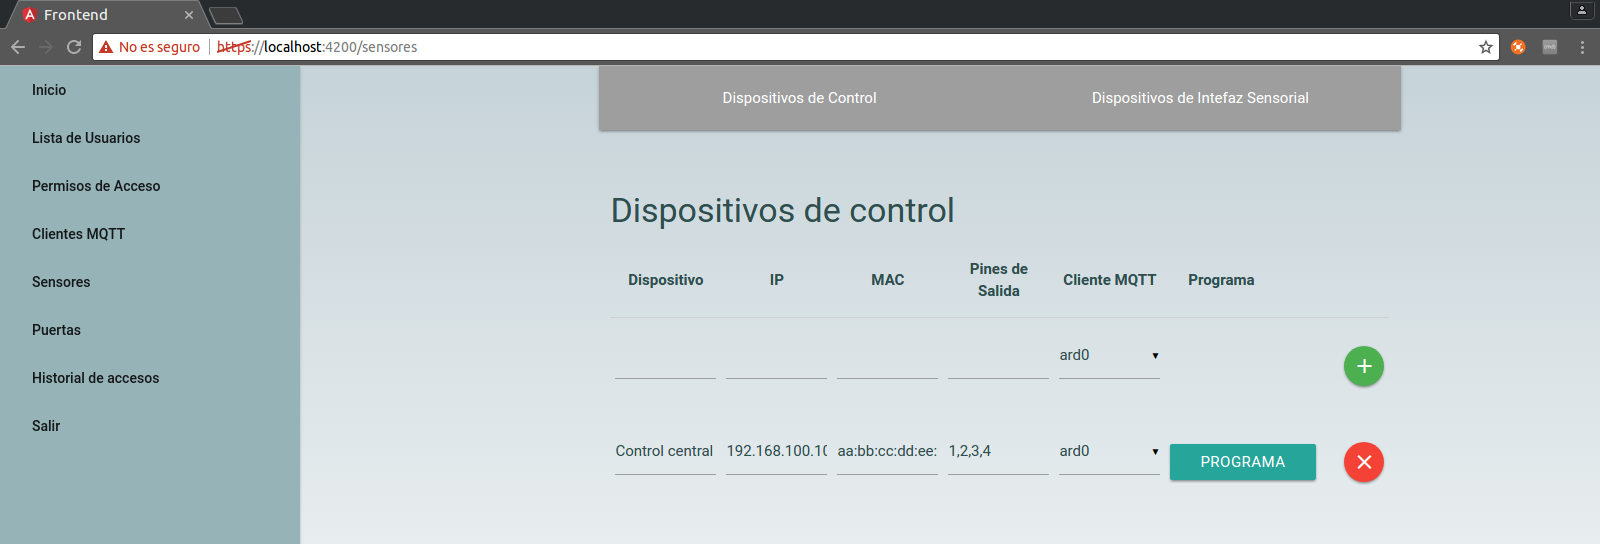
\includegraphics[width=0.95\textwidth]{ingenieria_proyecto/web_controladores.png}
    \caption*{\textbf{Fuente:} Elaboración propia}
    \label{fig:web_controladores}
  \end{figure}

  En la vista que se muestra en la figura \ref{fig:web_controladores} se encuentra el botón \textbf{PROGRAMA} que al pulsarlo nos devuelve el código listo para grabar en el dispositivo de control mediante el software \href{https://www.arduino.cc/en/main/software}{Arduino IDE}, mismo que ya debe tener instaladas todas las librerías necesarias para grabar los dispositivos.

  \begin{figure}[H]
    \centering
    \caption{Página de programa de control del servicio web}
    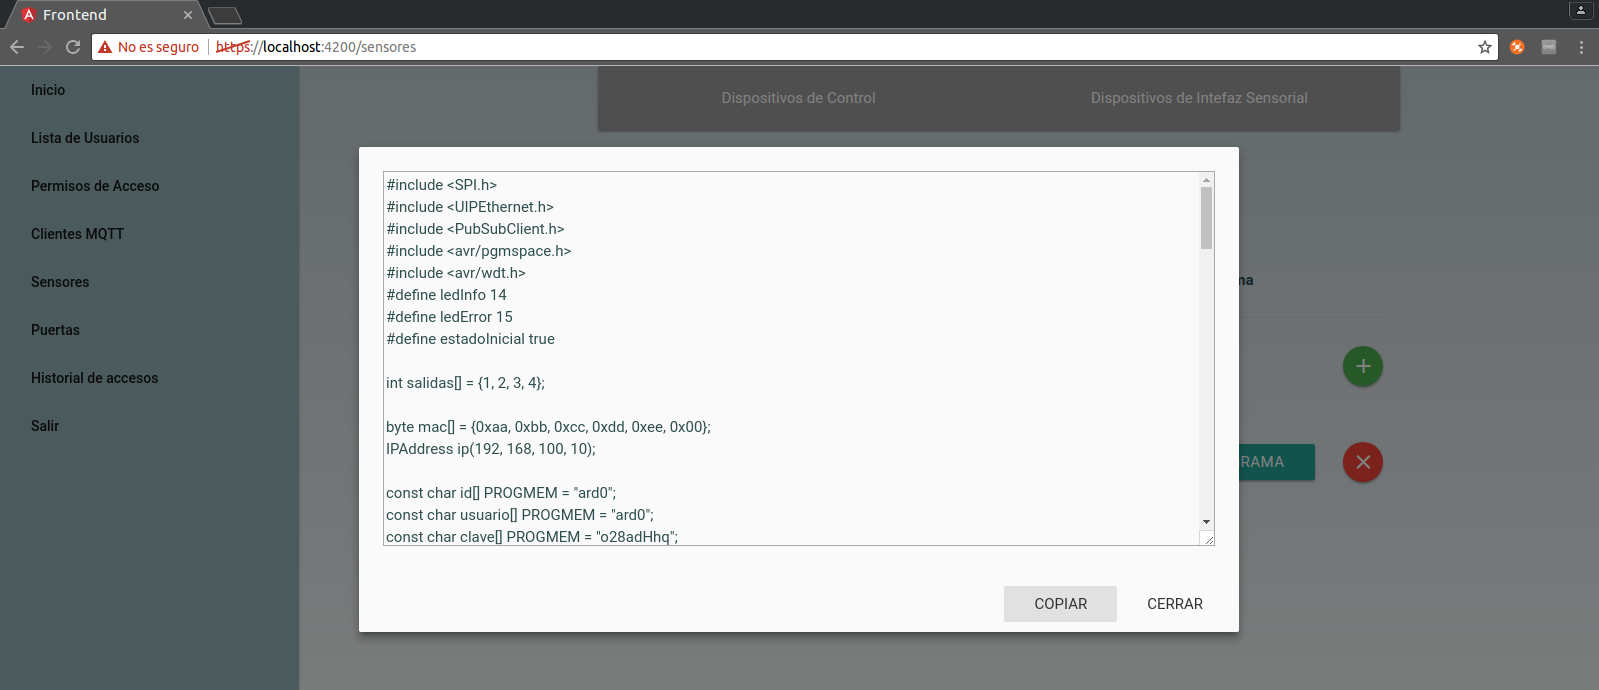
\includegraphics[width=0.95\textwidth]{ingenieria_proyecto/web_programa_control.png}
    \caption*{\textbf{Fuente:} Elaboración propia}
    \label{fig:web_programa_control}
  \end{figure}

  La vista de la página de dispositivos de interfaz sensorial tiene una lógica parecida, pero en lugar de los pines de salida el dispositivo se relaciona con una de las puertas registradas.

  \begin{figure}[H]
    \centering
    \caption{Página de dispositivos de interfaz sensorial del servicio web}
    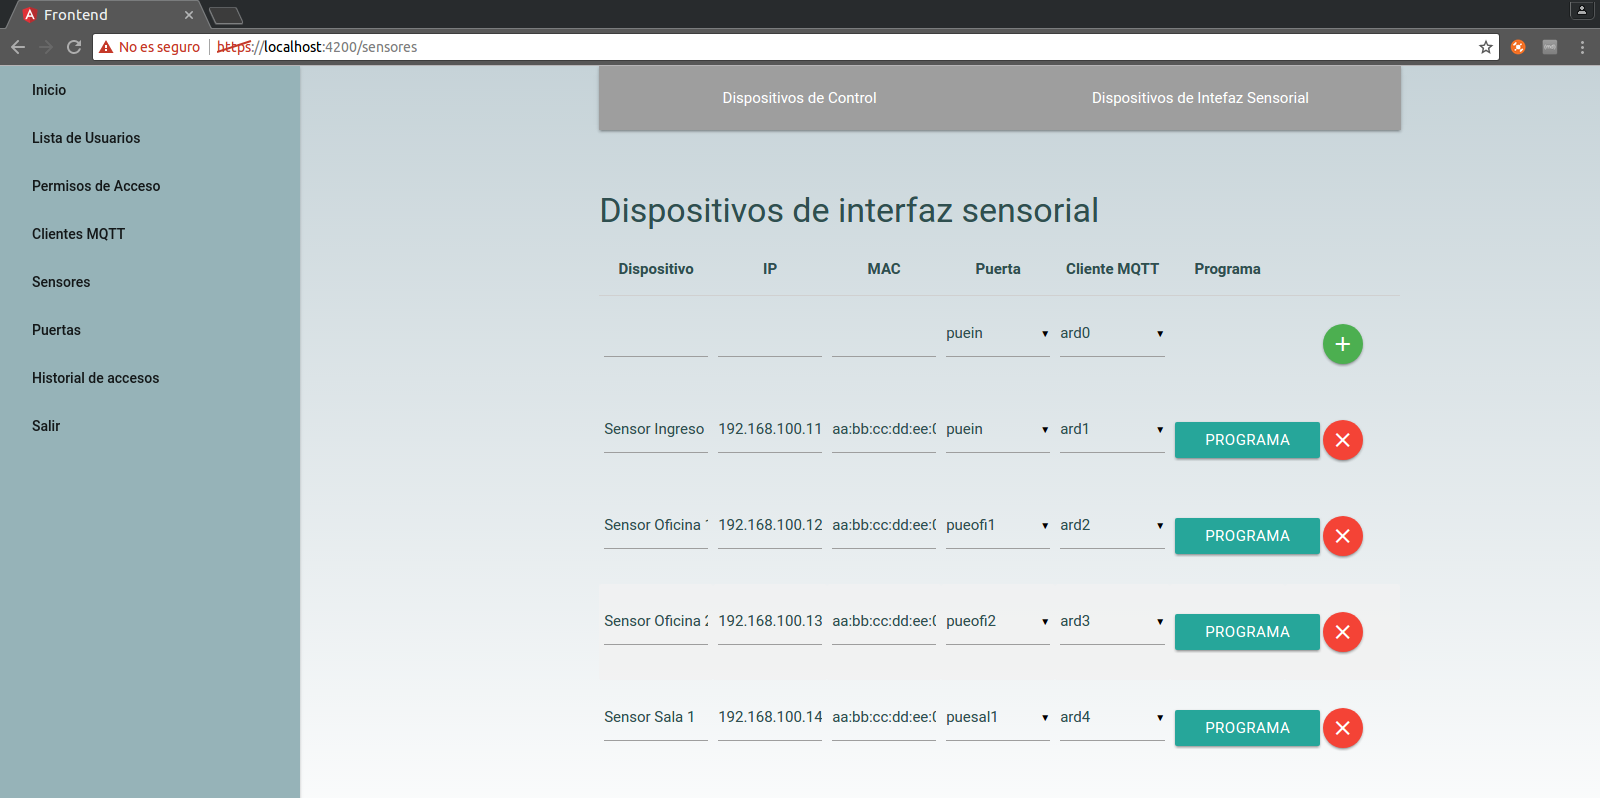
\includegraphics[width=0.95\textwidth]{ingenieria_proyecto/web_sensores.png}
    \caption*{\textbf{Fuente:} Elaboración propia}
    \label{fig:web_sensores}
  \end{figure}

  De igual forma al pulsar el botón \textbf{PROGRAMA} nos devuelve el código listo para grabar en el dispositivo de interfaz sensorial.

  \begin{figure}[H]
    \centering
    \caption{Página de programa de interfaz sensorial del servicio web}
    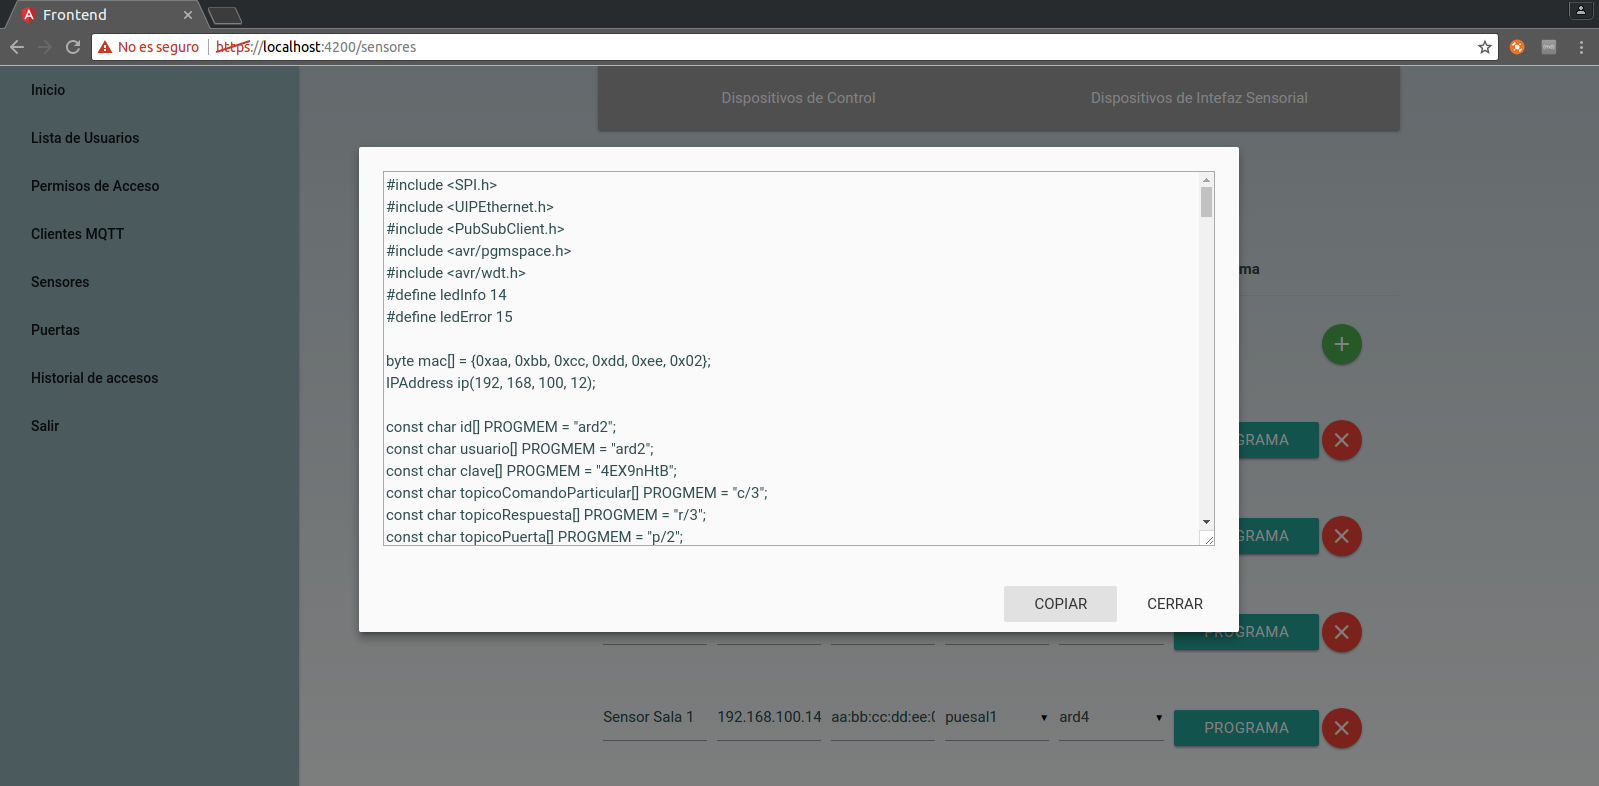
\includegraphics[width=0.95\textwidth]{ingenieria_proyecto/web_programa_sensor.png}
    \caption*{\textbf{Fuente:} Elaboración propia}
    \label{fig:web_programa_sensor}
  \end{figure}

  La página de puertas tiene los siguientes campos: un código único que identifica cada puerta, el detalle que es un nombre mas legible para las personas, el estado inicial de la lógica de la puerta; es decir, si la puerta debe iniciar cerrada con un nivel alto en el pin de control este valor tendrá que ser establecido en nivel alto también.

  El hardware de control es el dispositivo que controla la puerta, el sistema se ha dimensionado para que cada dispositivo de control pueda abrir o cerrar hasta seis puertas, esto debido a los pines disponibles en el microcontrolador.

  Por último se define en cual de los pines del dispositivo de control irá conectado el pin de control de la puerta, este valor también es único ya que una sola puerta podrá ir conectada a cada pin definido en el hardware de control.

  \begin{figure}[H]
    \centering
    \caption{Página de puertas del servicio web}
    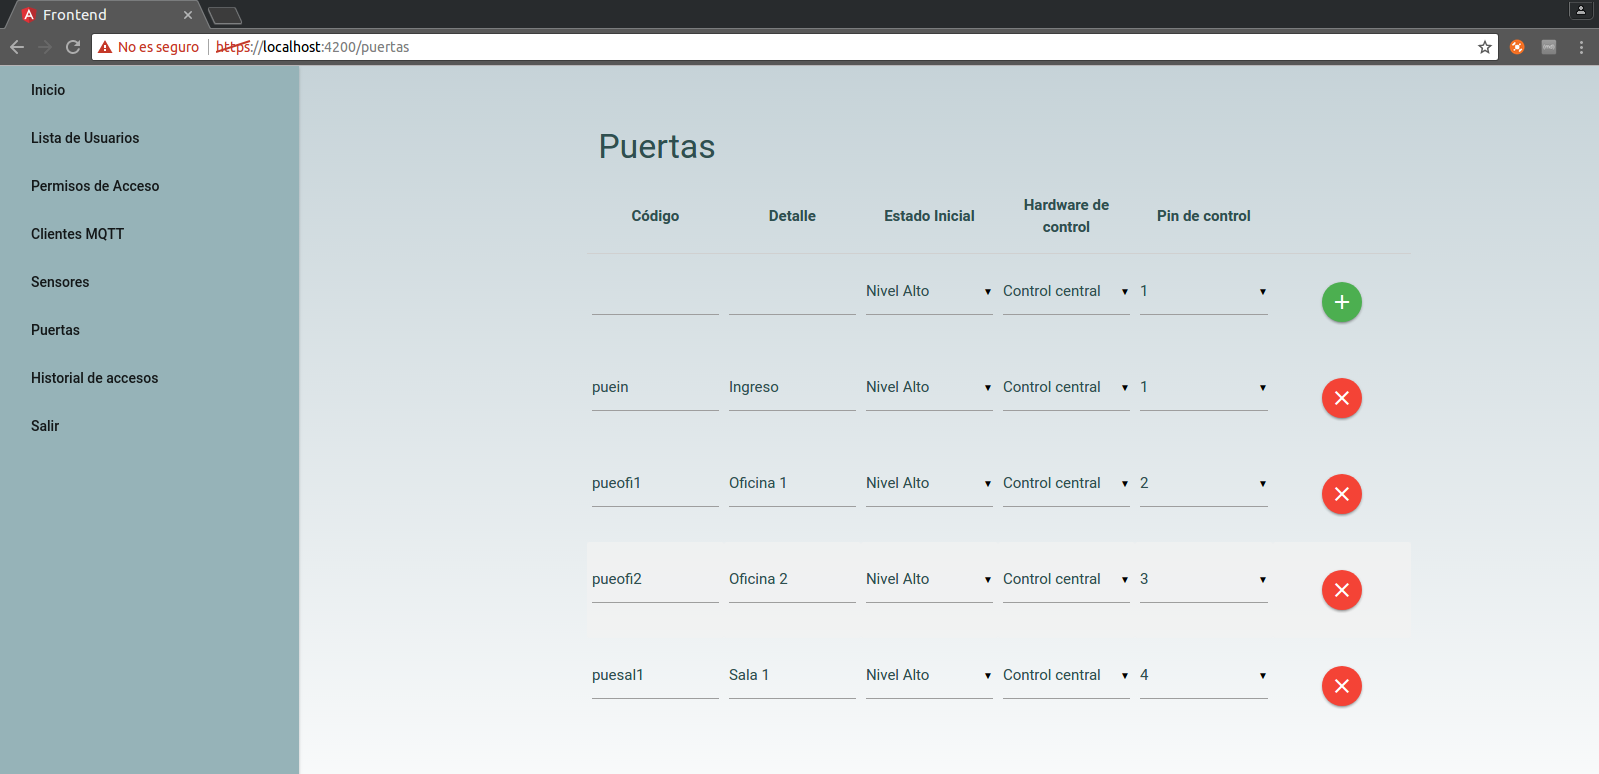
\includegraphics[width=0.95\textwidth]{ingenieria_proyecto/web_puertas.png}
    \caption*{\textbf{Fuente:} Elaboración propia}
    \label{fig:web_puertas}
  \end{figure}

  La página de historial de accesos contiene dos vistas, la primera muestra todos los accesos del día, pero tiene un campo de búsqueda donde se pueden revisar todos los accesos entre un rango de fechas.

  \begin{figure}[H]
    \centering
    \caption{Página de historial de accesos del servicio web}
    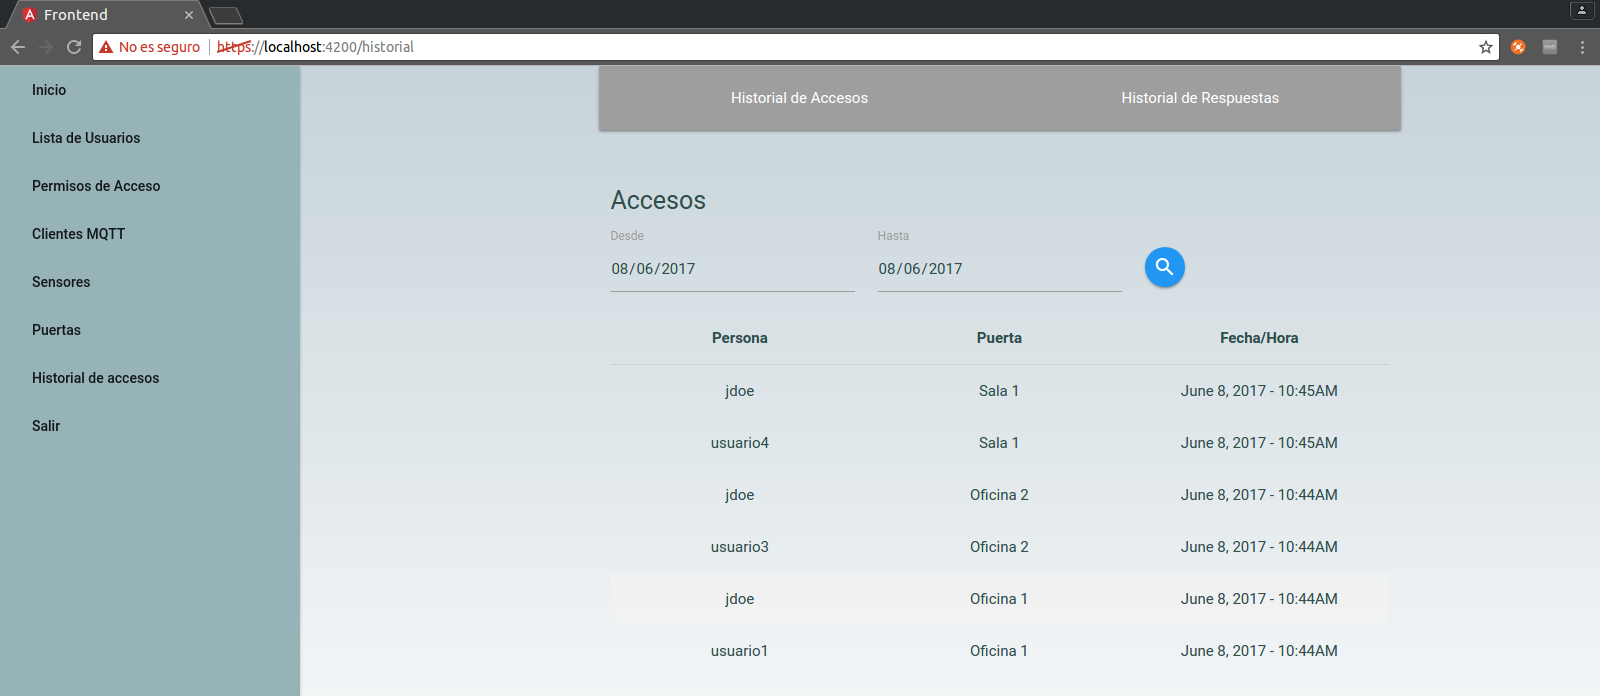
\includegraphics[width=0.95\textwidth]{ingenieria_proyecto/web_historial_accesos.png}
    \caption*{\textbf{Fuente:} Elaboración propia}
    \label{fig:web_historial_accesos}
  \end{figure}

  La vista de historial de respuestas alberga todos los comandos enviados hacia los sensores y las respuestas recibidas de los mismos de manera legible de acuerdo a los valores indicados en el manual del sensor ZFM-20 \cite{manual:fingerprint_ZFM-20}.

  \begin{figure}[H]
    \centering
    \caption{Página de historial de respuestas del servicio web}
    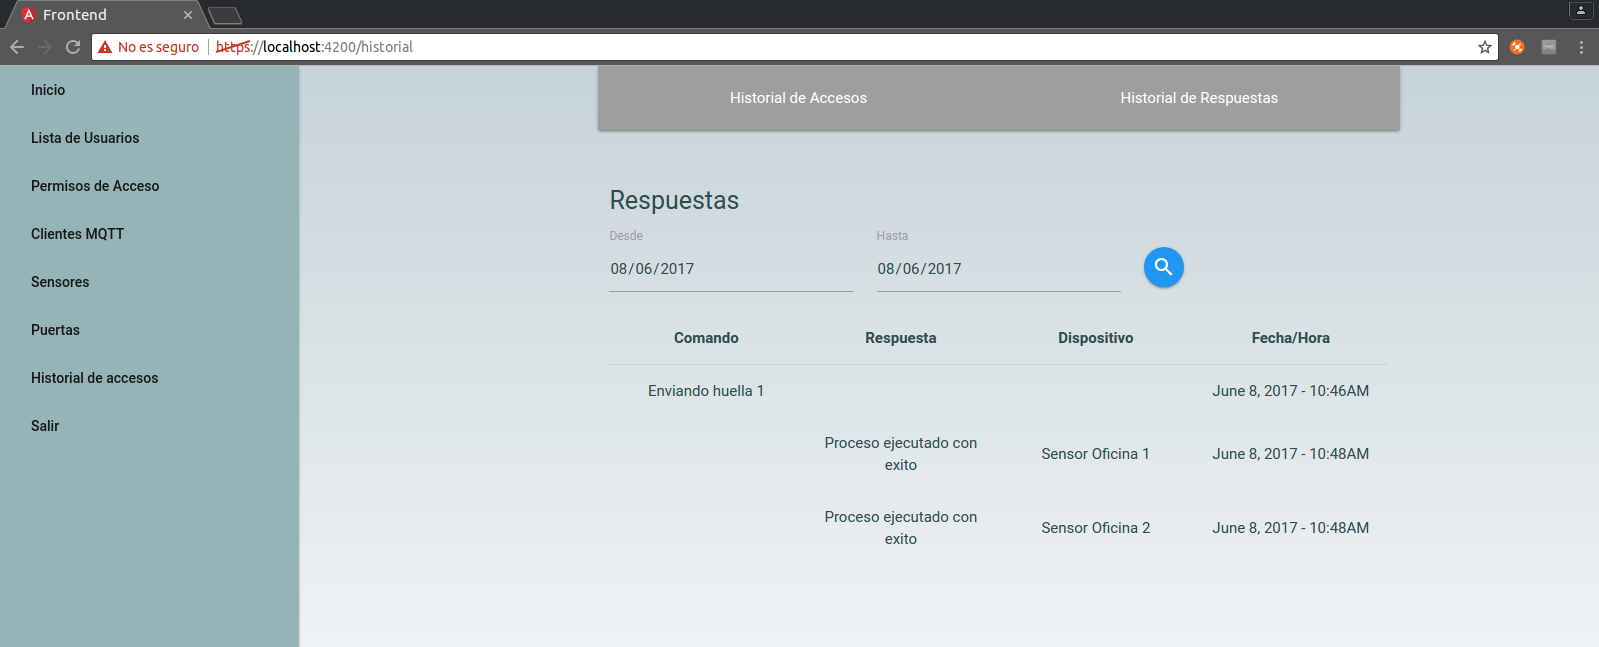
\includegraphics[width=0.95\textwidth]{ingenieria_proyecto/web_historial_respuestas.png}
    \caption*{\textbf{Fuente:} Elaboración propia}
    \label{fig:web_historial_respuestas}
  \end{figure}

  Cuando un usuario registrado en el servidor LDAP ingresa con su contraseña, puede acceder a una página donde solo se muestran las puertas por las que tiene acceso, para que dicho usuario pueda abrir las puertas desde este mismo sistema web. Esto es muy útil en caso de que el sistema se instale por ejemplo en una oficina con una persona en recepción, para que esta persona desde su computadora pueda abrir las puertas a los visitantes o a las personas que no tengan registrada su huella y no tenga que colocar su dedo en sensor cada vez que deba abrir una puerta.

  \begin{figure}[H]
    \centering
    \caption{Página de usuario sin privilegios del servicio web}
    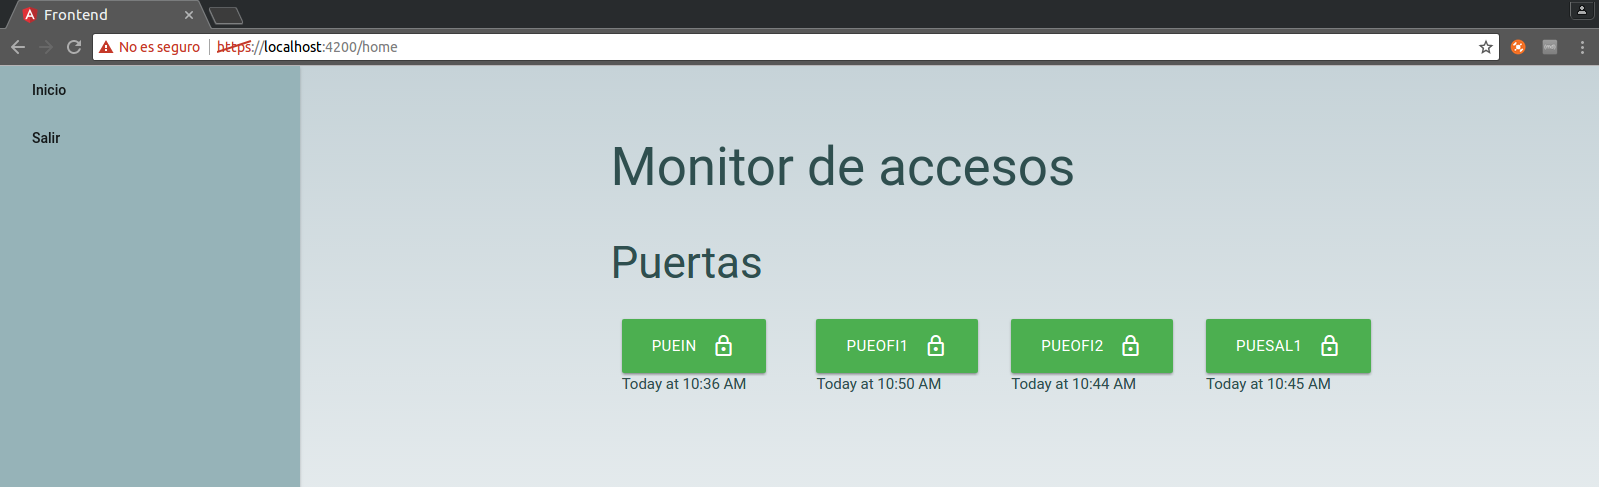
\includegraphics[width=0.95\textwidth]{ingenieria_proyecto/web_usuario_normal.png}
    \caption*{\textbf{Fuente:} Elaboración propia}
    \label{fig:web_usuario_normal}
  \end{figure}

  Por último tanto para el usuario administrador como para el usuario sin privilegios, se tiene la opción \textbf{Salir}, que como indica cierra la sesión abierta del navegador y regresa a la pantalla de login. Por defecto las sesiones solo pueden durar abiertas 4 horas, después de ese tiempo la aplicación cerrará la sesión automáticamente y volverá a la pantalla de login, donde el usuario tendrá que introducir sus credenciales nuevamente. Esto es una medida de seguridad en caso de que la persona de recepción haya terminado su turno laboral y se retire dejando su computadora encendida y que otra persona intente abrir una puerta con la misma cuenta abierta de la persona que cometió el descuido.

  \bibliografia

\end{document}
